\documentclass[10pt,a4paper,oneside]{article}

% ---------------------------------------------------------------------------
% Preâmbulo base do repositório: fonte, mancha, pacotes, legenda, título e
% cabeçalho. Compile de dentro de `docs/product/`.
% ---------------------------------------------------------------------------
\usepackage[brazil]{babel}
% =====================================================================
%  Preâmbulo base: pacotes, tipografia e convenções de todo documento
%  LaTeX do repositório
%
%  Origem: `config/preambulo.tex` do documento de projeto do rhae-sensor.
%  As seções abaixo seguem a ordem de lá, e o que difere está marcado
%  com DIFERENÇA.
%
%  Convenções tipográficas e de apresentação adotadas
%    ISO 216        formato A4
%    ISO 80000-1    números e unidades (vírgula decimal, espaço fino entre
%                   grupos de três algarismos, unidade em tipo romano)
%    Tabelas sem filetes verticais (booktabs); legenda de tabela acima,
%    de figura abaixo.
%
%  Uso, antes do `\begin{document}`:
%    report/*.tex          via `\usepackage{estilo-reporte}`, que carrega este
%    docs/product/*.tex    % =====================================================================
%  Preâmbulo base: pacotes, tipografia e convenções de todo documento
%  LaTeX do repositório
%
%  Origem: `config/preambulo.tex` do documento de projeto do rhae-sensor.
%  As seções abaixo seguem a ordem de lá, e o que difere está marcado
%  com DIFERENÇA.
%
%  Convenções tipográficas e de apresentação adotadas
%    ISO 216        formato A4
%    ISO 80000-1    números e unidades (vírgula decimal, espaço fino entre
%                   grupos de três algarismos, unidade em tipo romano)
%    Tabelas sem filetes verticais (booktabs); legenda de tabela acima,
%    de figura abaixo.
%
%  Uso, antes do `\begin{document}`:
%    report/*.tex          via `\usepackage{estilo-reporte}`, que carrega este
%    docs/product/*.tex    % =====================================================================
%  Preâmbulo base: pacotes, tipografia e convenções de todo documento
%  LaTeX do repositório
%
%  Origem: `config/preambulo.tex` do documento de projeto do rhae-sensor.
%  As seções abaixo seguem a ordem de lá, e o que difere está marcado
%  com DIFERENÇA.
%
%  Convenções tipográficas e de apresentação adotadas
%    ISO 216        formato A4
%    ISO 80000-1    números e unidades (vírgula decimal, espaço fino entre
%                   grupos de três algarismos, unidade em tipo romano)
%    Tabelas sem filetes verticais (booktabs); legenda de tabela acima,
%    de figura abaixo.
%
%  Uso, antes do `\begin{document}`:
%    report/*.tex          via `\usepackage{estilo-reporte}`, que carrega este
%    docs/product/*.tex    \input{../../report/config/preambulo}
%
%  FORMA DE MANUAL TÉCNICO. Fonte, números, legendas e pacotes vêm da
%  origem. A forma da página não: é de manual de referência, e não de
%  artigo. Coluna única, títulos recuados para a esquerda do texto,
%  rodapé com identificação e "página X de Y" em toda página, avisos com
%  palavra de sinal (ANSI Z535.6), passos numerados e histórico de
%  revisões (IEC/IEEE 82079-1). O desenho de página segue a classe
%  `refman` do CTAN.
%
%  O documento carrega `babel` ANTES deste arquivo. Documento deitado, que
%  existe para caber tabela larga, carrega também `geometry` antes; aí a
%  margem de manual não entra e os títulos não avançam.
%
%  Motor: pdflatex. Charis SIL, newtxmath e Bera Mono entram como Type 1
%  em T1, e a matemática do newtxmath não passa pelo `unicode-math`.
% =====================================================================
\RequirePackage{iftex}
\RequirePDFTeX
% Este arquivo entra tanto de um `.tex` quanto de dentro do
% `estilo-reporte.sty`, onde o `@` ja e letra. O codigo de categoria e
% devolvido como estava, e nao forcado a "outro" no fim.
\edef\pbrestauraarroba{\catcode`\noexpand\@=\the\catcode`\@\relax}
\makeatletter

% ---------------------------------------------------------------------
%  Fontes, idioma e microtipografia
% ---------------------------------------------------------------------
\usepackage[T1]{fontenc}
\usepackage[utf8]{inputenc}
% DIFERENÇA: o idioma é do documento, porque há documento em inglês.
\@ifpackageloaded{babel}{}{\usepackage[brazilian]{babel}}
\usepackage{CharisSIL}
\usepackage[charter]{newtxmath}
\usepackage[scaled=0.83]{beramono}
\usepackage[protrusion=true,expansion=true,tracking=true]{microtype}
\SetTracking{encoding=*,shape=sc}{40}
% DIFERENÇA: a origem não usa sem serifa. Os documentos daqui pedem
% `\sffamily` em título, tabela e nota; sem esta linha ela cairia na
% Computer Modern Sans, que não pertence ao conjunto. Uma família só.
\renewcommand{\sfdefault}{\rmdefault}

% DIFERENÇA: mancha de manual, e não a coluna de 468 pt da origem. A4 com
% 22 mm de margem de cada lado, 166 mm úteis. O texto corre em 152 mm e
% os 14 mm da esquerda são o recuo dos títulos: o bastante para o título
% sair do alinhamento do texto, sem deixar coluna vazia ao lado dele. A
% primeira versão reservava 40 mm, e a margem ficava em branco em toda
% página que não fosse título; o documento crescia um terço só por isso.
% `\margemmanual` é quanto os títulos, o cabeçalho e o rodapé avançam
% para a esquerda; vale zero quando o documento traz mancha própria.
% A altura é de 253 mm, a mesma da mancha anterior, porque as tabelas
% deitadas foram dimensionadas para ela.
\newlength{\margemmanual}
\@ifpackageloaded{geometry}{\setlength{\margemmanual}{0pt}}{%
  \setlength{\margemmanual}{14mm}%
  \usepackage[a4paper,left=36mm,right=22mm,top=20mm,bottom=24mm,
              headheight=14pt,headsep=7mm,footskip=12mm]{geometry}}

\usepackage{amsmath}
\usepackage[dvipsnames,table]{xcolor}
\usepackage{graphicx}
\usepackage{tikz}
\usepackage{booktabs}
\usepackage{tabularx}
\usepackage{array}
\usepackage{xltabular}
\usepackage{float}
\usepackage{pdflscape}
\usepackage{rotating}
% Página com o conteúdo girado, mas exibida em retrato no leitor de PDF
\newenvironment{paisagemretrato}{\begingroup\def\PLS@AddRotate##1{}\landscape}{\endlandscape\endgroup}
\usepackage{enumitem}
\usepackage{changepage}
\usepackage[most]{tcolorbox}
\usepackage{caption}
\usepackage{titlesec}
\usepackage{fancyhdr}
\usepackage{lastpage}
\usepackage{csquotes}
\usepackage{siunitx}
% DIFERENÇA: sem `biblatex`. Nenhum documento daqui tem `.bib`; as
% referências são listas escritas à mão.
\usepackage{xurl}
\usepackage[hidelinks,pdfusetitle]{hyperref}

% ---------------------------------------------------------------------
%  Números e unidades (ISO 80000-1)
% ---------------------------------------------------------------------
\sisetup{
  output-decimal-marker = {,},
  group-separator       = {\,},
  group-minimum-digits  = 4,
  exponent-product      = \cdot,
  uncertainty-mode      = separate,
  range-phrase          = {\,a\,},
  list-pair-separator   = {\ e\ },
  list-final-separator  = {\ e\ },
  per-mode              = symbol,
}

% ---------------------------------------------------------------------
%  Parágrafo, listas e flutuantes
% ---------------------------------------------------------------------
% DIFERENÇA: parágrafo em bloco, separado por espaço e sem recuo, que é
% o de manual; a origem recua 1 em.
\setlength{\parindent}{0pt}
\setlength{\parskip}{0.45em plus 0.1em}
\linespread{1.04}
\setlist{itemsep=0.1em,topsep=0.3em,leftmargin=1.4em}
\renewcommand{\arraystretch}{1.15}
\setlength{\tabcolsep}{5pt}
\setlength{\LTpre}{0.8em}
\setlength{\LTpost}{0.4em}

% Legendas no padrão Elsevier: \enquote{Fig. 1.} seguido do texto, alinhado à esquerda;
% \enquote{Tabela 1} numa linha e o título na linha seguinte
\DeclareCaptionLabelSeparator{travessao}{\ — }
% `babel` guarda os nomes por idioma, e o nome da opção varia entre os
% documentos. Entra em cada um que estiver carregado.
\@for\pb@idioma:=brazilian,brazil,portuguese,portuges,american,english\do{%
  \@ifundefined{captions\pb@idioma}{}{%
    \expandafter\addto\csname captions\pb@idioma\endcsname{\renewcommand{\figurename}{Fig.}}}}
\captionsetup{font=footnotesize,labelfont=bf,justification=justified,
              singlelinecheck=false,skip=5pt}
\captionsetup[figure]{position=bottom,labelsep=period}
\captionsetup[table]{position=top,labelsep=newline}
% DIFERENÇA: a origem fixa todo flutuante onde aparece (`H`). Aqui ele
% tenta o lugar e, se não couber no resto da página, sobe para a seguinte
% e o texto continua: com `H`, a tabela que não cabia deixava o fim da
% página em branco.
\floatplacement{table}{!htbp}
\floatplacement{figure}{!htbp}
\renewcommand{\topfraction}{0.9}
\renewcommand{\bottomfraction}{0.8}
\renewcommand{\textfraction}{0.08}
\renewcommand{\floatpagefraction}{0.75}

\newcolumntype{Y}{>{\raggedright\arraybackslash}X}
\newcolumntype{L}[1]{>{\raggedright\arraybackslash}p{#1}}
\newcolumntype{C}[1]{>{\centering\arraybackslash}p{#1}}
\newcolumntype{R}[1]{>{\raggedleft\arraybackslash}p{#1}}

% ---------------------------------------------------------------------
%  Títulos de seção (ISO 2145)
% ---------------------------------------------------------------------
% DIFERENÇA: título de manual. Seção e subseção avançam 14 mm para a
% esquerda do texto e ocupam a largura útil; a seção leva um fio acima.
% Número sem ponto final, três níveis numerados. Os três níveis têm o
% corpo do texto ou pouco mais: o nível se lê pelo fio, pelo recuo e
% pelo itálico do terceiro, e não pelo tamanho.
\setcounter{secnumdepth}{3}
\titleformat{\section}[block]
  {\titlerule[0.8pt]\vspace{0.5ex}\normalfont\large\bfseries\raggedright}{\thesection}{0.8em}{}
\titleformat{\subsection}{\normalfont\normalsize\bfseries\raggedright}{\thesubsection}{0.8em}{}
\titleformat{\subsubsection}{\normalfont\normalsize\bfseries\itshape\raggedright}{\thesubsubsection}{0.8em}{}
\titlespacing*{\section}{-\margemmanual}{1.5em plus 0.4em minus 0.2em}{0.5em plus 0.1em}
\titlespacing*{\subsection}{-\margemmanual}{1.1em plus 0.3em minus 0.2em}{0.3em plus 0.1em}
\titlespacing*{\subsubsection}{0pt}{0.9em plus 0.2em minus 0.2em}{0.2em}

% ---------------------------------------------------------------------
%  Identificação, cabeçalho e rodapé
% ---------------------------------------------------------------------
% Todo campo é do documento, por `\renewcommand` depois deste arquivo.
% Sem isso: o código é o nome do arquivo, a data é a da compilação em
% ISO 8601, e versão e responsável ficam vazios e somem.
\providecommand{\doctitulo}{}
\providecommand{\docsubtitulo}{}
\providecommand{\doccodigo}{\jobname}
\providecommand{\docversao}{}
\providecommand{\docresponsavel}{}
\providecommand{\docdata}{\the\year-\two@digits\month-\two@digits\day}

% Cabeçalho: título à esquerda, seção corrente à direita. Rodapé: código,
% versão e data à esquerda, "página X de Y" à direita. Os dois ocupam a
% largura útil, margem de título incluída.
\newcommand{\pb@identificacao}{%
  \texttt{\doccodigo}%
  \ifx\docversao\@empty\else\enspace\textperiodcentered\enspace versão \docversao\fi
  \enspace\textperiodcentered\enspace\docdata}
\pagestyle{fancy}
\fancyhf{}
\fancyhfoffset[L]{\margemmanual}
\fancyhead[L]{\footnotesize\bfseries\doctitulo}
\fancyhead[R]{\footnotesize\itshape\nouppercase{\rightmark}}
\fancyfoot[L]{\footnotesize\pb@identificacao}
\fancyfoot[R]{\footnotesize\thepage\ de \pageref*{LastPage}}
\renewcommand{\headrulewidth}{0.4pt}
\renewcommand{\footrulewidth}{0.4pt}
\fancypagestyle{plain}{}
% Página de rosto: sem cabeçalho, porque o título já está nela.
\fancypagestyle{rosto}{\fancyhead{}\renewcommand{\headrulewidth}{0pt}}

% ---------------------------------------------------------------------
%  Marca
% ---------------------------------------------------------------------
% DIFERENÇA: a origem não tem marca. Aqui todo documento abre com o
% logotipo Solara, versão para fundo claro. O caminho depende de onde se
% compila: `report/` ou `docs/product/`.
\IfFileExists{../docs/img/solara-logo-on-light.png}%
  {\newcommand{\marcaarquivo}{../docs/img/solara-logo-on-light.png}}%
  {\newcommand{\marcaarquivo}{../img/solara-logo-on-light.png}}
% \marcadoc[largura]: o logotipo tem proporção 7:1, então 30 mm dão
% 4,3 mm de altura.
\newcommand{\marcadoc}[1][30mm]{\includegraphics[width=#1]{\marcaarquivo}}

% ---------------------------------------------------------------------
%  Rosto e histórico de revisões
% ---------------------------------------------------------------------
% \rosto: marca, título, subtítulo e a tabela de identificação. Lê os
% campos `\doc...`; linha de campo vazio não sai.
\newcommand{\pb@linha}[2]{\ifx#2\@empty\else #1 & #2 \\\fi}
\newcommand{\rosto}{%
  \thispagestyle{rosto}%
  \begin{adjustwidth}{-\margemmanual}{0pt}
    \raggedright
    \marcadoc[45mm]\par\vspace{16mm}
    {\fontsize{24}{29}\selectfont\bfseries\doctitulo\par}
    \ifx\docsubtitulo\@empty\else
      \vspace{3mm}{\Large\color{cinza}\docsubtitulo\par}\fi
    \vspace{9mm}{\hrule height 0.8pt}\vspace{4mm}
    {\small\renewcommand{\arraystretch}{1.25}%
     \begin{tabular}{@{}>{\bfseries}p{28mm}p{110mm}@{}}
       Documento & \texttt{\doccodigo} \\
       \pb@linha{Versão}{\docversao}%
       Data & \docdata \\
       \pb@linha{Responsável}{\docresponsavel}%
     \end{tabular}\par}
  \end{adjustwidth}
  \vspace{10mm}}

% Histórico de revisões: uma linha por versão, a mais recente em cima.
%   \begin{historico}
%     0.2 & 2026-10-03 & O que mudou \\
%   \end{historico}
\newenvironment{historico}
  {\par\medskip\noindent\small
   \begin{tabular}{@{}p{16mm}p{24mm}p{\dimexpr\linewidth-40mm-4\tabcolsep\relax}@{}}
   \toprule \textbf{Versão} & \textbf{Data} & \textbf{Alteração} \\ \midrule}
  {\bottomrule\end{tabular}\par\medskip}

% ---------------------------------------------------------------------
%  Avisos (ANSI Z535.6) e nota
% ---------------------------------------------------------------------
% Quatro palavras de sinal, em hierarquia fixa. As três primeiras são de
% dano a pessoa; AVISO é de dano a equipamento ou a dado. Cada mensagem
% diz o risco, como evitar e a consequência. NOTA não é aviso: é
% informação de apoio.
\definecolor{sinalperigo}{HTML}{C8102E}
\definecolor{sinalatencao}{HTML}{E87722}
\definecolor{sinalcuidado}{HTML}{F2C200}
\definecolor{sinalaviso}{HTML}{00539B}
\definecolor{sinalnota}{HTML}{5F5F5F}
% #1 palavra, #2 cor da faixa, #3 cor da letra sobre a faixa
\newtcolorbox{pb@mensagem}[3]{enhanced,breakable,sharp corners,
  boxrule=0pt,frame hidden,borderline west={3pt}{0pt}{#2},
  colback=#2!7,left=9pt,right=7pt,top=5pt,bottom=5pt,
  before skip=0.9em,after skip=0.9em,fontupper=\small,
  before upper={\colorbox{#2}{\textcolor{#3}{\footnotesize\bfseries #1}}\enspace}}
\newenvironment{perigo}{\csname pb@mensagem\endcsname{PERIGO}{sinalperigo}{white}}{\csname endpb@mensagem\endcsname}
\newenvironment{atencao}{\csname pb@mensagem\endcsname{ATENÇÃO}{sinalatencao}{black}}{\csname endpb@mensagem\endcsname}
\newenvironment{cuidado}{\csname pb@mensagem\endcsname{CUIDADO}{sinalcuidado}{black}}{\csname endpb@mensagem\endcsname}
\newenvironment{aviso}{\csname pb@mensagem\endcsname{AVISO}{sinalaviso}{white}}{\csname endpb@mensagem\endcsname}
\newenvironment{nota}{\csname pb@mensagem\endcsname{NOTA}{sinalnota}{white}}{\csname endpb@mensagem\endcsname}

% ---------------------------------------------------------------------
%  Procedimento
% ---------------------------------------------------------------------
% Passos numerados, uma ação por passo, no imperativo. A pré-condição vem
% antes da lista e o resultado esperado depois.
\newlist{passos}{enumerate}{2}
\setlist[passos,1]{label=\textbf{\arabic*.},leftmargin=2.2em,itemsep=0.45em,topsep=0.6em}
\setlist[passos,2]{label=\alph*),leftmargin=1.8em,itemsep=0.2em,topsep=0.2em}
\newcommand{\precondicao}[1]{\par\smallskip\noindent\textbf{Antes de começar.}\enspace#1\par}
\newcommand{\resultado}[1]{\par\smallskip\noindent\textbf{Resultado.}\enspace#1\par}

% Bloco na largura útil inteira, margem de título incluída: para tabela
% ou figura que não cabe nos 152 mm do texto.
\newenvironment{larga}{\begin{adjustwidth}{-\margemmanual}{0pt}}{\end{adjustwidth}}
% O mesmo dentro de `table` ou `figure`, onde `adjustwidth` não alcança:
% uma caixa na largura útil, puxada para a margem. Não quebra página.
% Dentro dela a largura é `\linewidth`, e não `\textwidth`.
\newenvironment{tabelalarga}
  {\noindent\hspace*{-\margemmanual}%
   \begin{minipage}{\dimexpr\linewidth+\margemmanual\relax}\centering}
  {\end{minipage}}

% ---------------------------------------------------------------------
%  Campos e figuras
% ---------------------------------------------------------------------
\definecolor{cinza}{gray}{0.40}

% \figuradoc[largura]{caminho}; sem o arquivo, uma caixa marca a pendência
\newcommand{\figuradoc}[2][\linewidth]{%
  \IfFileExists{#2}%
    {\includegraphics[width=#1,height=0.80\textheight,keepaspectratio]{#2}}%
    {\fbox{\parbox[c][45mm][c]{\dimexpr#1-2\fboxsep-2\fboxrule\relax}%
      {\centering\small\color{cinza}\itshape[figura em preparação]}}}}

\pbrestauraarroba

%
%  FORMA DE MANUAL TÉCNICO. Fonte, números, legendas e pacotes vêm da
%  origem. A forma da página não: é de manual de referência, e não de
%  artigo. Coluna única, títulos recuados para a esquerda do texto,
%  rodapé com identificação e "página X de Y" em toda página, avisos com
%  palavra de sinal (ANSI Z535.6), passos numerados e histórico de
%  revisões (IEC/IEEE 82079-1). O desenho de página segue a classe
%  `refman` do CTAN.
%
%  O documento carrega `babel` ANTES deste arquivo. Documento deitado, que
%  existe para caber tabela larga, carrega também `geometry` antes; aí a
%  margem de manual não entra e os títulos não avançam.
%
%  Motor: pdflatex. Charis SIL, newtxmath e Bera Mono entram como Type 1
%  em T1, e a matemática do newtxmath não passa pelo `unicode-math`.
% =====================================================================
\RequirePackage{iftex}
\RequirePDFTeX
% Este arquivo entra tanto de um `.tex` quanto de dentro do
% `estilo-reporte.sty`, onde o `@` ja e letra. O codigo de categoria e
% devolvido como estava, e nao forcado a "outro" no fim.
\edef\pbrestauraarroba{\catcode`\noexpand\@=\the\catcode`\@\relax}
\makeatletter

% ---------------------------------------------------------------------
%  Fontes, idioma e microtipografia
% ---------------------------------------------------------------------
\usepackage[T1]{fontenc}
\usepackage[utf8]{inputenc}
% DIFERENÇA: o idioma é do documento, porque há documento em inglês.
\@ifpackageloaded{babel}{}{\usepackage[brazilian]{babel}}
\usepackage{CharisSIL}
\usepackage[charter]{newtxmath}
\usepackage[scaled=0.83]{beramono}
\usepackage[protrusion=true,expansion=true,tracking=true]{microtype}
\SetTracking{encoding=*,shape=sc}{40}
% DIFERENÇA: a origem não usa sem serifa. Os documentos daqui pedem
% `\sffamily` em título, tabela e nota; sem esta linha ela cairia na
% Computer Modern Sans, que não pertence ao conjunto. Uma família só.
\renewcommand{\sfdefault}{\rmdefault}

% DIFERENÇA: mancha de manual, e não a coluna de 468 pt da origem. A4 com
% 22 mm de margem de cada lado, 166 mm úteis. O texto corre em 152 mm e
% os 14 mm da esquerda são o recuo dos títulos: o bastante para o título
% sair do alinhamento do texto, sem deixar coluna vazia ao lado dele. A
% primeira versão reservava 40 mm, e a margem ficava em branco em toda
% página que não fosse título; o documento crescia um terço só por isso.
% `\margemmanual` é quanto os títulos, o cabeçalho e o rodapé avançam
% para a esquerda; vale zero quando o documento traz mancha própria.
% A altura é de 253 mm, a mesma da mancha anterior, porque as tabelas
% deitadas foram dimensionadas para ela.
\newlength{\margemmanual}
\@ifpackageloaded{geometry}{\setlength{\margemmanual}{0pt}}{%
  \setlength{\margemmanual}{14mm}%
  \usepackage[a4paper,left=36mm,right=22mm,top=20mm,bottom=24mm,
              headheight=14pt,headsep=7mm,footskip=12mm]{geometry}}

\usepackage{amsmath}
\usepackage[dvipsnames,table]{xcolor}
\usepackage{graphicx}
\usepackage{tikz}
\usepackage{booktabs}
\usepackage{tabularx}
\usepackage{array}
\usepackage{xltabular}
\usepackage{float}
\usepackage{pdflscape}
\usepackage{rotating}
% Página com o conteúdo girado, mas exibida em retrato no leitor de PDF
\newenvironment{paisagemretrato}{\begingroup\def\PLS@AddRotate##1{}\landscape}{\endlandscape\endgroup}
\usepackage{enumitem}
\usepackage{changepage}
\usepackage[most]{tcolorbox}
\usepackage{caption}
\usepackage{titlesec}
\usepackage{fancyhdr}
\usepackage{lastpage}
\usepackage{csquotes}
\usepackage{siunitx}
% DIFERENÇA: sem `biblatex`. Nenhum documento daqui tem `.bib`; as
% referências são listas escritas à mão.
\usepackage{xurl}
\usepackage[hidelinks,pdfusetitle]{hyperref}

% ---------------------------------------------------------------------
%  Números e unidades (ISO 80000-1)
% ---------------------------------------------------------------------
\sisetup{
  output-decimal-marker = {,},
  group-separator       = {\,},
  group-minimum-digits  = 4,
  exponent-product      = \cdot,
  uncertainty-mode      = separate,
  range-phrase          = {\,a\,},
  list-pair-separator   = {\ e\ },
  list-final-separator  = {\ e\ },
  per-mode              = symbol,
}

% ---------------------------------------------------------------------
%  Parágrafo, listas e flutuantes
% ---------------------------------------------------------------------
% DIFERENÇA: parágrafo em bloco, separado por espaço e sem recuo, que é
% o de manual; a origem recua 1 em.
\setlength{\parindent}{0pt}
\setlength{\parskip}{0.45em plus 0.1em}
\linespread{1.04}
\setlist{itemsep=0.1em,topsep=0.3em,leftmargin=1.4em}
\renewcommand{\arraystretch}{1.15}
\setlength{\tabcolsep}{5pt}
\setlength{\LTpre}{0.8em}
\setlength{\LTpost}{0.4em}

% Legendas no padrão Elsevier: \enquote{Fig. 1.} seguido do texto, alinhado à esquerda;
% \enquote{Tabela 1} numa linha e o título na linha seguinte
\DeclareCaptionLabelSeparator{travessao}{\ — }
% `babel` guarda os nomes por idioma, e o nome da opção varia entre os
% documentos. Entra em cada um que estiver carregado.
\@for\pb@idioma:=brazilian,brazil,portuguese,portuges,american,english\do{%
  \@ifundefined{captions\pb@idioma}{}{%
    \expandafter\addto\csname captions\pb@idioma\endcsname{\renewcommand{\figurename}{Fig.}}}}
\captionsetup{font=footnotesize,labelfont=bf,justification=justified,
              singlelinecheck=false,skip=5pt}
\captionsetup[figure]{position=bottom,labelsep=period}
\captionsetup[table]{position=top,labelsep=newline}
% DIFERENÇA: a origem fixa todo flutuante onde aparece (`H`). Aqui ele
% tenta o lugar e, se não couber no resto da página, sobe para a seguinte
% e o texto continua: com `H`, a tabela que não cabia deixava o fim da
% página em branco.
\floatplacement{table}{!htbp}
\floatplacement{figure}{!htbp}
\renewcommand{\topfraction}{0.9}
\renewcommand{\bottomfraction}{0.8}
\renewcommand{\textfraction}{0.08}
\renewcommand{\floatpagefraction}{0.75}

\newcolumntype{Y}{>{\raggedright\arraybackslash}X}
\newcolumntype{L}[1]{>{\raggedright\arraybackslash}p{#1}}
\newcolumntype{C}[1]{>{\centering\arraybackslash}p{#1}}
\newcolumntype{R}[1]{>{\raggedleft\arraybackslash}p{#1}}

% ---------------------------------------------------------------------
%  Títulos de seção (ISO 2145)
% ---------------------------------------------------------------------
% DIFERENÇA: título de manual. Seção e subseção avançam 14 mm para a
% esquerda do texto e ocupam a largura útil; a seção leva um fio acima.
% Número sem ponto final, três níveis numerados. Os três níveis têm o
% corpo do texto ou pouco mais: o nível se lê pelo fio, pelo recuo e
% pelo itálico do terceiro, e não pelo tamanho.
\setcounter{secnumdepth}{3}
\titleformat{\section}[block]
  {\titlerule[0.8pt]\vspace{0.5ex}\normalfont\large\bfseries\raggedright}{\thesection}{0.8em}{}
\titleformat{\subsection}{\normalfont\normalsize\bfseries\raggedright}{\thesubsection}{0.8em}{}
\titleformat{\subsubsection}{\normalfont\normalsize\bfseries\itshape\raggedright}{\thesubsubsection}{0.8em}{}
\titlespacing*{\section}{-\margemmanual}{1.5em plus 0.4em minus 0.2em}{0.5em plus 0.1em}
\titlespacing*{\subsection}{-\margemmanual}{1.1em plus 0.3em minus 0.2em}{0.3em plus 0.1em}
\titlespacing*{\subsubsection}{0pt}{0.9em plus 0.2em minus 0.2em}{0.2em}

% ---------------------------------------------------------------------
%  Identificação, cabeçalho e rodapé
% ---------------------------------------------------------------------
% Todo campo é do documento, por `\renewcommand` depois deste arquivo.
% Sem isso: o código é o nome do arquivo, a data é a da compilação em
% ISO 8601, e versão e responsável ficam vazios e somem.
\providecommand{\doctitulo}{}
\providecommand{\docsubtitulo}{}
\providecommand{\doccodigo}{\jobname}
\providecommand{\docversao}{}
\providecommand{\docresponsavel}{}
\providecommand{\docdata}{\the\year-\two@digits\month-\two@digits\day}

% Cabeçalho: título à esquerda, seção corrente à direita. Rodapé: código,
% versão e data à esquerda, "página X de Y" à direita. Os dois ocupam a
% largura útil, margem de título incluída.
\newcommand{\pb@identificacao}{%
  \texttt{\doccodigo}%
  \ifx\docversao\@empty\else\enspace\textperiodcentered\enspace versão \docversao\fi
  \enspace\textperiodcentered\enspace\docdata}
\pagestyle{fancy}
\fancyhf{}
\fancyhfoffset[L]{\margemmanual}
\fancyhead[L]{\footnotesize\bfseries\doctitulo}
\fancyhead[R]{\footnotesize\itshape\nouppercase{\rightmark}}
\fancyfoot[L]{\footnotesize\pb@identificacao}
\fancyfoot[R]{\footnotesize\thepage\ de \pageref*{LastPage}}
\renewcommand{\headrulewidth}{0.4pt}
\renewcommand{\footrulewidth}{0.4pt}
\fancypagestyle{plain}{}
% Página de rosto: sem cabeçalho, porque o título já está nela.
\fancypagestyle{rosto}{\fancyhead{}\renewcommand{\headrulewidth}{0pt}}

% ---------------------------------------------------------------------
%  Marca
% ---------------------------------------------------------------------
% DIFERENÇA: a origem não tem marca. Aqui todo documento abre com o
% logotipo Solara, versão para fundo claro. O caminho depende de onde se
% compila: `report/` ou `docs/product/`.
\IfFileExists{../docs/img/solara-logo-on-light.png}%
  {\newcommand{\marcaarquivo}{../docs/img/solara-logo-on-light.png}}%
  {\newcommand{\marcaarquivo}{../img/solara-logo-on-light.png}}
% \marcadoc[largura]: o logotipo tem proporção 7:1, então 30 mm dão
% 4,3 mm de altura.
\newcommand{\marcadoc}[1][30mm]{\includegraphics[width=#1]{\marcaarquivo}}

% ---------------------------------------------------------------------
%  Rosto e histórico de revisões
% ---------------------------------------------------------------------
% \rosto: marca, título, subtítulo e a tabela de identificação. Lê os
% campos `\doc...`; linha de campo vazio não sai.
\newcommand{\pb@linha}[2]{\ifx#2\@empty\else #1 & #2 \\\fi}
\newcommand{\rosto}{%
  \thispagestyle{rosto}%
  \begin{adjustwidth}{-\margemmanual}{0pt}
    \raggedright
    \marcadoc[45mm]\par\vspace{16mm}
    {\fontsize{24}{29}\selectfont\bfseries\doctitulo\par}
    \ifx\docsubtitulo\@empty\else
      \vspace{3mm}{\Large\color{cinza}\docsubtitulo\par}\fi
    \vspace{9mm}{\hrule height 0.8pt}\vspace{4mm}
    {\small\renewcommand{\arraystretch}{1.25}%
     \begin{tabular}{@{}>{\bfseries}p{28mm}p{110mm}@{}}
       Documento & \texttt{\doccodigo} \\
       \pb@linha{Versão}{\docversao}%
       Data & \docdata \\
       \pb@linha{Responsável}{\docresponsavel}%
     \end{tabular}\par}
  \end{adjustwidth}
  \vspace{10mm}}

% Histórico de revisões: uma linha por versão, a mais recente em cima.
%   \begin{historico}
%     0.2 & 2026-10-03 & O que mudou \\
%   \end{historico}
\newenvironment{historico}
  {\par\medskip\noindent\small
   \begin{tabular}{@{}p{16mm}p{24mm}p{\dimexpr\linewidth-40mm-4\tabcolsep\relax}@{}}
   \toprule \textbf{Versão} & \textbf{Data} & \textbf{Alteração} \\ \midrule}
  {\bottomrule\end{tabular}\par\medskip}

% ---------------------------------------------------------------------
%  Avisos (ANSI Z535.6) e nota
% ---------------------------------------------------------------------
% Quatro palavras de sinal, em hierarquia fixa. As três primeiras são de
% dano a pessoa; AVISO é de dano a equipamento ou a dado. Cada mensagem
% diz o risco, como evitar e a consequência. NOTA não é aviso: é
% informação de apoio.
\definecolor{sinalperigo}{HTML}{C8102E}
\definecolor{sinalatencao}{HTML}{E87722}
\definecolor{sinalcuidado}{HTML}{F2C200}
\definecolor{sinalaviso}{HTML}{00539B}
\definecolor{sinalnota}{HTML}{5F5F5F}
% #1 palavra, #2 cor da faixa, #3 cor da letra sobre a faixa
\newtcolorbox{pb@mensagem}[3]{enhanced,breakable,sharp corners,
  boxrule=0pt,frame hidden,borderline west={3pt}{0pt}{#2},
  colback=#2!7,left=9pt,right=7pt,top=5pt,bottom=5pt,
  before skip=0.9em,after skip=0.9em,fontupper=\small,
  before upper={\colorbox{#2}{\textcolor{#3}{\footnotesize\bfseries #1}}\enspace}}
\newenvironment{perigo}{\csname pb@mensagem\endcsname{PERIGO}{sinalperigo}{white}}{\csname endpb@mensagem\endcsname}
\newenvironment{atencao}{\csname pb@mensagem\endcsname{ATENÇÃO}{sinalatencao}{black}}{\csname endpb@mensagem\endcsname}
\newenvironment{cuidado}{\csname pb@mensagem\endcsname{CUIDADO}{sinalcuidado}{black}}{\csname endpb@mensagem\endcsname}
\newenvironment{aviso}{\csname pb@mensagem\endcsname{AVISO}{sinalaviso}{white}}{\csname endpb@mensagem\endcsname}
\newenvironment{nota}{\csname pb@mensagem\endcsname{NOTA}{sinalnota}{white}}{\csname endpb@mensagem\endcsname}

% ---------------------------------------------------------------------
%  Procedimento
% ---------------------------------------------------------------------
% Passos numerados, uma ação por passo, no imperativo. A pré-condição vem
% antes da lista e o resultado esperado depois.
\newlist{passos}{enumerate}{2}
\setlist[passos,1]{label=\textbf{\arabic*.},leftmargin=2.2em,itemsep=0.45em,topsep=0.6em}
\setlist[passos,2]{label=\alph*),leftmargin=1.8em,itemsep=0.2em,topsep=0.2em}
\newcommand{\precondicao}[1]{\par\smallskip\noindent\textbf{Antes de começar.}\enspace#1\par}
\newcommand{\resultado}[1]{\par\smallskip\noindent\textbf{Resultado.}\enspace#1\par}

% Bloco na largura útil inteira, margem de título incluída: para tabela
% ou figura que não cabe nos 152 mm do texto.
\newenvironment{larga}{\begin{adjustwidth}{-\margemmanual}{0pt}}{\end{adjustwidth}}
% O mesmo dentro de `table` ou `figure`, onde `adjustwidth` não alcança:
% uma caixa na largura útil, puxada para a margem. Não quebra página.
% Dentro dela a largura é `\linewidth`, e não `\textwidth`.
\newenvironment{tabelalarga}
  {\noindent\hspace*{-\margemmanual}%
   \begin{minipage}{\dimexpr\linewidth+\margemmanual\relax}\centering}
  {\end{minipage}}

% ---------------------------------------------------------------------
%  Campos e figuras
% ---------------------------------------------------------------------
\definecolor{cinza}{gray}{0.40}

% \figuradoc[largura]{caminho}; sem o arquivo, uma caixa marca a pendência
\newcommand{\figuradoc}[2][\linewidth]{%
  \IfFileExists{#2}%
    {\includegraphics[width=#1,height=0.80\textheight,keepaspectratio]{#2}}%
    {\fbox{\parbox[c][45mm][c]{\dimexpr#1-2\fboxsep-2\fboxrule\relax}%
      {\centering\small\color{cinza}\itshape[figura em preparação]}}}}

\pbrestauraarroba

%
%  FORMA DE MANUAL TÉCNICO. Fonte, números, legendas e pacotes vêm da
%  origem. A forma da página não: é de manual de referência, e não de
%  artigo. Coluna única, títulos recuados para a esquerda do texto,
%  rodapé com identificação e "página X de Y" em toda página, avisos com
%  palavra de sinal (ANSI Z535.6), passos numerados e histórico de
%  revisões (IEC/IEEE 82079-1). O desenho de página segue a classe
%  `refman` do CTAN.
%
%  O documento carrega `babel` ANTES deste arquivo. Documento deitado, que
%  existe para caber tabela larga, carrega também `geometry` antes; aí a
%  margem de manual não entra e os títulos não avançam.
%
%  Motor: pdflatex. Charis SIL, newtxmath e Bera Mono entram como Type 1
%  em T1, e a matemática do newtxmath não passa pelo `unicode-math`.
% =====================================================================
\RequirePackage{iftex}
\RequirePDFTeX
% Este arquivo entra tanto de um `.tex` quanto de dentro do
% `estilo-reporte.sty`, onde o `@` ja e letra. O codigo de categoria e
% devolvido como estava, e nao forcado a "outro" no fim.
\edef\pbrestauraarroba{\catcode`\noexpand\@=\the\catcode`\@\relax}
\makeatletter

% ---------------------------------------------------------------------
%  Fontes, idioma e microtipografia
% ---------------------------------------------------------------------
\usepackage[T1]{fontenc}
\usepackage[utf8]{inputenc}
% DIFERENÇA: o idioma é do documento, porque há documento em inglês.
\@ifpackageloaded{babel}{}{\usepackage[brazilian]{babel}}
\usepackage{CharisSIL}
\usepackage[charter]{newtxmath}
\usepackage[scaled=0.83]{beramono}
\usepackage[protrusion=true,expansion=true,tracking=true]{microtype}
\SetTracking{encoding=*,shape=sc}{40}
% DIFERENÇA: a origem não usa sem serifa. Os documentos daqui pedem
% `\sffamily` em título, tabela e nota; sem esta linha ela cairia na
% Computer Modern Sans, que não pertence ao conjunto. Uma família só.
\renewcommand{\sfdefault}{\rmdefault}

% DIFERENÇA: mancha de manual, e não a coluna de 468 pt da origem. A4 com
% 22 mm de margem de cada lado, 166 mm úteis. O texto corre em 152 mm e
% os 14 mm da esquerda são o recuo dos títulos: o bastante para o título
% sair do alinhamento do texto, sem deixar coluna vazia ao lado dele. A
% primeira versão reservava 40 mm, e a margem ficava em branco em toda
% página que não fosse título; o documento crescia um terço só por isso.
% `\margemmanual` é quanto os títulos, o cabeçalho e o rodapé avançam
% para a esquerda; vale zero quando o documento traz mancha própria.
% A altura é de 253 mm, a mesma da mancha anterior, porque as tabelas
% deitadas foram dimensionadas para ela.
\newlength{\margemmanual}
\@ifpackageloaded{geometry}{\setlength{\margemmanual}{0pt}}{%
  \setlength{\margemmanual}{14mm}%
  \usepackage[a4paper,left=36mm,right=22mm,top=20mm,bottom=24mm,
              headheight=14pt,headsep=7mm,footskip=12mm]{geometry}}

\usepackage{amsmath}
\usepackage[dvipsnames,table]{xcolor}
\usepackage{graphicx}
\usepackage{tikz}
\usepackage{booktabs}
\usepackage{tabularx}
\usepackage{array}
\usepackage{xltabular}
\usepackage{float}
\usepackage{pdflscape}
\usepackage{rotating}
% Página com o conteúdo girado, mas exibida em retrato no leitor de PDF
\newenvironment{paisagemretrato}{\begingroup\def\PLS@AddRotate##1{}\landscape}{\endlandscape\endgroup}
\usepackage{enumitem}
\usepackage{changepage}
\usepackage[most]{tcolorbox}
\usepackage{caption}
\usepackage{titlesec}
\usepackage{fancyhdr}
\usepackage{lastpage}
\usepackage{csquotes}
\usepackage{siunitx}
% DIFERENÇA: sem `biblatex`. Nenhum documento daqui tem `.bib`; as
% referências são listas escritas à mão.
\usepackage{xurl}
\usepackage[hidelinks,pdfusetitle]{hyperref}

% ---------------------------------------------------------------------
%  Números e unidades (ISO 80000-1)
% ---------------------------------------------------------------------
\sisetup{
  output-decimal-marker = {,},
  group-separator       = {\,},
  group-minimum-digits  = 4,
  exponent-product      = \cdot,
  uncertainty-mode      = separate,
  range-phrase          = {\,a\,},
  list-pair-separator   = {\ e\ },
  list-final-separator  = {\ e\ },
  per-mode              = symbol,
}

% ---------------------------------------------------------------------
%  Parágrafo, listas e flutuantes
% ---------------------------------------------------------------------
% DIFERENÇA: parágrafo em bloco, separado por espaço e sem recuo, que é
% o de manual; a origem recua 1 em.
\setlength{\parindent}{0pt}
\setlength{\parskip}{0.45em plus 0.1em}
\linespread{1.04}
\setlist{itemsep=0.1em,topsep=0.3em,leftmargin=1.4em}
\renewcommand{\arraystretch}{1.15}
\setlength{\tabcolsep}{5pt}
\setlength{\LTpre}{0.8em}
\setlength{\LTpost}{0.4em}

% Legendas no padrão Elsevier: \enquote{Fig. 1.} seguido do texto, alinhado à esquerda;
% \enquote{Tabela 1} numa linha e o título na linha seguinte
\DeclareCaptionLabelSeparator{travessao}{\ — }
% `babel` guarda os nomes por idioma, e o nome da opção varia entre os
% documentos. Entra em cada um que estiver carregado.
\@for\pb@idioma:=brazilian,brazil,portuguese,portuges,american,english\do{%
  \@ifundefined{captions\pb@idioma}{}{%
    \expandafter\addto\csname captions\pb@idioma\endcsname{\renewcommand{\figurename}{Fig.}}}}
\captionsetup{font=footnotesize,labelfont=bf,justification=justified,
              singlelinecheck=false,skip=5pt}
\captionsetup[figure]{position=bottom,labelsep=period}
\captionsetup[table]{position=top,labelsep=newline}
% DIFERENÇA: a origem fixa todo flutuante onde aparece (`H`). Aqui ele
% tenta o lugar e, se não couber no resto da página, sobe para a seguinte
% e o texto continua: com `H`, a tabela que não cabia deixava o fim da
% página em branco.
\floatplacement{table}{!htbp}
\floatplacement{figure}{!htbp}
\renewcommand{\topfraction}{0.9}
\renewcommand{\bottomfraction}{0.8}
\renewcommand{\textfraction}{0.08}
\renewcommand{\floatpagefraction}{0.75}

\newcolumntype{Y}{>{\raggedright\arraybackslash}X}
\newcolumntype{L}[1]{>{\raggedright\arraybackslash}p{#1}}
\newcolumntype{C}[1]{>{\centering\arraybackslash}p{#1}}
\newcolumntype{R}[1]{>{\raggedleft\arraybackslash}p{#1}}

% ---------------------------------------------------------------------
%  Títulos de seção (ISO 2145)
% ---------------------------------------------------------------------
% DIFERENÇA: título de manual. Seção e subseção avançam 14 mm para a
% esquerda do texto e ocupam a largura útil; a seção leva um fio acima.
% Número sem ponto final, três níveis numerados. Os três níveis têm o
% corpo do texto ou pouco mais: o nível se lê pelo fio, pelo recuo e
% pelo itálico do terceiro, e não pelo tamanho.
\setcounter{secnumdepth}{3}
\titleformat{\section}[block]
  {\titlerule[0.8pt]\vspace{0.5ex}\normalfont\large\bfseries\raggedright}{\thesection}{0.8em}{}
\titleformat{\subsection}{\normalfont\normalsize\bfseries\raggedright}{\thesubsection}{0.8em}{}
\titleformat{\subsubsection}{\normalfont\normalsize\bfseries\itshape\raggedright}{\thesubsubsection}{0.8em}{}
\titlespacing*{\section}{-\margemmanual}{1.5em plus 0.4em minus 0.2em}{0.5em plus 0.1em}
\titlespacing*{\subsection}{-\margemmanual}{1.1em plus 0.3em minus 0.2em}{0.3em plus 0.1em}
\titlespacing*{\subsubsection}{0pt}{0.9em plus 0.2em minus 0.2em}{0.2em}

% ---------------------------------------------------------------------
%  Identificação, cabeçalho e rodapé
% ---------------------------------------------------------------------
% Todo campo é do documento, por `\renewcommand` depois deste arquivo.
% Sem isso: o código é o nome do arquivo, a data é a da compilação em
% ISO 8601, e versão e responsável ficam vazios e somem.
\providecommand{\doctitulo}{}
\providecommand{\docsubtitulo}{}
\providecommand{\doccodigo}{\jobname}
\providecommand{\docversao}{}
\providecommand{\docresponsavel}{}
\providecommand{\docdata}{\the\year-\two@digits\month-\two@digits\day}

% Cabeçalho: título à esquerda, seção corrente à direita. Rodapé: código,
% versão e data à esquerda, "página X de Y" à direita. Os dois ocupam a
% largura útil, margem de título incluída.
\newcommand{\pb@identificacao}{%
  \texttt{\doccodigo}%
  \ifx\docversao\@empty\else\enspace\textperiodcentered\enspace versão \docversao\fi
  \enspace\textperiodcentered\enspace\docdata}
\pagestyle{fancy}
\fancyhf{}
\fancyhfoffset[L]{\margemmanual}
\fancyhead[L]{\footnotesize\bfseries\doctitulo}
\fancyhead[R]{\footnotesize\itshape\nouppercase{\rightmark}}
\fancyfoot[L]{\footnotesize\pb@identificacao}
\fancyfoot[R]{\footnotesize\thepage\ de \pageref*{LastPage}}
\renewcommand{\headrulewidth}{0.4pt}
\renewcommand{\footrulewidth}{0.4pt}
\fancypagestyle{plain}{}
% Página de rosto: sem cabeçalho, porque o título já está nela.
\fancypagestyle{rosto}{\fancyhead{}\renewcommand{\headrulewidth}{0pt}}

% ---------------------------------------------------------------------
%  Marca
% ---------------------------------------------------------------------
% DIFERENÇA: a origem não tem marca. Aqui todo documento abre com o
% logotipo Solara, versão para fundo claro. O caminho depende de onde se
% compila: `report/` ou `docs/product/`.
\IfFileExists{../docs/img/solara-logo-on-light.png}%
  {\newcommand{\marcaarquivo}{../docs/img/solara-logo-on-light.png}}%
  {\newcommand{\marcaarquivo}{../img/solara-logo-on-light.png}}
% \marcadoc[largura]: o logotipo tem proporção 7:1, então 30 mm dão
% 4,3 mm de altura.
\newcommand{\marcadoc}[1][30mm]{\includegraphics[width=#1]{\marcaarquivo}}

% ---------------------------------------------------------------------
%  Rosto e histórico de revisões
% ---------------------------------------------------------------------
% \rosto: marca, título, subtítulo e a tabela de identificação. Lê os
% campos `\doc...`; linha de campo vazio não sai.
\newcommand{\pb@linha}[2]{\ifx#2\@empty\else #1 & #2 \\\fi}
\newcommand{\rosto}{%
  \thispagestyle{rosto}%
  \begin{adjustwidth}{-\margemmanual}{0pt}
    \raggedright
    \marcadoc[45mm]\par\vspace{16mm}
    {\fontsize{24}{29}\selectfont\bfseries\doctitulo\par}
    \ifx\docsubtitulo\@empty\else
      \vspace{3mm}{\Large\color{cinza}\docsubtitulo\par}\fi
    \vspace{9mm}{\hrule height 0.8pt}\vspace{4mm}
    {\small\renewcommand{\arraystretch}{1.25}%
     \begin{tabular}{@{}>{\bfseries}p{28mm}p{110mm}@{}}
       Documento & \texttt{\doccodigo} \\
       \pb@linha{Versão}{\docversao}%
       Data & \docdata \\
       \pb@linha{Responsável}{\docresponsavel}%
     \end{tabular}\par}
  \end{adjustwidth}
  \vspace{10mm}}

% Histórico de revisões: uma linha por versão, a mais recente em cima.
%   \begin{historico}
%     0.2 & 2026-10-03 & O que mudou \\
%   \end{historico}
\newenvironment{historico}
  {\par\medskip\noindent\small
   \begin{tabular}{@{}p{16mm}p{24mm}p{\dimexpr\linewidth-40mm-4\tabcolsep\relax}@{}}
   \toprule \textbf{Versão} & \textbf{Data} & \textbf{Alteração} \\ \midrule}
  {\bottomrule\end{tabular}\par\medskip}

% ---------------------------------------------------------------------
%  Avisos (ANSI Z535.6) e nota
% ---------------------------------------------------------------------
% Quatro palavras de sinal, em hierarquia fixa. As três primeiras são de
% dano a pessoa; AVISO é de dano a equipamento ou a dado. Cada mensagem
% diz o risco, como evitar e a consequência. NOTA não é aviso: é
% informação de apoio.
\definecolor{sinalperigo}{HTML}{C8102E}
\definecolor{sinalatencao}{HTML}{E87722}
\definecolor{sinalcuidado}{HTML}{F2C200}
\definecolor{sinalaviso}{HTML}{00539B}
\definecolor{sinalnota}{HTML}{5F5F5F}
% #1 palavra, #2 cor da faixa, #3 cor da letra sobre a faixa
\newtcolorbox{pb@mensagem}[3]{enhanced,breakable,sharp corners,
  boxrule=0pt,frame hidden,borderline west={3pt}{0pt}{#2},
  colback=#2!7,left=9pt,right=7pt,top=5pt,bottom=5pt,
  before skip=0.9em,after skip=0.9em,fontupper=\small,
  before upper={\colorbox{#2}{\textcolor{#3}{\footnotesize\bfseries #1}}\enspace}}
\newenvironment{perigo}{\csname pb@mensagem\endcsname{PERIGO}{sinalperigo}{white}}{\csname endpb@mensagem\endcsname}
\newenvironment{atencao}{\csname pb@mensagem\endcsname{ATENÇÃO}{sinalatencao}{black}}{\csname endpb@mensagem\endcsname}
\newenvironment{cuidado}{\csname pb@mensagem\endcsname{CUIDADO}{sinalcuidado}{black}}{\csname endpb@mensagem\endcsname}
\newenvironment{aviso}{\csname pb@mensagem\endcsname{AVISO}{sinalaviso}{white}}{\csname endpb@mensagem\endcsname}
\newenvironment{nota}{\csname pb@mensagem\endcsname{NOTA}{sinalnota}{white}}{\csname endpb@mensagem\endcsname}

% ---------------------------------------------------------------------
%  Procedimento
% ---------------------------------------------------------------------
% Passos numerados, uma ação por passo, no imperativo. A pré-condição vem
% antes da lista e o resultado esperado depois.
\newlist{passos}{enumerate}{2}
\setlist[passos,1]{label=\textbf{\arabic*.},leftmargin=2.2em,itemsep=0.45em,topsep=0.6em}
\setlist[passos,2]{label=\alph*),leftmargin=1.8em,itemsep=0.2em,topsep=0.2em}
\newcommand{\precondicao}[1]{\par\smallskip\noindent\textbf{Antes de começar.}\enspace#1\par}
\newcommand{\resultado}[1]{\par\smallskip\noindent\textbf{Resultado.}\enspace#1\par}

% Bloco na largura útil inteira, margem de título incluída: para tabela
% ou figura que não cabe nos 152 mm do texto.
\newenvironment{larga}{\begin{adjustwidth}{-\margemmanual}{0pt}}{\end{adjustwidth}}
% O mesmo dentro de `table` ou `figure`, onde `adjustwidth` não alcança:
% uma caixa na largura útil, puxada para a margem. Não quebra página.
% Dentro dela a largura é `\linewidth`, e não `\textwidth`.
\newenvironment{tabelalarga}
  {\noindent\hspace*{-\margemmanual}%
   \begin{minipage}{\dimexpr\linewidth+\margemmanual\relax}\centering}
  {\end{minipage}}

% ---------------------------------------------------------------------
%  Campos e figuras
% ---------------------------------------------------------------------
\definecolor{cinza}{gray}{0.40}

% \figuradoc[largura]{caminho}; sem o arquivo, uma caixa marca a pendência
\newcommand{\figuradoc}[2][\linewidth]{%
  \IfFileExists{#2}%
    {\includegraphics[width=#1,height=0.80\textheight,keepaspectratio]{#2}}%
    {\fbox{\parbox[c][45mm][c]{\dimexpr#1-2\fboxsep-2\fboxrule\relax}%
      {\centering\small\color{cinza}\itshape[figura em preparação]}}}}

\pbrestauraarroba

\renewcommand{\doctitulo}{Features de energia}
\renewcommand{\docsubtitulo}{Mapeamento: dados necessários, modelos, abordagens e fases}
\renewcommand{\docresponsavel}{Mapeamento Energético}
\renewcommand{\docdata}{2026-09}

% `L` aqui é coluna `X` alinhada à esquerda, e as tabelas deste documento
% a usam assim; sobrepõe o `L{largura}` do preâmbulo base.
\newcolumntype{L}{>{\raggedright\arraybackslash}X}
\newcolumntype{P}[1]{>{\raggedright\arraybackslash}p{#1}}

\definecolor{prodcolor}{RGB}{28,86,140}
\definecolor{notecolor}{RGB}{110,110,110}
\definecolor{fMVP}{HTML}{1C568C}
\definecolor{fV2}{HTML}{5B8BB5}
\definecolor{fV3}{HTML}{A9C4DD}
\definecolor{fV4}{HTML}{DDE7F0}
\definecolor{fCond}{HTML}{F0E0BC}
\definecolor{fFora}{HTML}{EEEEEE}

\setlength{\fboxsep}{1.5pt}

% encaixe com o mapa: 3 = alto, 2 = médio, 1 = baixo
\newcommand{\encaixe}[1]{%
  \ifcase#1\or
    \textcolor{prodcolor}{$\bullet$}\textcolor{black!20}{$\bullet\bullet$}\or
    \textcolor{prodcolor}{$\bullet\bullet$}\textcolor{black!20}{$\bullet$}\or
    \textcolor{prodcolor}{$\bullet\bullet\bullet$}\fi}


% Ficha de pesquisa de uma feature
\newtcolorbox{ficha}[2]{
  enhanced, breakable,
  colback=prodcolor!3, colframe=prodcolor!70,
  fonttitle=\bfseries\small, title={#1\hfill #2},
  left=6pt, right=6pt, top=4pt, bottom=4pt, fontupper=\small
}
\newcommand{\campo}[1]{\par\smallskip\noindent\textbf{\color{prodcolor}#1.}\ }

\graphicspath{{diagrams/}}

\begin{document}

\rosto

\begin{abstract}
Este documento mapeia 66 features de energia, em 12 módulos, para a
plataforma preditiva baseada em mapa, da base espacial da rede à engine de
análise. Para
cada feature registram-se a entidade do mapa sobre a qual atua, o tipo de
saída, os dados necessários e seu nível de acesso, o modelo, o insight ou a
decisão que produz, o cliente, o encaixe com o requisito de mapa e a fase. A
segunda parte traz a pesquisa por módulo: fontes de dados concretas,
abordagens (da linha de base à literatura recente), métricas, armadilhas e
referências.
\end{abstract}

\tableofcontents
\newpage

% ===========================================================================
\section{Como ler o mapeamento}
% ===========================================================================

Cada feature tem um de seis tipos e atua sempre sobre uma entidade do mapa
(requisito R3 da especificação):

\begin{table}[H]
\centering
\caption{Tipos de feature.}
\begin{tabularx}{\textwidth}{l L}
\toprule
\textbf{Tipo} & \textbf{O que é} \\
\midrule
camada & saída de modelo desenhada no mapa, com incerteza, versão e data \\
insight & achado da engine de análise, ancorado numa entidade \\
decisão & saída que depende de uma restrição do usuário (plano, prioridade) \\
base & estrutura sem modelo que as demais pressupõem (hierarquia, recortes) \\
contexto & dado observado ou previsto de terceiros, exibido como referência
  (tempo, satélite); não é saída de modelo da plataforma \\
fora & feature de energia que não passa no critério de mapa; registrada com
  o motivo da exclusão \\
\bottomrule
\end{tabularx}
\end{table}

\begin{table}[H]
\centering
\caption{Colunas do catálogo.}
\begin{tabularx}{\textwidth}{l L}
\toprule
\textbf{Coluna} & \textbf{Valores} \\
\midrule
Entidade & SE: subestação; UC: unidade consumidora \\
Nível de dados & 0: só dado público; 1: arquivos do cliente; 2: conector
  agendado ou medição em subestação e alimentador; 3: medição contínua
  (transformador, medição inteligente) \\
Cliente & D distribuidora, T transmissora, G gerador, C comercializadora,
  I consumidor final \\
Mapa & \encaixe{3} alto: a pergunta é espacial;
  \encaixe{2} médio: o mapa ajuda em carteira ou região;
  \encaixe{1} baixo: poucos polígonos (submercados) \\
Fase & \colorbox{fMVP}{\scriptsize\textcolor{white}{\textbf{MVP}}}
  \colorbox{fV2}{\scriptsize\textcolor{white}{\textbf{V2}}}
  \colorbox{fV3}{\scriptsize\textbf{V3}}
  \colorbox{fV4}{\scriptsize\textbf{V4}}
  \colorbox{fCond}{\scriptsize\textbf{cond}}
  \colorbox{fFora}{\scriptsize\textbf{fora}}.
  \textbf{cond} é trilha condicional: fora do roadmap, entra apenas se a
  questão de cliente-alvo da especificação for resolvida a favor de gerador
  e comercializadora \\
Depende & features cuja saída é entrada desta; definem a ordem de construção \\
\bottomrule
\end{tabularx}
\end{table}

% ===========================================================================
\section{Visão geral}
% ===========================================================================

\begin{figure}[H]
\centering
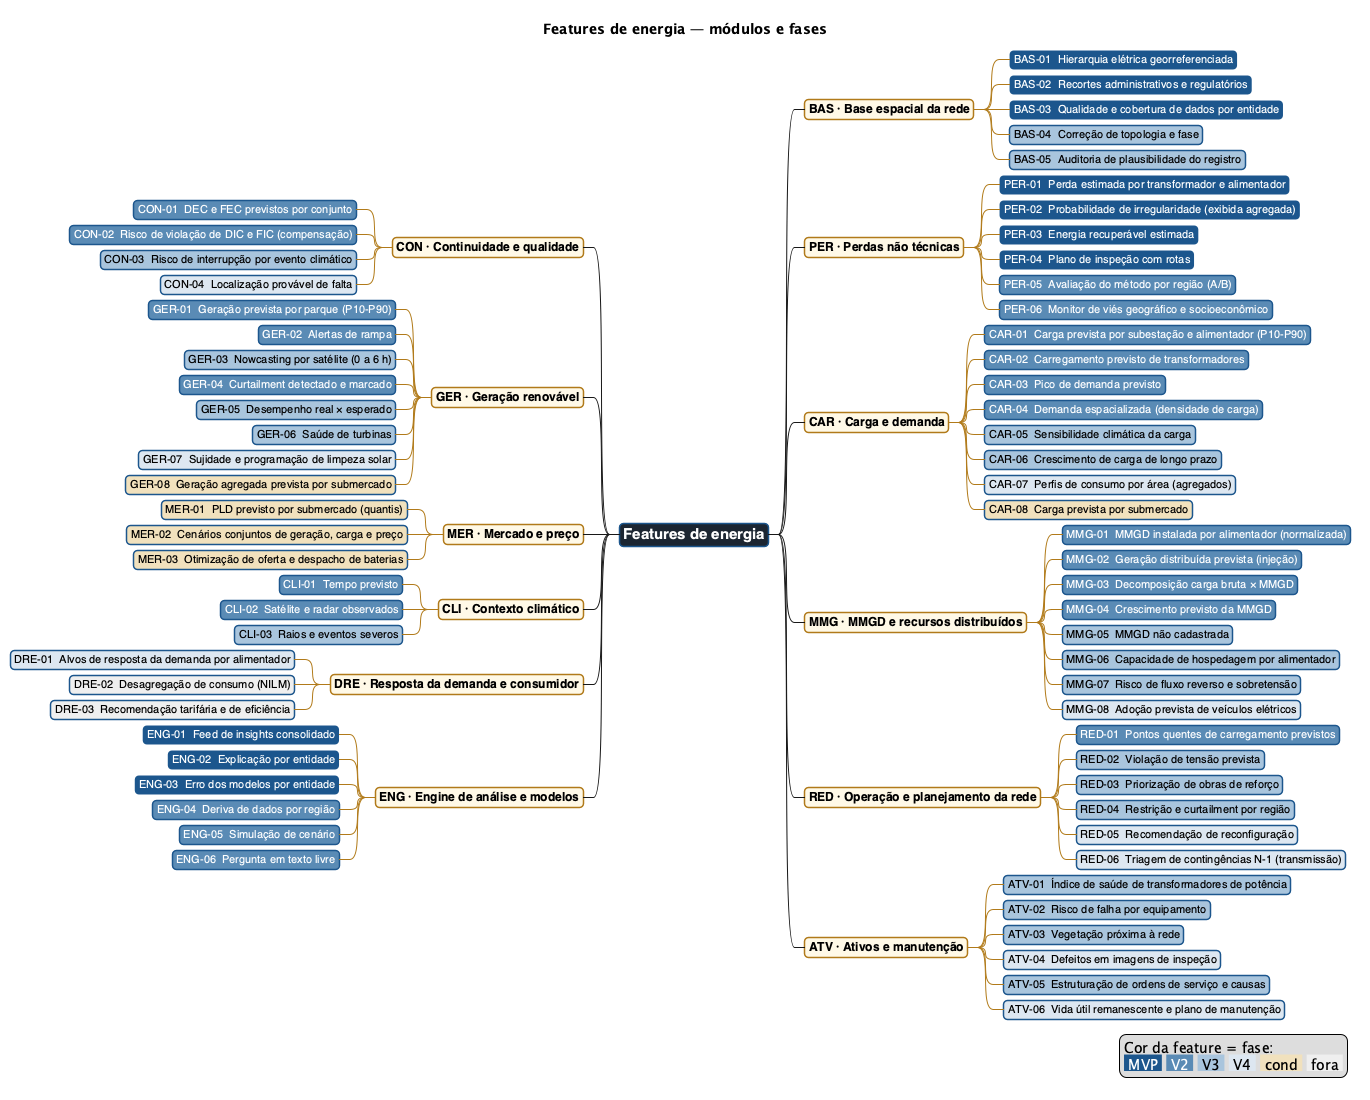
\includegraphics[width=\textwidth]{features.png}
\caption{Módulos e features, coloridos por fase.}
\label{fig:mindmap}
\end{figure}

% Gerado por features/gerar.py a partir de features/catalogo.csv. Não edite.
\begin{table}[H]\small
\caption{Features por módulo e fase.}\label{tab:fases}
\begin{tabelalarga}
\begin{tabular}{lccccccc}
\toprule
\textbf{Módulo} & \textbf{MVP} & \textbf{V2} & \textbf{V3} & \textbf{V4} & \textbf{cond} & \textbf{fora} & \textbf{Total} \\
\midrule
BAS \textperiodcentered Base espacial da rede & 3 & -- & 2 & -- & -- & -- & 5 \\
PER \textperiodcentered Perdas não técnicas & 4 & 2 & -- & -- & -- & -- & 6 \\
CAR \textperiodcentered Carga e demanda & -- & 4 & 2 & 1 & 1 & -- & 8 \\
MMG \textperiodcentered MMGD e recursos distribuídos & -- & 4 & 3 & 1 & -- & -- & 8 \\
RED \textperiodcentered Operação e planejamento da rede & -- & 1 & 3 & 2 & -- & -- & 6 \\
ATV \textperiodcentered Ativos e manutenção & -- & -- & 4 & 2 & -- & -- & 6 \\
CON \textperiodcentered Continuidade e qualidade & -- & 2 & 1 & 1 & -- & -- & 4 \\
GER \textperiodcentered Geração renovável & -- & 3 & 3 & 1 & 1 & -- & 8 \\
MER \textperiodcentered Mercado e preço & -- & -- & -- & -- & 3 & -- & 3 \\
CLI \textperiodcentered Contexto climático & -- & 2 & 1 & -- & -- & -- & 3 \\
DRE \textperiodcentered Resposta da demanda e consumidor & -- & -- & -- & 1 & -- & 2 & 3 \\
ENG \textperiodcentered Engine de análise e modelos & 3 & 3 & -- & -- & -- & -- & 6 \\
\midrule
\textbf{Total} & \textbf{10} & \textbf{21} & \textbf{19} & \textbf{9} & \textbf{5} & \textbf{2} & \textbf{66} \\
\bottomrule
\end{tabular}
\end{tabelalarga}
\end{table}

\begin{table}[H]\footnotesize
\caption{Quantas features de cada módulo servem a cada tipo de cliente.}\label{tab:clientes}
\begin{tabelalarga}
\begin{tabularx}{\linewidth}{Yccccc}
\toprule
\textbf{Módulo} & \textbf{Distribuidora} & \textbf{Transmissora} & \textbf{Gerador} & \textbf{Comercializadora} & \textbf{Consumidor} \\
\midrule
BAS \textperiodcentered Base espacial da rede & 5 & 2 & 2 & 1 & -- \\
PER \textperiodcentered Perdas não técnicas & 6 & -- & -- & -- & -- \\
CAR \textperiodcentered Carga e demanda & 7 & -- & 1 & 1 & -- \\
MMG \textperiodcentered MMGD e recursos distribuídos & 8 & -- & 1 & -- & -- \\
RED \textperiodcentered Operação e planejamento da rede & 4 & 2 & 1 & -- & -- \\
ATV \textperiodcentered Ativos e manutenção & 6 & 5 & 1 & -- & -- \\
CON \textperiodcentered Continuidade e qualidade & 4 & 1 & -- & -- & -- \\
GER \textperiodcentered Geração renovável & -- & -- & 7 & 2 & -- \\
MER \textperiodcentered Mercado e preço & -- & -- & 3 & 3 & -- \\
CLI \textperiodcentered Contexto climático & 3 & 3 & 2 & 1 & -- \\
DRE \textperiodcentered Resposta da demanda e consumidor & 1 & -- & -- & -- & 2 \\
ENG \textperiodcentered Engine de análise e modelos & 6 & 5 & 5 & 5 & -- \\
\bottomrule
\end{tabularx}
\end{tabelalarga}
\end{table}



% Leitura geral do catálogo e da pesquisa. Texto editável (não gerado).

\subsection*{Resumo do catálogo}

\begin{itemize}
  \item \textbf{66 features em 12 módulos}: 10 no MVP, 21 na V2, 19 na V3, 9
    na V4, 5 na trilha condicional e 2 fora (tabela~\ref{tab:fases}). São 59
    features comprometidas, 5 em opção e 2 descartadas. 47 têm encaixe alto com o mapa, 12
    médio e 7 baixo.
  \item \textbf{A distribuidora concentra o valor espacial}: 50 das 66
    features servem a ela (tabela~\ref{tab:clientes}). Geração renovável e
    mercado têm encaixe médio ou baixo, o que é coerente com a hipótese de cliente
    da especificação.
  \item \textbf{CON-01 e CON-02 estão na V2}: a BDGD traz DIC e FIC mensais
    por unidade. CON-02 (risco de violação de DIC e FIC) é de nível 0, tem
    encaixe alto e mede a compensação, em reais, paga pela distribuidora.
    CON-01 é pré-requisito de CON-02.
  \item \textbf{O MVP fecha o ciclo}: base (BAS-01 a 03), perdas
    (PER-01 a 04) e engine (ENG-01 a 03) cobrem feed $\rightarrow$
    diagnóstico $\rightarrow$ plano $\rightarrow$ resultado.
\end{itemize}

\subsection*{Efeitos da pesquisa sobre o catálogo}

\paragraph{1. Dados disponíveis no nível 0.} Com dado público
apenas, existem:
\begin{itemize}
  \item na BDGD: \textbf{energia mensal por alimentador, perdas técnicas e não
    técnicas por alimentador}, energia, DIC e FIC mensais por unidade, e o
    modelo elétrico que a ANEEL roda no OpenDSS;
  \item na ANEEL: \textbf{cada interrupção desde 2017 com o código do
    alimentador e da subestação}, causa e expurgo; DEC e FEC com limites;
  \item no ONS: geração por usina, constrained-off semi-horário por usina com
    razão e ponto de conexão, carga com a parcela de MMGD.
\end{itemize}
Por isso, 36 das 66 features têm versão em nível 0, entre elas PER-01 (por
alimentador), CAR-02, RED-01, CON-01 a 03, GER-01 e GER-04; quatro delas
(MMG-06, RED-01, RED-02 e ATV-02) dependem de uma feature de nível 1 ou 2. \textbf{Um
piloto em modo sombra pode ser montado antes de receber qualquer arquivo do
cliente.}

\paragraph{2. Limites do nível 0.}
\begin{itemize}
  \item \textbf{Defasagem de 8 a 20 meses} na BDGD (edição de 2025): serve para montar a rede e
    demonstrar, não para operar mês a mês.
  \item \textbf{A unidade consumidora é anonimizada} (hash) na BDGD pública.
    Ligar o dado do cliente por unidade exige a tabela de correspondência da
    distribuidora; pela rede (alimentador, transformador) a ligação tende a
    funcionar.
  \item \textbf{Unidades inconsistentes entre distribuidoras} (kWh e MWh no
    mesmo campo) e, na MMGD, injeção no lugar de geração e kW misturado com W,
    observados em duas BDGD de 2025. A normalização por distribuidora e a
    camada de qualidade (BAS-03) são necessárias.
  \item A perda não técnica das duas BDGD é compatível com \textbf{rateio
    contábil}, não com medição.
\end{itemize}

\paragraph{3. Três regras de validação atravessam o catálogo.}
\begin{itemize}
  \item \textbf{Guardar o que era conhecido em cada data}: ONS e CCEE revisam
    dados depois de publicados, e a previsão do tempo do ECMWF só fica
    disponível por 2 a 3 dias. Arquivar desde o primeiro dia é requisito.
  \item \textbf{Validar fora do espaço e do evento}: em interrupções por clima,
    divisões aleatórias inflam a estimativa de desempenho; em Essus et
    al.\ (2026), com validação espacial e temporal, muitos modelos não superam
    a linha de base.
  \item \textbf{Controlar testes múltiplos} na engine: entidades × camadas ×
    detectores exigem FDR e orçamento de alertas.
\end{itemize}

\paragraph{4. Fundamento da fração exploratória.} Revelas et al.\ (2025)
mostram que selecionar só os alvos mais prováveis leva a aprendizado
inconsistente; a seleção aleatorizada com probabilidades registradas permite
estimar, sem viés, prevalência, recall, calibração e o viés de seleção. A mesma fração alimenta PER-02, PER-05 e PER-06.

\paragraph{5. Regras regulatórias estão mudando.}
\begin{itemize}
  \item Perda não técnica calculada sobre o mercado medido desde 2025, o que
    quebra a série.
  \item Formação de preço por oferta e dois PLDs previstos para 2028 (Meta II).
  \item REN 1.098/2024 sobre inversão de fluxo da MMGD.
  \item Portaria MME 126/2026: 2\% ao ano de medidores inteligentes,
    priorizando perdas.
  \item Proposta de Tarifa Branca automática.
\end{itemize}
Cada uma é um ponto de deriva a monitorar (ENG-04).

\paragraph{6. Licenças a observar.} BDGD em ODbL (compartilhamento pela mesma
licença em bases derivadas públicas: consultar o jurídico); ECMWF em CC-BY com
atribuição no mapa; \emph{alibi-detect} em Business Source License, com
restrição comercial.

\subsection*{A trilha condicional}

Cinco features --- MER-01 a MER-03, CAR-08 e GER-08 --- saíram do roadmap
faseado para a trilha \textbf{cond}. Não são features descartadas: são uma
opção sobre a questão de cliente-alvo que a especificação deixa em aberto
(distribuidora, ou gerador e comercializadora). Enquanto essa questão não for
respondida, elas não recebem fase.

A retirada não afeta as demais: formam uma subárvore isolada
---~CAR-08 e GER-08 $\rightarrow$ MER-01 $\rightarrow$ MER-02 $\rightarrow$
MER-03~--- e \textbf{nada fora dela depende de nenhuma das cinco}. As
dependências externas da subárvore são CLI-01 (de CAR-08) e GER-01 (de GER-08
e MER-02), features que permanecem no roadmap.

Três observações pesaram na decisão:
\begin{itemize}
  \item \textbf{É a parte do gerador em que o mapa não ajuda.} As cinco têm
    encaixe baixo, e o preço por submercado ocupa quatro polígonos. Se a trilha
    de gerador for tomada, a âncora espacial é \textbf{RED-04} (restrição e
    curtailment por região): encaixe alto, nível 0, sem dependências, e já
    sustentada pelo constrained-off semi-horário do ONS.
  \item \textbf{A premissa de MER-03 só existe a partir de 2028.} Oferta só faz sentido com
    o modelo híbrido do Projeto Meta II, e o primeiro leilão de baterias
    (Portaria MME 136/2026) remunera disponibilidade, não arbitragem livre.
  \item \textbf{A continuidade da fonte não é garantida.} O portal de dados
    abertos da CCEE tem bloqueio de aplicação; o endpoint CKAN funcionou em
    23/09/2026.
\end{itemize}

\subsection*{Cadeias de dependência}

As dependências do catálogo definem a ordem de construção. As principais do roadmap faseado:
\begin{itemize}
  \item BAS-01 $\rightarrow$ PER-01, PER-02 $\rightarrow$ PER-03 $\rightarrow$
    PER-04 $\rightarrow$ PER-05, PER-06 (o MVP e sua avaliação);
  \item MMG-01 $\rightarrow$ MMG-02 $\rightarrow$ MMG-03, MMG-06, MMG-07;
  \item CAR-01, CAR-02 $\rightarrow$ RED-01 $\rightarrow$ RED-03, DRE-01;
  \item ATV-03 $\rightarrow$ CON-03, e ATV-01, ATV-02 $\rightarrow$ ATV-06.
\end{itemize}

\subsection*{Pendências de verificação}

\begin{enumerate}
  \item Manual de Instruções da BDGD (não baixado): definição oficial de
    energia e perdas na CTMT, energia das unidades geradoras (injeção ou
    geração), unidade da potência instalada.
  \item Se o código de conjunto da BDGD casa com o dos indicadores de DEC e
    FEC.
  \item Se a distribuidora consegue reproduzir o hash do código da unidade.
  \item Unidade do valor nas curvas típicas CTR.
  \item Existência de obrigação regulatória de publicar capacidade de
    hospedagem.
  \item Consulta jurídica sobre a ODbL em camadas derivadas.
\end{enumerate}


% ===========================================================================
% ===========================================================================

\begin{landscape}
\part{Catálogo}
\section{Catálogo por módulo}
% Gerado por features/gerar.py a partir de features/catalogo.csv. Não edite.
\subsection*{BAS \textperiodcentered{} Base espacial da rede}
\addcontentsline{toc}{subsection}{BAS \textperiodcentered{} Base espacial da rede}
\label{cat:BAS}
{\footnotesize\setlength{\tabcolsep}{3pt}
\begin{longtable}{@{}P{1.35cm}P{4.1cm}P{1.3cm}P{3.1cm}P{3.7cm}C{0.6cm}P{3.6cm}P{3.3cm}P{1.1cm}P{0.9cm}P{1.1cm}@{}}
\toprule
\textbf{ID} & \textbf{Feature} & \textbf{Tipo} & \textbf{Entidade} & \textbf{Dados} & \textbf{Nív.} & \textbf{Modelo} & \textbf{Insight / decisão} & \textbf{Cliente} & \textbf{Mapa} & \textbf{Fase} \\
\midrule\endhead
\textbf{BAS-01} & Hierarquia elétrica georreferenciada & base & concessão, SE, alimentador, transformador, UC & BDGD (geodatabase anual, ODbL, 8 a 20 meses de defasagem) & 0 & ETL, grafo por pontos de conexão, normalização de unidades por distribuidora & navegar, selecionar & D & \encaixe{3} & \colorbox{fMVP}{\scriptsize \textcolor{white}{\textbf{MVP}}} \\
\textbf{BAS-02} & Recortes administrativos e regulatórios & base & estado, município, setor censitário, conjunto elétrico & IBGE (malhas), ANEEL (conjuntos) & 0 & ETL & cruzar, filtrar & D T G & \encaixe{3} & \colorbox{fMVP}{\scriptsize \textcolor{white}{\textbf{MVP}}} \\
\textbf{BAS-03} & Qualidade e cobertura de dados por entidade\newline{\color{black!55}\scriptsize depende: BAS-01} & camada & todas & todas as fontes ingeridas & 0 & regras de completude e validade & lacuna de dados / acionar fonte, ressalvar camada & D T G C & \encaixe{3} & \colorbox{fMVP}{\scriptsize \textcolor{white}{\textbf{MVP}}} \\
\textbf{BAS-04} & Correção de topologia e fase\newline{\color{black!55}\scriptsize depende: BAS-01} & camada & UC agregada, transformador & medição inteligente (tensão), BDGD & 3 & correlação de séries de tensão, agrupamento & divergência cadastro $\times$ medição / corrigir cadastro & D & \encaixe{3} & \colorbox{fV3}{\scriptsize \textbf{V3}} \\
\textbf{BAS-05} & Auditoria de plausibilidade do registro\newline{\color{black!55}\scriptsize depende: BAS-01} & insight & UC agregada, usina & BDGD, registro de MMGD da ANEEL, reanálise (NASA POWER) & 0 & teto físico (modelo de recurso solar), regras & divergência modelo $\times$ registro / corrigir cadastro, fiscalizar & D & \encaixe{3} & \colorbox{fV3}{\scriptsize \textbf{V3}} \\
\bottomrule
\end{longtable}}

\subsection*{PER \textperiodcentered{} Perdas não técnicas}
\addcontentsline{toc}{subsection}{PER \textperiodcentered{} Perdas não técnicas}
\label{cat:PER}
{\footnotesize\setlength{\tabcolsep}{3pt}
\begin{longtable}{@{}P{1.35cm}P{4.1cm}P{1.3cm}P{3.1cm}P{3.7cm}C{0.6cm}P{3.6cm}P{3.3cm}P{1.1cm}P{0.9cm}P{1.1cm}@{}}
\toprule
\textbf{ID} & \textbf{Feature} & \textbf{Tipo} & \textbf{Entidade} & \textbf{Dados} & \textbf{Nív.} & \textbf{Modelo} & \textbf{Insight / decisão} & \textbf{Cliente} & \textbf{Mapa} & \textbf{Fase} \\
\midrule\endhead
\textbf{PER-01} & Perda estimada por transformador e alimentador\newline{\color{black!55}\scriptsize depende: BAS-01} & camada & transformador, alimentador & BDGD (energia do alimentador, perdas técnicas e não técnicas, energia por unidade), faturamento do cliente, medição no transformador quando houver & 0 & balanço energético (energia do alimentador -- soma das unidades -- técnica), técnica no OpenDSS, rateio hierárquico bayesiano entre transformadores & anomalia espacial, mudança entre ciclos / selecionar alvos & D & \encaixe{3} & \colorbox{fMVP}{\scriptsize \textcolor{white}{\textbf{MVP}}} \\
\textbf{PER-02} & Probabilidade de irregularidade (exibida agregada)\newline{\color{black!55}\scriptsize depende: BAS-01} & camada & UC agregada por transformador & faturamento, cadastro, histórico de inspeções & 1 & gradient boosting com vizinhança, peso inverso da propensão de inspeção, PU learning com propensão (SAR) & concentração / compor alvos do plano & D & \encaixe{3} & \colorbox{fMVP}{\scriptsize \textcolor{white}{\textbf{MVP}}} \\
\textbf{PER-03} & Energia recuperável estimada\newline{\color{black!55}\scriptsize depende: PER-01, PER-02} & camada & transformador, alimentador, plano & PER-01, PER-02, consumo & 1 & probabilidade $\times$ energia desviada estimada & ranking por valor / priorizar & D & \encaixe{3} & \colorbox{fMVP}{\scriptsize \textcolor{white}{\textbf{MVP}}} \\
\textbf{PER-04} & Plano de inspeção com rotas\newline{\color{black!55}\scriptsize depende: PER-02, PER-03} & decisão & seleção & PER-02, PER-03, base operacional, restrição do usuário & 1 & team orienteering problem (OR-Tools) com fração exploratória sorteada e probabilidades registradas & aprovar e enviar ao campo & D & \encaixe{3} & \colorbox{fMVP}{\scriptsize \textcolor{white}{\textbf{MVP}}} \\
\textbf{PER-05} & Avaliação do método por região (A/B)\newline{\color{black!55}\scriptsize depende: PER-04} & insight & região, lote & resultados de inspeção & 1 & teste A/B, precisão no topo da lista & desempenho do método / ajustar política de inspeção & D & \encaixe{2} & \colorbox{fV2}{\scriptsize \textcolor{white}{\textbf{V2}}} \\
\textbf{PER-06} & Monitor de viés geográfico e socioeconômico\newline{\color{black!55}\scriptsize depende: PER-04} & insight & setor censitário, município & inspeções, IBGE & 1 & taxa de indicação $\times$ taxa confirmada por recorte & concentração injustificada / rever critérios & D & \encaixe{3} & \colorbox{fV2}{\scriptsize \textcolor{white}{\textbf{V2}}} \\
\bottomrule
\end{longtable}}

\subsection*{CAR \textperiodcentered{} Carga e demanda}
\addcontentsline{toc}{subsection}{CAR \textperiodcentered{} Carga e demanda}
\label{cat:CAR}
{\footnotesize\setlength{\tabcolsep}{3pt}
\begin{longtable}{@{}P{1.35cm}P{4.1cm}P{1.3cm}P{3.1cm}P{3.7cm}C{0.6cm}P{3.6cm}P{3.3cm}P{1.1cm}P{0.9cm}P{1.1cm}@{}}
\toprule
\textbf{ID} & \textbf{Feature} & \textbf{Tipo} & \textbf{Entidade} & \textbf{Dados} & \textbf{Nív.} & \textbf{Modelo} & \textbf{Insight / decisão} & \textbf{Cliente} & \textbf{Mapa} & \textbf{Fase} \\
\midrule\endhead
\textbf{CAR-01} & Carga prevista por subestação e alimentador (P10--P90)\newline{\color{black!55}\scriptsize depende: BAS-01, CLI-01} & camada & SE, alimentador & medição de SE e alimentador, previsão do tempo, calendário & 2 & gradient boosting quantílico ou TFT, reconciliação hierárquica (MinT) & tendência e limiar / programar operação & D & \encaixe{3} & \colorbox{fV2}{\scriptsize \textcolor{white}{\textbf{V2}}} \\
\textbf{CAR-02} & Carregamento previsto de transformadores\newline{\color{black!55}\scriptsize depende: BAS-01} & camada & transformador & BDGD (energia mensal e tipologia por unidade), curvas típicas CTR (ANEEL), medição no transformador quando houver & 0 & método regulatório (energia $\times$ curva típica no OpenDSS) calibrado em transformadores medidos & limiar (sobrecarga) / remanejar, trocar transformador & D & \encaixe{3} & \colorbox{fV2}{\scriptsize \textcolor{white}{\textbf{V2}}} \\
\textbf{CAR-03} & Pico de demanda previsto\newline{\color{black!55}\scriptsize depende: CAR-01} & camada & alimentador, transformador & séries medidas & 2 & previsão probabilística de pico por simulação com clima reamostrado, valores extremos & tendência e limiar / reforço, gestão de pico & D & \encaixe{3} & \colorbox{fV2}{\scriptsize \textcolor{white}{\textbf{V2}}} \\
\textbf{CAR-04} & Demanda espacializada (densidade de carga)\newline{\color{black!55}\scriptsize depende: BAS-02} & camada & setor censitário, grade & BDGD, IBGE, Open Buildings 2.5D, luzes noturnas (NASA) & 0 & dasimétrico: consumo $\times$ edificações, população e luzes noturnas & concentração, mudança / planejar expansão & D & \encaixe{3} & \colorbox{fV2}{\scriptsize \textcolor{white}{\textbf{V2}}} \\
\textbf{CAR-05} & Sensibilidade climática da carga\newline{\color{black!55}\scriptsize depende: CAR-01} & camada & alimentador, SE & medição, reanálise, previsão do tempo & 2 & regressão por partes com graus-dia, GAM & limiar em onda de calor / preparar operação & D & \encaixe{2} & \colorbox{fV3}{\scriptsize \textbf{V3}} \\
\textbf{CAR-06} & Crescimento de carga de longo prazo\newline{\color{black!55}\scriptsize depende: CAR-04} & camada & município, alimentador & consumo histórico, IBGE, EPE (PDE) & 0 & modelos estruturais com cenários & tendência / plano de expansão & D & \encaixe{3} & \colorbox{fV3}{\scriptsize \textbf{V3}} \\
\textbf{CAR-07} & Perfis de consumo por área (agregados)\newline{\color{black!55}\scriptsize depende: BAS-01} & camada & transformador, setor censitário & medição inteligente ou faturamento & 3 & agrupamento de curvas de carga & mudança de perfil / tarifas, campanhas & D & \encaixe{2} & \colorbox{fV4}{\scriptsize \textbf{V4}} \\
\textbf{CAR-08} & Carga prevista por submercado\newline{\color{black!55}\scriptsize depende: CLI-01} & camada & submercado & ONS (carga verificada e programada), previsão do tempo & 0 & gradient boosting ou TFT & tendência / contratação & C G & \encaixe{1} & \colorbox{fCond}{\scriptsize \textbf{cond}} \\
\bottomrule
\end{longtable}}

\subsection*{MMG \textperiodcentered{} MMGD e recursos distribuídos}
\addcontentsline{toc}{subsection}{MMG \textperiodcentered{} MMGD e recursos distribuídos}
\label{cat:MMG}
{\footnotesize\setlength{\tabcolsep}{3pt}
\begin{longtable}{@{}P{1.35cm}P{4.1cm}P{1.3cm}P{3.1cm}P{3.7cm}C{0.6cm}P{3.6cm}P{3.3cm}P{1.1cm}P{0.9cm}P{1.1cm}@{}}
\toprule
\textbf{ID} & \textbf{Feature} & \textbf{Tipo} & \textbf{Entidade} & \textbf{Dados} & \textbf{Nív.} & \textbf{Modelo} & \textbf{Insight / decisão} & \textbf{Cliente} & \textbf{Mapa} & \textbf{Fase} \\
\midrule\endhead
\textbf{MMG-01} & MMGD instalada por alimentador (normalizada)\newline{\color{black!55}\scriptsize depende: BAS-01} & contexto & alimentador, transformador & registro de MMGD da ANEEL (mensal), BDGD & 0 & junção registro $\times$ BDGD, normalização de unidades, conversão módulo (CC) para inversor (CA) & concentração & D & \encaixe{3} & \colorbox{fV2}{\scriptsize \textcolor{white}{\textbf{V2}}} \\
\textbf{MMG-02} & Geração distribuída prevista (injeção)\newline{\color{black!55}\scriptsize depende: MMG-01, CLI-01} & camada & alimentador, SE & MMG-01, previsão do tempo, satélite, medição quando houver & 0 & irradiância prevista $\times$ capacidade instalada, calibrada & rampa, limiar de fluxo reverso / operar a rede & D & \encaixe{3} & \colorbox{fV2}{\scriptsize \textcolor{white}{\textbf{V2}}} \\
\textbf{MMG-03} & Decomposição carga bruta $\times$ MMGD\newline{\color{black!55}\scriptsize depende: CAR-01, MMG-02} & camada & alimentador, SE & CAR-01, MMG-02 & 2 & carga líquida = bruta -- MMGD, modelos separados & curva do pato acentuada / planejar operação & D & \encaixe{3} & \colorbox{fV2}{\scriptsize \textcolor{white}{\textbf{V2}}} \\
\textbf{MMG-04} & Crescimento previsto da MMGD\newline{\color{black!55}\scriptsize depende: MMG-01} & camada & alimentador, município & registro de MMGD da ANEEL, IBGE, PDE 2035 & 0 & Bass hierárquico com covariáveis espaciais, referência EPE 4MD (epe4md) & tendência / planejar reforço & D & \encaixe{3} & \colorbox{fV2}{\scriptsize \textcolor{white}{\textbf{V2}}} \\
\textbf{MMG-05} & MMGD não cadastrada\newline{\color{black!55}\scriptsize depende: MMG-01} & insight & transformador, UC agregada & faturamento ou medição inteligente, imagens & 1 & anomalia no perfil de consumo, detecção em imagem de telhados & divergência modelo $\times$ registro / regularizar & D & \encaixe{3} & \colorbox{fV3}{\scriptsize \textbf{V3}} \\
\textbf{MMG-06} & Capacidade de hospedagem por alimentador\newline{\color{black!55}\scriptsize depende: MMG-02, CAR-01} & camada & alimentador & modelo elétrico da BDGD, MMG-02, CAR-01 & 0 & surrogate de fluxo de potência de distribuição sobre cenários & limiar (sem folga) / aprovar ou negar conexões, reforçar & D G & \encaixe{3} & \colorbox{fV3}{\scriptsize \textbf{V3}} \\
\textbf{MMG-07} & Risco de fluxo reverso e sobretensão\newline{\color{black!55}\scriptsize depende: MMG-02, CAR-02} & insight & alimentador, transformador & MMG-02, CAR-02 & 0 & limiar de injeção prevista sobre carga mínima & limiar / ajustar tap, reforçar & D & \encaixe{3} & \colorbox{fV3}{\scriptsize \textbf{V3}} \\
\textbf{MMG-08} & Adoção prevista de veículos elétricos\newline{\color{black!55}\scriptsize depende: CAR-06} & camada & município, alimentador & frota por município (Senatran), IBGE & 0 & modelo de difusão com renda e frota & tendência / planejar reforço & D & \encaixe{3} & \colorbox{fV4}{\scriptsize \textbf{V4}} \\
\bottomrule
\end{longtable}}

\subsection*{RED \textperiodcentered{} Operação e planejamento da rede}
\addcontentsline{toc}{subsection}{RED \textperiodcentered{} Operação e planejamento da rede}
\label{cat:RED}
{\footnotesize\setlength{\tabcolsep}{3pt}
\begin{longtable}{@{}P{1.35cm}P{4.1cm}P{1.3cm}P{3.1cm}P{3.7cm}C{0.6cm}P{3.6cm}P{3.3cm}P{1.1cm}P{0.9cm}P{1.1cm}@{}}
\toprule
\textbf{ID} & \textbf{Feature} & \textbf{Tipo} & \textbf{Entidade} & \textbf{Dados} & \textbf{Nív.} & \textbf{Modelo} & \textbf{Insight / decisão} & \textbf{Cliente} & \textbf{Mapa} & \textbf{Fase} \\
\midrule\endhead
\textbf{RED-01} & Pontos quentes de carregamento previstos\newline{\color{black!55}\scriptsize depende: CAR-01, CAR-02} & camada & alimentador, transformador, SE & BDGD convertida para OpenDSS, CAR-01, CAR-02 & 0 & quantis do pico agregados pela topologia, fluxo confirmado no OpenDSS & limiar / remanejar carga & D & \encaixe{3} & \colorbox{fV2}{\scriptsize \textcolor{white}{\textbf{V2}}} \\
\textbf{RED-02} & Violação de tensão prevista\newline{\color{black!55}\scriptsize depende: CAR-01, MMG-02} & camada & alimentador, barra & modelo elétrico da BDGD (bdgd2opendss), carga e MMGD previstas & 0 & surrogate de fluxo de potência (GNN), verificado por solver & limiar / ajustar regulação & D & \encaixe{3} & \colorbox{fV3}{\scriptsize \textbf{V3}} \\
\textbf{RED-03} & Priorização de obras de reforço\newline{\color{black!55}\scriptsize depende: RED-01, CAR-06, MMG-06, CON-01, CON-02} & decisão & alimentador, SE & RED-01, CAR-06, MMG-06 & 1 & otimização sob orçamento: risco $\times$ custo & plano de investimentos & D & \encaixe{3} & \colorbox{fV3}{\scriptsize \textbf{V3}} \\
\textbf{RED-04} & Restrição e curtailment por região & camada & SE, barra & ONS constrained-off por usina (semi-horário, com razão e ponto de conexão) & 0 & modelo de probabilidade de restrição por região & concentração / localizar nova geração & G T & \encaixe{3} & \colorbox{fV3}{\scriptsize \textbf{V3}} \\
\textbf{RED-05} & Recomendação de reconfiguração\newline{\color{black!55}\scriptsize depende: RED-02} & decisão & alimentador & modelo elétrico, carga prevista & 2 & GNN e otimização, verificado por solver & chaveamento & D & \encaixe{2} & \colorbox{fV4}{\scriptsize \textbf{V4}} \\
\textbf{RED-06} & Triagem de contingências N-1 (transmissão)\newline{\color{black!55}\scriptsize depende: RED-02} & camada & linha, SE & modelo da rede do cliente, previsões & 2 & surrogate GNN com confirmação por fluxo de potência completo & limiar / ações corretivas & T & \encaixe{2} & \colorbox{fV4}{\scriptsize \textbf{V4}} \\
\bottomrule
\end{longtable}}

\subsection*{ATV \textperiodcentered{} Ativos e manutenção}
\addcontentsline{toc}{subsection}{ATV \textperiodcentered{} Ativos e manutenção}
\label{cat:ATV}
{\footnotesize\setlength{\tabcolsep}{3pt}
\begin{longtable}{@{}P{1.35cm}P{4.1cm}P{1.3cm}P{3.1cm}P{3.7cm}C{0.6cm}P{3.6cm}P{3.3cm}P{1.1cm}P{0.9cm}P{1.1cm}@{}}
\toprule
\textbf{ID} & \textbf{Feature} & \textbf{Tipo} & \textbf{Entidade} & \textbf{Dados} & \textbf{Nív.} & \textbf{Modelo} & \textbf{Insight / decisão} & \textbf{Cliente} & \textbf{Mapa} & \textbf{Fase} \\
\midrule\endhead
\textbf{ATV-01} & Índice de saúde de transformadores de potência\newline{\color{black!55}\scriptsize depende: BAS-01} & camada & transformador de potência (SE) & laudos de óleo (DGA), ensaios, carregamento & 1 & gradient boosting sobre gases dissolvidos, carregamento e idade & mudança, limiar / inspecionar, manter & D T & \encaixe{3} & \colorbox{fV3}{\scriptsize \textbf{V3}} \\
\textbf{ATV-02} & Risco de falha por equipamento\newline{\color{black!55}\scriptsize depende: ATV-05} & camada & equipamento, alimentador & BDGD, interrupções por evento (ANEEL), ordens de serviço do cliente, clima & 0 & random survival forest, contagem por km & concentração / manutenção preventiva & D & \encaixe{3} & \colorbox{fV3}{\scriptsize \textbf{V3}} \\
\textbf{ATV-03} & Vegetação próxima à rede\newline{\color{black!55}\scriptsize depende: BAS-01} & camada & trecho de alimentador, linha & altura de dossel (Lang 10 m, Meta 1 m), Sentinel-2, LiDAR do cliente & 0 & mapas globais de altura de dossel, segmentação e regressão de altura & concentração / programa de poda & D T & \encaixe{3} & \colorbox{fV3}{\scriptsize \textbf{V3}} \\
\textbf{ATV-04} & Defeitos em imagens de inspeção & camada & estrutura, equipamento & imagens de drone & 1 & detecção de objetos (YOLO, DETR) & concentração / ordem de serviço & D T G & \encaixe{3} & \colorbox{fV4}{\scriptsize \textbf{V4}} \\
\textbf{ATV-05} & Estruturação de ordens de serviço e causas & base & equipamento, alimentador & ordens de serviço em texto & 1 & extração com modelo de linguagem & concentração de causa & D T & \encaixe{2} & \colorbox{fV3}{\scriptsize \textbf{V3}} \\
\textbf{ATV-06} & Vida útil remanescente e plano de manutenção\newline{\color{black!55}\scriptsize depende: ATV-01, ATV-02} & decisão & equipamento & ATV-01, ATV-02 & 1 & sobrevivência e otimização sob orçamento e equipes & plano de manutenção & D T & \encaixe{3} & \colorbox{fV4}{\scriptsize \textbf{V4}} \\
\bottomrule
\end{longtable}}

\subsection*{CON \textperiodcentered{} Continuidade e qualidade}
\addcontentsline{toc}{subsection}{CON \textperiodcentered{} Continuidade e qualidade}
\label{cat:CON}
{\footnotesize\setlength{\tabcolsep}{3pt}
\begin{longtable}{@{}P{1.35cm}P{4.1cm}P{1.3cm}P{3.1cm}P{3.7cm}C{0.6cm}P{3.6cm}P{3.3cm}P{1.1cm}P{0.9cm}P{1.1cm}@{}}
\toprule
\textbf{ID} & \textbf{Feature} & \textbf{Tipo} & \textbf{Entidade} & \textbf{Dados} & \textbf{Nív.} & \textbf{Modelo} & \textbf{Insight / decisão} & \textbf{Cliente} & \textbf{Mapa} & \textbf{Fase} \\
\midrule\endhead
\textbf{CON-01} & DEC e FEC previstos por conjunto\newline{\color{black!55}\scriptsize depende: BAS-02} & camada & conjunto elétrico & DEC e FEC por conjunto (ANEEL), interrupções por evento com código do alimentador (ANEEL, desde 2017), clima & 0 & séries temporais com clima & limiar contra meta regulatória / ações de melhoria & D & \encaixe{3} & \colorbox{fV2}{\scriptsize \textcolor{white}{\textbf{V2}}} \\
\textbf{CON-02} & Risco de violação de DIC e FIC (compensação)\newline{\color{black!55}\scriptsize depende: CON-01} & camada & alimentador, transformador (agregado) & DIC e FIC mensais por unidade na BDGD, interrupções por evento (ANEEL), TUSD & 0 & simulação de DIC, FIC e DMIC por unidade e regras de compensação do PRODIST & ranking por valor / priorizar ações & D & \encaixe{3} & \colorbox{fV2}{\scriptsize \textcolor{white}{\textbf{V2}}} \\
\textbf{CON-03} & Risco de interrupção por evento climático\newline{\color{black!55}\scriptsize depende: CLI-01, CLI-03, ATV-03} & camada & trecho de alimentador, linha & interrupções por evento com causa (ANEEL), previsão do tempo, raios (GLM aberto ou BrasilDAT), ATV-03 & 0 & clima previsto $\times$ vulnerabilidade (vegetação, idade) & limiar / pré-posicionar equipes & D T & \encaixe{3} & \colorbox{fV3}{\scriptsize \textbf{V3}} \\
\textbf{CON-04} & Localização provável de falta\newline{\color{black!55}\scriptsize depende: BAS-01} & camada & trecho de alimentador & eventos de religadores, medição inteligente, chamadas & 3 & classificação sobre religadores, medição e chamadas & despachar equipe & D & \encaixe{3} & \colorbox{fV4}{\scriptsize \textbf{V4}} \\
\bottomrule
\end{longtable}}

\subsection*{GER \textperiodcentered{} Geração renovável}
\addcontentsline{toc}{subsection}{GER \textperiodcentered{} Geração renovável}
\label{cat:GER}
{\footnotesize\setlength{\tabcolsep}{3pt}
\begin{longtable}{@{}P{1.35cm}P{4.1cm}P{1.3cm}P{3.1cm}P{3.7cm}C{0.6cm}P{3.6cm}P{3.3cm}P{1.1cm}P{0.9cm}P{1.1cm}@{}}
\toprule
\textbf{ID} & \textbf{Feature} & \textbf{Tipo} & \textbf{Entidade} & \textbf{Dados} & \textbf{Nív.} & \textbf{Modelo} & \textbf{Insight / decisão} & \textbf{Cliente} & \textbf{Mapa} & \textbf{Fase} \\
\midrule\endhead
\textbf{GER-01} & Geração prevista por parque (P10--P90)\newline{\color{black!55}\scriptsize depende: CLI-01} & camada & parque & geração por usina do ONS (pública), SCADA do parque, previsão do tempo & 0 & gradient boosting ou TFT sobre previsão do tempo, zero-shot no onboarding & tendência / programação e declaração & G C & \encaixe{2} & \colorbox{fV2}{\scriptsize \textcolor{white}{\textbf{V2}}} \\
\textbf{GER-02} & Alertas de rampa\newline{\color{black!55}\scriptsize depende: GER-01} & insight & parque, região & GER-01 & 1 & limiar na trajetória prevista & tendência e limiar / ajustar oferta & G & \encaixe{2} & \colorbox{fV2}{\scriptsize \textcolor{white}{\textbf{V2}}} \\
\textbf{GER-03} & Nowcasting por satélite (0 a 6 h)\newline{\color{black!55}\scriptsize depende: CLI-02} & camada & parque, região & GOES-19 & 0 & U-Net sobre índice de nuvem, difusão latente (SHADECast) & mudança / ajuste intradiário & G & \encaixe{3} & \colorbox{fV3}{\scriptsize \textbf{V3}} \\
\textbf{GER-04} & Curtailment detectado e marcado\newline{\color{black!55}\scriptsize depende: GER-01} & camada & parque & ONS constrained-off por usina, SCADA & 0 & regras e modelo de potência disponível & concentração / contestar, limpar treino & G & \encaixe{2} & \colorbox{fV2}{\scriptsize \textcolor{white}{\textbf{V2}}} \\
\textbf{GER-05} & Desempenho real $\times$ esperado\newline{\color{black!55}\scriptsize depende: GER-01} & insight & parque, turbina, bloco solar & SCADA, recurso & 1 & modelo de comportamento normal & divergência modelo $\times$ registro / inspecionar & G & \encaixe{2} & \colorbox{fV3}{\scriptsize \textbf{V3}} \\
\textbf{GER-06} & Saúde de turbinas & camada & turbina & SCADA de turbina & 1 & modelo de comportamento normal sobre temperaturas e vibração & mudança / manutenção & G & \encaixe{3} & \colorbox{fV3}{\scriptsize \textbf{V3}} \\
\textbf{GER-07} & Sujidade e programação de limpeza solar\newline{\color{black!55}\scriptsize depende: GER-05} & decisão & parque, bloco solar & SCADA, chuva & 1 & perda por sujidade estimada $\times$ custo de limpeza & limiar / programar limpeza & G & \encaixe{2} & \colorbox{fV4}{\scriptsize \textbf{V4}} \\
\textbf{GER-08} & Geração agregada prevista por submercado\newline{\color{black!55}\scriptsize depende: GER-01} & camada & submercado & GER-01, ONS & 0 & agregação de previsões & tendência / posição comercial & C & \encaixe{1} & \colorbox{fCond}{\scriptsize \textbf{cond}} \\
\bottomrule
\end{longtable}}

\subsection*{MER \textperiodcentered{} Mercado e preço}
\addcontentsline{toc}{subsection}{MER \textperiodcentered{} Mercado e preço}
\label{cat:MER}
{\footnotesize\setlength{\tabcolsep}{3pt}
\begin{longtable}{@{}P{1.35cm}P{4.1cm}P{1.3cm}P{3.1cm}P{3.7cm}C{0.6cm}P{3.6cm}P{3.3cm}P{1.1cm}P{0.9cm}P{1.1cm}@{}}
\toprule
\textbf{ID} & \textbf{Feature} & \textbf{Tipo} & \textbf{Entidade} & \textbf{Dados} & \textbf{Nív.} & \textbf{Modelo} & \textbf{Insight / decisão} & \textbf{Cliente} & \textbf{Mapa} & \textbf{Fase} \\
\midrule\endhead
\textbf{MER-01} & PLD previsto por submercado (quantis)\newline{\color{black!55}\scriptsize depende: CAR-08, GER-08} & camada & submercado & CCEE PLD horário (CSV anual, CC-BY), decks NEWAVE/DECOMP/DESSEM, ONS & 0 & gradient boosting ou emulação do DESSEM & tendência / posição comercial & C G & \encaixe{1} & \colorbox{fCond}{\scriptsize \textbf{cond}} \\
\textbf{MER-02} & Cenários conjuntos de geração, carga e preço\newline{\color{black!55}\scriptsize depende: MER-01, CAR-08, GER-01} & camada & submercado, parque & GER-01, CAR-08, MER-01 & 0 & cópulas sobre previsões marginais & análise de risco & C G & \encaixe{1} & \colorbox{fCond}{\scriptsize \textbf{cond}} \\
\textbf{MER-03} & Otimização de oferta e despacho de baterias\newline{\color{black!55}\scriptsize depende: MER-02} & decisão & parque, bateria & MER-02 & 1 & otimização estocástica sobre cenários & oferta, despacho & G C & \encaixe{1} & \colorbox{fCond}{\scriptsize \textbf{cond}} \\
\bottomrule
\end{longtable}}

\subsection*{CLI \textperiodcentered{} Contexto climático}
\addcontentsline{toc}{subsection}{CLI \textperiodcentered{} Contexto climático}
\label{cat:CLI}
{\footnotesize\setlength{\tabcolsep}{3pt}
\begin{longtable}{@{}P{1.35cm}P{4.1cm}P{1.3cm}P{3.1cm}P{3.7cm}C{0.6cm}P{3.6cm}P{3.3cm}P{1.1cm}P{0.9cm}P{1.1cm}@{}}
\toprule
\textbf{ID} & \textbf{Feature} & \textbf{Tipo} & \textbf{Entidade} & \textbf{Dados} & \textbf{Nív.} & \textbf{Modelo} & \textbf{Insight / decisão} & \textbf{Cliente} & \textbf{Mapa} & \textbf{Fase} \\
\midrule\endhead
\textbf{CLI-01} & Tempo previsto & contexto & grade & ECMWF Open Data (CC-BY), GFS, CPTEC/INPE, INMET & 0 & previsão numérica do tempo com pós-processamento por entidade & -- & D T G C & \encaixe{3} & \colorbox{fV2}{\scriptsize \textcolor{white}{\textbf{V2}}} \\
\textbf{CLI-02} & Satélite e radar observados & contexto & grade & GOES-19 (ABI), radar REDEMET e CEMADEN & 0 & nowcasting de precipitação (pysteps) & -- & D T G & \encaixe{3} & \colorbox{fV2}{\scriptsize \textcolor{white}{\textbf{V2}}} \\
\textbf{CLI-03} & Raios e eventos severos & contexto & grade & BrasilDAT (ELAT/INPE, sob contrato) ou GLM do GOES-19 (aberto) & 0 & -- & -- & D T & \encaixe{3} & \colorbox{fV3}{\scriptsize \textbf{V3}} \\
\bottomrule
\end{longtable}}

\subsection*{DRE \textperiodcentered{} Resposta da demanda e consumidor}
\addcontentsline{toc}{subsection}{DRE \textperiodcentered{} Resposta da demanda e consumidor}
\label{cat:DRE}
{\footnotesize\setlength{\tabcolsep}{3pt}
\begin{longtable}{@{}P{1.35cm}P{4.1cm}P{1.3cm}P{3.1cm}P{3.7cm}C{0.6cm}P{3.6cm}P{3.3cm}P{1.1cm}P{0.9cm}P{1.1cm}@{}}
\toprule
\textbf{ID} & \textbf{Feature} & \textbf{Tipo} & \textbf{Entidade} & \textbf{Dados} & \textbf{Nív.} & \textbf{Modelo} & \textbf{Insight / decisão} & \textbf{Cliente} & \textbf{Mapa} & \textbf{Fase} \\
\midrule\endhead
\textbf{DRE-01} & Alvos de resposta da demanda por alimentador\newline{\color{black!55}\scriptsize depende: CAR-01, RED-01} & decisão & alimentador & medição inteligente, contratos do programa & 3 & baseline contrafactual e previsão de carga & limiar de carregamento / acionar programa & D & \encaixe{3} & \colorbox{fV4}{\scriptsize \textbf{V4}} \\
\textbf{DRE-02} & Desagregação de consumo (NILM) & fora & UC & medição de alta frequência & 3 & seq2point & -- & I & \encaixe{1} & \colorbox{fFora}{\scriptsize \textbf{fora}} \\
\textbf{DRE-03} & Recomendação tarifária e de eficiência & fora & UC & medição, tarifas & 3 & previsão e recomendação & -- & I & \encaixe{1} & \colorbox{fFora}{\scriptsize \textbf{fora}} \\
\bottomrule
\end{longtable}}

\subsection*{ENG \textperiodcentered{} Engine de análise e modelos}
\addcontentsline{toc}{subsection}{ENG \textperiodcentered{} Engine de análise e modelos}
\label{cat:ENG}
{\footnotesize\setlength{\tabcolsep}{3pt}
\begin{longtable}{@{}P{1.35cm}P{4.1cm}P{1.3cm}P{3.1cm}P{3.7cm}C{0.6cm}P{3.6cm}P{3.3cm}P{1.1cm}P{0.9cm}P{1.1cm}@{}}
\toprule
\textbf{ID} & \textbf{Feature} & \textbf{Tipo} & \textbf{Entidade} & \textbf{Dados} & \textbf{Nív.} & \textbf{Modelo} & \textbf{Insight / decisão} & \textbf{Cliente} & \textbf{Mapa} & \textbf{Fase} \\
\midrule\endhead
\textbf{ENG-01} & Feed de insights consolidado & insight & hierarquia inteira & todas as camadas & 0 & LISA e Getis-Ord com FDR, pontos de mudança, pontuação impacto $\times$ significância, consolidação & todos os detectores / seguir insight & D T G C & \encaixe{3} & \colorbox{fMVP}{\scriptsize \textcolor{white}{\textbf{MVP}}} \\
\textbf{ENG-02} & Explicação por entidade & camada & todas & modelos & 0 & importância de variáveis (SHAP) & -- & D T G C & \encaixe{3} & \colorbox{fMVP}{\scriptsize \textcolor{white}{\textbf{MVP}}} \\
\textbf{ENG-03} & Erro dos modelos por entidade & camada & todas & realizados & 1 & previsto $\times$ realizado (nMAE, CRPS, precisão no topo) & desempenho do modelo / recalibrar, desconfiar & D T G C & \encaixe{3} & \colorbox{fMVP}{\scriptsize \textcolor{white}{\textbf{MVP}}} \\
\textbf{ENG-04} & Deriva de dados por região & insight & todas & entradas dos modelos & 1 & testes de duas amostras (KS, PSI, MMD) com tamanho de efeito e FDR & mudança / retreinar & D T G C & \encaixe{2} & \colorbox{fV2}{\scriptsize \textcolor{white}{\textbf{V2}}} \\
\textbf{ENG-05} & Simulação de cenário & decisão & seleção & camadas & 0 & modelos com entradas alteradas & comparar alternativas & D & \encaixe{3} & \colorbox{fV2}{\scriptsize \textcolor{white}{\textbf{V2}}} \\
\textbf{ENG-06} & Pergunta em texto livre\newline{\color{black!55}\scriptsize depende: ENG-01} & decisão & seleção & camadas e insights & 0 & modelo de linguagem orquestrando consultas, números vêm da engine & -- & D T G C & \encaixe{3} & \colorbox{fV2}{\scriptsize \textcolor{white}{\textbf{V2}}} \\
\bottomrule
\end{longtable}}


\end{landscape}

% ===========================================================================
\part{Pesquisa por módulo}
% ===========================================================================

% Fichas de pesquisa: BAS, PER
% Conferido na web em 23/09/2026, com duas BDGD de 2025 (V11) abertas de fato.
% "(a confirmar)" marca o que não foi verificado em fonte ou em dado.

\section{Base espacial da rede e perdas não técnicas}

\subsection*{A BDGD por dentro}

Duas BDGD de 2025 (versão V11) foram baixadas e abertas para esta pesquisa
[2]. O Manual de Instruções não pôde ser baixado (o item no portal responde
com erro), então a semântica de alguns campos foi inferida pela ordem de
grandeza dos valores, e isso está indicado.

\paragraph{Acesso.} Dados Abertos da ANEEL, licença ODbL, atualização anual
[1]. Um geodatabase por distribuidora no ArcGIS Hub da ANEEL, listável por
API de busca e baixável \textbf{sem autenticação} [2]. Tamanhos de 2025: de
cerca de 1~MB (cooperativas) a 4~GB (Cemig-D). A ODbL tem cláusula de
compartilhamento pela mesma licença para bases derivadas usadas publicamente:
validar com o jurídico se as camadas do produto se enquadram (a confirmar).

\paragraph{Defasagem.} Numa BDGD de 2025, o período vai de janeiro a
dezembro de 2025, com extração em maio e publicação em agosto de 2026: nessa
edição, a publicação ocorreu de \textbf{8 a 20 meses} depois do mês de
referência. Os dados públicos servem para
montar a rede e o piloto, não para operação mensal.

\begin{table}[H]
\centering\small
\caption{Entidades da BDGD relevantes para o catálogo.}
\begin{tabularx}{\textwidth}{P{3.2cm} L}
\toprule
\textbf{Entidade} & \textbf{O que traz (verificado nos arquivos)} \\
\midrule
CTMT (alimentador) & subestação, tensões, transformador de AT; \textbf{energia mensal do circuito} (ENE\_01 a 12, compatível com energia injetada, a confirmar); \textbf{perdas técnicas} por segmento e transformação (PERD\_*); \textbf{perdas não técnicas mensais} de média e baixa tensão (PNTMT, PNTBT) \\
UNTRMT (transformador) & potência nominal, perdas no ferro e totais, alimentador, subestação, conjunto, município, fases, data de conexão \\
UCBT, UCMT (unidades) & sem geometria própria; ligam ao ponto (PONNOT) e ao transformador com 100\% de preenchimento na amostra; classe, CNAE, tipologia de curva, carga instalada, código de GD, \textbf{energia, DIC e FIC mensais}; MT também com demanda. \textbf{Código da unidade é um hash de 64 caracteres} \\
BE, EP, PT, PNT & balanço energético, energia passante, perdas técnicas e não técnicas mensais da distribuidora \\
CONJ, ARAT, SUB & polígonos de conjunto elétrico, área de atuação e subestação (esta veio vazia num dos arquivos) \\
SSDMT, SSDBT & segmentos de rede, com pontos de conexão para montar o grafo \\
\bottomrule
\end{tabularx}
\end{table}

\paragraph{Armadilhas verificadas nos dados.}
\begin{itemize}
  \item \textbf{Unidades diferentes entre distribuidoras}: a energia do
    alimentador aparece em kWh numa e em MWh na outra, e dentro de uma mesma
    tabela há campos em escalas diferentes. Toda razão perda/energia precisa
    normalizar por distribuidora e por campo, ou o cálculo ingênuo dá
    ``perda técnica de 250\%''.
  \item \textbf{A perda não técnica da BDGD parece rateio}: valores redondos
    que coincidem com a tabela agregada indicam alocação contábil, não
    medição (a confirmar no Manual).
  \item \textbf{MMGD implausível}: numa distribuidora de SC, energia anual
    sobre potência instalada chega a 4.470~kWh/kW/ano, incompatível com
    geração fotovoltaica (mediana 900), o que é compatível com os problemas de
    injeção e de unidade.
  \item \textbf{Códigos}: alimentador, transformador e pontos de conexão
    parecem códigos operacionais, mas a unidade consumidora é anonimizada.
    Ligar dado do cliente \emph{por unidade} exige que a distribuidora
    forneça a correspondência; ligar \emph{pela rede} tende a funcionar (a
    confirmar com cliente).
\end{itemize}

\paragraph{Indicadores de perdas da ANEEL [5--8].} Em 2024, a perda total foi
de cerca de 14\% da energia injetada: técnica 7,4\% (44,6~TWh) e não técnica
6,6\% (40,2~TWh). As dez maiores distribuidoras concentram 74\% da perda não
técnica; Light e Amazonas Energia, 34\%. O custo da perda não técnica real foi
estimado pela ANEEL em R\$~10,3 bilhões. O limite regulatório sai do PRORET Submódulo
2.6 por benchmarking de complexidade socioeconômica [9]. \textbf{Desde 2025, a
perda não técnica passou a ser calculada sobre o mercado medido, não mais o
faturado} (Despacho 1.220/2025), o que quebra a série histórica. A perda
técnica regulatória é calculada pela ANEEL montando a BDGD no OpenDSS [12].

% ---------------------------------------------------------------------------
\subsection{BAS \textperiodcentered{} Base espacial da rede}

\begin{ficha}{BAS-01 \textperiodcentered{} Hierarquia elétrica georreferenciada}{MVP}
\campo{Dados} BDGD: subestação, alimentador (CTMT), transformador (UNTRMT),
unidades (UCBT, UCMT) e seus pontos (PONNOT); segmentos (SSDMT, SSDBT) para
conectividade. Conversores para OpenDSS: \emph{bdgd-tools} e
\emph{bdgd2dss} [11].
\campo{Abordagens} Linha de base: ETL com GDAL para GeoParquet ou PostGIS.
Recomendada: grafo pelos pontos de conexão com validação de radialidade e
alcançabilidade a partir do início do alimentador; normalização de unidades
por distribuidora; chave composta (distribuidora, código); versionamento por
ano-base.
\campo{Métricas} Porcentagem de unidades ligadas a transformador, ponto e
alimentador; segmentos alcançáveis; laços por circuito; divergência entre
anos.
\campo{Armadilhas} Polígono de subestação pode vir vazio; arquivos de vários
GB; reenvios com datas diferentes; a BDGD é um modelo simplificado da rede
[1].
\end{ficha}

\begin{ficha}{BAS-02 \textperiodcentered{} Recortes administrativos e regulatórios}{MVP}
\campo{Dados} IBGE, malha e agregados de setores de 2022 [13]; o município da
BDGD usa o código IBGE de 7 dígitos; conjuntos elétricos no polígono CONJ da
BDGD e nos indicadores de continuidade [14].
\campo{Abordagens} Tabela de ponte unidade, setor, município, conjunto,
calculada uma vez por junção espacial.
\campo{Armadilhas} Setores de 2010 e 2022 incompatíveis; conjuntos mudam
entre anos; casar o código do conjunto da BDGD com o dos indicadores (a
confirmar).
\end{ficha}

\begin{ficha}{BAS-03 \textperiodcentered{} Qualidade e cobertura de dados por entidade}{MVP}
\campo{Problemas típicos da BDGD} Trechos desconectados, barramentos
inconsistentes, vínculos errados, fase incorreta, impedâncias inadequadas,
carga mal alocada; um único erro de parametrização mudou a perda técnica
calculada em até 1,45\% [12].
\campo{Abordagens} Regras de completude e validade por campo (Great
Expectations, pandera) e um \textbf{escore por entidade} com regras físicas
(perda total maior que perda no ferro; produtividade abaixo do teto; perda
menor que energia), de consistência (soma das unidades menor que a energia do
alimentador), detecção de unidade por ordem de grandeza e vínculos ausentes.
O escore vira camada e ressalva as demais.
\campo{Armadilhas} Regras calibradas numa distribuidora falham em outra por
causa das unidades; a camada de qualidade pode ser lida como acusação ao
cliente.
\end{ficha}

\begin{ficha}{BAS-04 \textperiodcentered{} Correção de topologia e fase}{V3}
\campo{Dados} Séries de tensão de medidores inteligentes (nível 3) e a BDGD.
A Portaria Normativa MME 126/2026 determina implantação adicional de 2\% das
unidades ao ano por 24 meses a partir de março de 2026, priorizando redução
de perda não técnica [17].
\campo{Abordagens} Linha de base: correlação das séries de tensão.
Recomendada: agrupamento sobre correlação de tensão com restrição de
capacidade do transformador, gerando candidatos para validação em campo
(Short 2013 [19]; Hoogsteyn et al.\ 2022: séries de tensão superam
séries de potência [20]).
\campo{Armadilhas} Cobertura esparsa por transformador; sincronismo entre
medidores; MMGD altera o perfil de tensão.
\end{ficha}

\begin{ficha}{BAS-05 \textperiodcentered{} Auditoria de plausibilidade do registro}{V3}
\campo{Dados} Unidades geradoras da BDGD (potência, energia, código de GD);
registro de MMGD da ANEEL [15]; NASA POWER [16].
\campo{Abordagens} Linha de base: teto de produtividade anual por município a
partir da irradiação. Recomendada: faixa esperada mensal por modelo físico
(pvlib), comparada com a injeção registrada, que é limite inferior da geração;
cruzar a potência da BDGD com o registro para detectar W e kW. Exemplo real:
4.470~kWh/kW/ano em SC.
\campo{Armadilhas} A injeção depende do autoconsumo: o teste serve como teto,
não como piso; compensação remota; código de GD ausente.
\end{ficha}

% ---------------------------------------------------------------------------
\subsection{PER \textperiodcentered{} Perdas não técnicas}

\begin{ficha}{PER-01 \textperiodcentered{} Perda estimada por transformador e alimentador}{MVP}
\campo{Dados} Público: energia do alimentador, perdas técnicas e não técnicas
da CTMT, energia por unidade, perdas no ferro e totais dos transformadores.
Cliente: faturamento mensal (a BDGD é anual e defasada) e medição de
transformador quando houver.
\campo{Abordagens} \textbf{Linha de base por alimentador, só com dado
público}: energia do alimentador menos a soma das unidades (BT, MT,
iluminação pública) menos a geração injetada, comparada com as perdas da
BDGD. Por transformador sem medição: perda técnica pelo ferro mais o
cobre proporcional ao quadrado da carga; a não técnica fica como resíduo.
Recomendada: fluxo de potência no OpenDSS para a técnica (como a ANEEL faz)
e balanço para a total, com um modelo hierárquico bayesiano que reparte o
resíduo do alimentador entre os transformadores usando os atributos de
PER-02. Literatura recente: perda técnica sem fluxo de potência a partir de
tensão esparsa [41]; estimativa de taxas por região numa cidade brasileira
[43].
\campo{Métricas} Erro contra transformadores medidos; estabilidade entre
ciclos; aderência ao total regulatório.
\campo{Armadilhas} Unidades misturadas; perda não técnica da BDGD parece rateio;
ciclo de faturamento diferente do mês civil; iluminação pública estimada;
energia injetada pela GD entra no balanço.
\end{ficha}

\begin{ficha}{PER-02 \textperiodcentered{} Probabilidade de irregularidade}{MVP}
\campo{Dados} Cliente: inspeções com resultado (positivas e negativas),
faturamento, trocas de medidor, cortes. BDGD: classe, CNAE, carga instalada,
DIC e FIC, código de GD. Contexto: setor censitário, perda do transformador
(PER-01), vizinhança.
\campo{Abordagens} Linha de base: regras e gradient boosting sobre as
inspeções. Recomendada: boosting com \textbf{variáveis de vizinhança} [23],
correção do viés de seleção por peso inverso da propensão de inspeção,
calibração na fração exploratória e PU learning.
\campo{O que a literatura diz} Glauner et al.\ mostraram covariate shift num
dataset brasileiro de 3,6 milhões de clientes e 820 mil inspeções: inspeções
concentradas em bairros e classes tornam os modelos enviesados [22,24].
Coma-Puig e Carmona propõem medir energia recuperada e explicar [25,26].
Revelas, Boldea e Werker (2025) mostram que selecionar só os mais prováveis
leva a aprendizado inconsistente e que a seleção aleatorizada permite
atualizar o modelo como se a amostra fosse aleatória [35]: é o fundamento
adotado para a fração exploratória. Em PU learning [31--33], a hipótese de que os
positivos rotulados foram escolhidos ao acaso \textbf{não vale} em perdas,
porque as inspeções são dirigidas: usar variantes com propensão dependente
das variáveis (SAR-PU) [34].
\campo{Casos brasileiros} Light: satélite e BDGD para ligações clandestinas
[37], P\&D ANEEL com o GESEL/UFRJ sobre áreas com severas restrições
operativas [39]; Optimum-Path Forest (UNESP, Unicamp) [28]; levantamento com
28 especialistas [36]; irrigantes no RS [44].
\campo{Métricas} Precisão no topo com $k$ igual à capacidade de inspeção;
recall ponderado por energia; calibração \textbf{medida na fração
exploratória}; AUC só como diagnóstico.
\campo{Armadilhas} Métricas infladas por oversampling e vazamento; negativo
de inspeção é ruidoso; deriva após troca de medidor; LGPD.
\end{ficha}

\begin{ficha}{PER-03 \textperiodcentered{} Energia recuperável estimada}{MVP}
\campo{Abordagens} Linha de base: probabilidade × energia desviada estimada
(consumo antes da queda ou mediana dos pares). Recomendada: dois estágios,
probabilidade × severidade, com a severidade regredida nos positivos
confirmados, otimizando o retorno líquido (recuperado menos custo da
inspeção), como Massaferro, Di Martino e Fernández (UTE, Uruguai) [27].
\campo{Armadilhas} Severidade só é observada nos positivos (outro viés);
recuperação contábil não é recuperação sustentada; dupla contagem com o
balanço do transformador.
\end{ficha}

\begin{ficha}{PER-04 \textperiodcentered{} Plano de inspeção com rotas}{MVP}
\campo{Abordagens} Linha de base: topo por valor esperado e rota pelo vizinho
mais próximo. Recomendada: \textbf{team orienteering problem} (roteamento com
prêmios) maximizando o valor esperado sob a jornada de cada equipe, resolvido
com OR-Tools; \textbf{fração exploratória sorteada por estrato com
probabilidades registradas} (5 a 15\%) [35], usadas depois como pesos em
PER-02, PER-05 e PER-06. Não foi encontrada literatura específica de
roteamento para perdas.
\campo{Métricas} Valor capturado sobre o ótimo; inspeções por equipe e dia;
custo por inspeção produtiva; porcentagem do plano executada.
\campo{Armadilhas} Critérios de segurança prevalecem sobre o sorteio;
equipes que não seguem o sorteio; agrupar alvos por rota reintroduz viés geográfico.
\end{ficha}

\begin{ficha}{PER-05 \textperiodcentered{} Avaliação do método por região (A/B)}{V2}
\campo{Abordagens} Randomização \textbf{por cluster} (transformador, bairro
ou equipe) para evitar contaminação; braço aleatório como referência de
prevalência; estimadores Horvitz--Thompson; efeito medido em energia
recuperada e na perda do alimentador ao longo do tempo (diferenças em
diferenças).
\campo{Armadilhas} Pouco poder estatístico com prevalência baixa; efeito
dissuasão entre vizinhos; mudança da métrica regulatória em 2025.
\end{ficha}

\begin{ficha}{PER-06 \textperiodcentered{} Monitor de viés geográfico e socioeconômico}{V2}
\campo{Abordagens} Comparar, por recorte, a taxa de indicação com a taxa de
confirmação \textbf{estimada na fração aleatória}; calibração e taxa de
verdadeiros positivos por grupo; testes de proporção com correção para
comparações múltiplas; suavização bayesiana em setores pequenos. Não foi
encontrado trabalho específico de equidade em perdas no Brasil. A
regulação reconhece a complexidade socioeconômica como determinante, então
prevalências diferentes são esperadas [6].
\campo{Armadilhas} Sem braço aleatório não se separa viés de prevalência
real; reidentificação em recortes finos; usar renda como variável e auditar
a mesma variável.
\end{ficha}

\subsection*{Referências desta seção}
{\small
\begin{enumerate}[label={[\arabic*]},leftmargin=2.2em,itemsep=1pt]
\item ANEEL, BDGD: \url{https://dadosabertos.aneel.gov.br/dataset/base-de-dados-geografica-da-distribuidora-bdgd}
\item ANEEL ArcGIS Hub, API de busca: \url{https://dadosabertos-aneel.opendata.arcgis.com/}
\item Manual de Instruções da BDGD (não baixado)
\item ANEEL, PRODIST Módulos 7 e 10
\item ANEEL, Perdas de Energia: \url{https://www.gov.br/aneel/pt-br/assuntos/distribuicao/perdas-de-energia}
\item ANEEL/STR, Perdas de Energia Elétrica na Distribuição (2025, ano-base 2024)
\item ANEEL, painel Luz na Tarifa, perdas: \url{https://portalrelatorios.aneel.gov.br/luznatarifa/perdasenergias}
\item ANEEL, tarifas e informações econômico-financeiras
\item ANEEL, PRORET Submódulo 2.6
\item ANEEL, relatório de perdas (2026)
\item bdgd-tools: \url{https://github.com/eniocc/bdgd-tools}; bdgd2dss: \url{https://github.com/ArthurGS97/bdgd2dss}
\item Norven, qualidade da BDGD e cálculo de perdas técnicas
\item IBGE, malha de setores censitários
\item ANEEL, indicadores coletivos de continuidade
\item ANEEL, empreendimentos de MMGD
\item NASA POWER, API diária: \url{https://power.larc.nasa.gov/docs/services/api/temporal/daily/}
\item Portaria Normativa MME 126/2026
\item Enel SP, medidores inteligentes (a confirmar)
\item Short (2013), \emph{IEEE Trans.\ Smart Grid} 4(2):651--658
\item Hoogsteyn et al.\ (2022): \url{https://arxiv.org/abs/2204.06372}
\item Glauner et al.\ (2017), survey, \emph{IJCIS}: \url{https://arxiv.org/abs/1606.00626}
\item Glauner et al.\ (2017), ISAP: \url{https://arxiv.org/abs/1702.03767}
\item Glauner et al.\ (2016), vizinhança, BDCAT: \url{https://arxiv.org/abs/1607.00872}
\item Glauner, Valtchev e State (2018), ESANN
\item Coma-Puig e Carmona (2019), \emph{Energies} 12(9):1748
\item Coma-Puig e Carmona (2022), \emph{Machine Learning}, doi:10.1007/s10994-021-06051-1
\item Massaferro, Di Martino e Fernández, \emph{IEEE TPWRS}, doi:10.1109/TPWRS.2019.2928276
\item Ramos, Souza, Papa e Falcão, OPF; Passos Júnior et al.\ (2016), \emph{EPSR} 140
\item Messinis e Hatziargyriou (2018), \emph{EPSR} 158
\item Zheng et al.\ (2018), \emph{IEEE TII} 14(4)
\item Elkan e Noto (2008), KDD
\item Kiryo et al.\ (2017), nnPU: \url{https://arxiv.org/abs/1703.00593}
\item Bekker e Davis (2020), \emph{Machine Learning} 109: \url{https://arxiv.org/abs/1811.04820}
\item SAR-PU (KU Leuven): \url{https://github.com/ML-KULeuven/SAR-PU}
\item Revelas, Boldea e Werker (2025): \url{https://arxiv.org/abs/2509.18739}
\item Savian et al.\ (2022), \emph{IJEEP} 12(3)
\item Gremes et al.\ (2024), NTL-Unet, \emph{Sensors} 24:4924
\item Atribuição de edificações a unidades, SEGAN (2024)
\item GESEL/UFRJ e Light, P\&D ANEEL
\item Cenário Energia, Light (agosto de 2026)
\item Bariya e Flaspohler (2025): \url{https://arxiv.org/abs/2506.21311}
\item Nguyen et al.\ (2023), \emph{Big Data}
\item Taxas de perda não técnica por região, \emph{EPSR} (2023)
\item Perdas em irrigantes, \emph{Energies} 16:6832 (2023)
\end{enumerate}}

% Fichas de pesquisa: CAR, MMG
% Conferido na web em 23/09/2026. "(a confirmar)" marca o que não foi verificado em fonte.

\section{Carga, demanda e MMGD}

\subsection*{Bases comuns}

\begin{table}[H]
\centering\small
\caption{Fontes compartilhadas pelos módulos CAR e MMG.}
\begin{tabularx}{\textwidth}{P{3.2cm} L P{4.2cm}}
\toprule
\textbf{Fonte} & \textbf{O que traz} & \textbf{Armadilhas} \\
\midrule
BDGD (ANEEL) [1,2] & geodatabase anual por distribuidora, data-base em 31/12, publicado cerca de 8 meses depois da data-base na edição de 2025. Nas tabelas de unidades: alimentador, transformador, subestação, município, classe, CNAE, tipologia de curva, energia e demanda mensais, \textbf{DIC e FIC mensais}, código de GD e coordenadas & os CSVs abertos só trazem \textbf{pessoa jurídica}; residencial exige o geodatabase completo. Energia de GD como injeção e potência em kW e W misturados: observado empiricamente num recorte, não confirmado na especificação \\
Registro de MMGD (ANEEL) [4,5] & mensal; município, subestação e coordenadas aproximadas, modalidade (local, remoto, compartilhada), classe, fonte, potência em kW & potência é a soma dos \textbf{módulos} (CC), não do inversor; não há alimentador, só subestação \\
Curvas típicas CTR (ANEEL) [6] & consumidor-tipo e rede-tipo das campanhas de medição das revisões tarifárias, por tipo de dia, em intervalos de 15 minutos & unidade do valor não informada; cada distribuidora tem um ano de campanha; curvas anteriores à expansão da MMGD \\
ONS, carga verificada e programada [7,8] & semi-horária por área de carga, com componentes, inclusive a \textbf{parcela atendida por MMGD} & quebras em 2021 (carga global) e 2023 (MMGD estimada entra na carga) [9]; o ONS orienta não usar anos anteriores a 2022 [10] \\
IBGE, Censo 2022 [11,12] & agregados e malha de setores censitários & setores de 2010 e 2022 não são comparáveis sem compatibilização \\
Luzes noturnas (NASA Black Marble) [13,14] & 500~m, diário, mensal e anual & iluminação pública não é consumo; saturação urbana \\
Google Open Buildings 2.5D Temporal [15] & presença, contagem e altura de edificações, anual de 2016 a 2023, cobre o Brasil & raster, sem polígono; termina em 2023 \\
Senatran, frota [16,17] & mensal por município e combustível desde 2003 & frota registrada no domicílio do proprietário; locadoras concentram registros \\
EPE [18--21] & PDE 2035 (MMGD, eletromobilidade, demanda); modelo 4MD e o pacote R \emph{epe4md} & nacional ou por distribuidora; a desagregação é do usuário \\
\bottomrule
\end{tabularx}
\end{table}

% ---------------------------------------------------------------------------
\subsection{CAR \textperiodcentered{} Carga e demanda}

\begin{ficha}{CAR-01 \textperiodcentered{} Carga prevista por subestação e alimentador}{V2}
\campo{Dados} Medição de subestação e alimentador em 15 minutos (cliente);
previsão do tempo e reanálise; calendário; topologia da BDGD; MMGD por
alimentador (MMG-01).
\campo{Abordagens} Linha de base: perfil semelhante e regressão com
temperatura e calendário (estilo Tao Vanilla) [22]. Recomendada: um modelo
global de boosting quantílico para todos os alimentadores (P10, P50, P90),
seguido de reconciliação hierárquica transformador, alimentador,
subestação, área com MinT [23]; versão probabilística como em Ben Taieb et
al.\ com medidores inteligentes [24]. Literatura recente: TFT [26] e foundation
models [27--30]; o \textbf{Chronos-2} aceita covariáveis nativas,
necessárias para o clima [28]; usar como desafiante e para alimentadores com
pouco histórico [31,32].
\campo{Métricas} Pinball e CRPS [33]; cobertura P10--P90 (esperado 80\%);
WAPE da P50 por horizonte; resíduo de soma zero após reconciliar.
\campo{Armadilhas} Manobras e transferências criam degraus falsos (exige
log de manobras); o medido é carga líquida; MinT com milhares de séries pede
covariância com shrinkage.
\end{ficha}

\begin{ficha}{CAR-02 \textperiodcentered{} Carregamento previsto de transformadores}{V2}
\campo{Dados} BDGD: energia mensal e tipologia de curva por unidade, vínculo
ao transformador e potência nominal [1]; curvas CTR [6]; clima; medição
amostral de transformadores do cliente, quando houver.
\campo{Abordagens} Linha de base: o \textbf{método regulatório} de perdas
técnicas, que a ANEEL roda no OpenDSS desde 2014 a partir da BDGD, com
energia mensal × curvas típicas em 24 patamares [34,35]. Recomendada: a linha
de base mais um fator de calibração aprendido em transformadores medidos
(boosting com composição de classes, número de unidades, clima e MMGD), para
reduzir a subestimação da diversidade; saída em distribuição do pico e
probabilidade de passar de 100\% ou 120\%. Conversão para OpenDSS:
\emph{bdgd2dss} [36].
\campo{Métricas} Erro do pico em transformadores medidos; AUC-PR da
sobrecarga; Brier.
\campo{Armadilhas} Curvas CTR antigas e sem MMGD [3]; vínculo unidade e
transformador errado na BDGD; potência nominal não é capacidade térmica.
\end{ficha}

\begin{ficha}{CAR-03 \textperiodcentered{} Pico de demanda previsto}{V2}
\campo{Abordagens} Linha de base: máximo histórico × crescimento.
Recomendada: previsão de densidade do pico por simulação, alimentando o
modelo horário com muitos anos de clima reamostrado e extraindo as
probabilidades de excedência 10, 50 e 90\% (Hyndman e Fan [37]; Hong, Wilson
e Xie [38]). Literatura recente: valores extremos (GEV, GPD) sobre resíduos.
\campo{Métricas} Pinball nos quantis altos; erro do valor e do horário do
pico; acerto de ``dia de pico''.
\campo{Armadilhas} Com MMGD o pico líquido migra para o início da noite;
poucos extremos no histórico.
\end{ficha}

\begin{ficha}{CAR-04 \textperiodcentered{} Demanda espacializada}{V2}
\campo{Dados} Consumo por unidade com coordenadas (BDGD completa ou
cliente); setores do Censo 2022; Open Buildings 2.5D; Black Marble.
\campo{Abordagens} Linha de base: agregação direta das unidades em grade
hexagonal ou setor, onde há coordenada. Recomendada: dasimétrico em estilo
WorldPop, com random forest que prevê a densidade de consumo a partir de área
e volume construído, população, luz noturna e uso do solo, redistribuindo o
total conhecido com restrição de soma [39,40]. Literatura recente:
downscaling com deep learning a cerca de 130~m [41].
\campo{Métricas} Validação cruzada espacial (município deixado de fora)
contra a agregação real; conservação de massa exata.
\campo{Armadilhas} Luz noturna mede iluminação; \textbf{LGPD}: agregar com
número mínimo de unidades por célula.
\end{ficha}

\begin{ficha}{CAR-05 \textperiodcentered{} Sensibilidade climática da carga}{V3}
\campo{Abordagens} Linha de base: regressão por partes com graus-dia; a
inclinação acima do ponto de equilíbrio (MW/°C) é o indicador. Recomendada:
GAM com spline de temperatura, interação hora × temperatura, efeitos
defasados de 24 a 72~h e hierarquia bayesiana entre alimentadores. Estado da
arte: regressão distribucional [42]. Contexto: a IEA estima +3,6~GW de demanda
por +1~°C no Brasil [43,44].
\campo{Armadilhas} Estimar sobre carga bruta (dia quente e ensolarado reduz
a líquida); a penetração de ar-condicionado muda a sensibilidade com os anos.
\end{ficha}

\begin{ficha}{CAR-06 \textperiodcentered{} Crescimento de carga de longo prazo}{V3}
\campo{Abordagens} Linha de base: taxa do PDE aplicada de cima para baixo
[45]. Recomendada: modelo estrutural por classe com cenários, conciliado com
o PDE no topo, e alocação espacial pelo crescimento de área construída;
grandes cargas pontuais (data centers, indústria) como eventos.
\campo{Métricas} Backtest com origem móvel em 3 a 10 anos; erro de alocação
espacial; cobertura dos cenários.
\end{ficha}

\begin{ficha}{CAR-07 \textperiodcentered{} Perfis de consumo por área}{V4}
\campo{Abordagens} Sem medição inteligente, perfil sintético pela composição
de classes e curvas CTR; com medição, agrupamento (k-medoids com DTW, GMM)
avaliado pelos índices de Chicco [46].
\campo{Armadilhas} Perfil sintético só reproduz as tipologias existentes;
LGPD em agregações pequenas.
\end{ficha}

\begin{ficha}{CAR-08 \textperiodcentered{} Carga prevista por submercado}{cond}
\campo{Abordagens} Linha de base: a carga programada do ONS [8].
Recomendada: boosting ou TFT por subsistema com clima ponderado por carga e o
componente de MMGD modelado à parte [7]; reconciliação área, subsistema, SIN.
\campo{Armadilhas} Quebras de 2021 e 2023 [9]; revisões retroativas.
\end{ficha}

% ---------------------------------------------------------------------------
\subsection{MMG \textperiodcentered{} MMGD e recursos distribuídos}

\begin{ficha}{MMG-01 \textperiodcentered{} MMGD instalada por alimentador}{V2}
\campo{Abordagem} (1) Juntar registro e BDGD pelo código de GD; na falha,
junção espacial dentro da mesma subestação. (2) Normalizar unidades
comparando com a potência do registro (razão próxima de 1.000 indica W). (3)
Para a rede conta o local da usina, não a unidade que recebe o crédito
(remoto, compartilhada). (4) Converter módulos (CC) para inversor (CA) com o
fator de dimensionamento usado pela EPE [20].
\campo{Métricas} Taxa de junção; divergência de potência entre fontes por
alimentador.
\campo{Armadilhas} BDGD com 8 a 20 meses de defasagem e registro mensal: usar o
registro para contagem e a BDGD para topologia; coordenadas aproximadas levam
ao alimentador errado em áreas densas.
\end{ficha}

\begin{ficha}{MMG-02 \textperiodcentered{} Geração distribuída prevista}{V2}
\campo{Abordagens} Linha de base: potência instalada × irradiância × PR (0,75
local e 0,80 remoto, premissas do 4MD) [20]. Recomendada: modelo físico com
pvlib e upscaling por sistemas de referência, com pós-processamento
quantílico calibrado na medição do alimentador. O ONS estima a MMGD com a
capacidade da ANEEL, irradiação do INPE e fator de capacidade próprio [9].
\campo{Geração e injeção} Geração não é injeção: injeção é geração menos
autoconsumo simultâneo, que exige um modelo da carga da unidade.
\campo{Armadilhas} Orientação desconhecida; capacidade não cadastrada;
limitação por inversor.
\end{ficha}

\begin{ficha}{MMG-03 \textperiodcentered{} Decomposição carga bruta × MMGD}{V2}
\campo{Abordagens} Linha de base: somar à carga líquida a geração estimada.
Recomendada: estimação conjunta, líquida = carga(clima, calendário) $-\,k$ ×
proxy de PV(irradiância), com $k$ (potência efetiva) por regressão ou filtro
de Kalman; o $k$ estimado audita o cadastro e alimenta MMG-05. Referências:
SunDance [48], desagregação não supervisionada [49], PNNL [50], teoria dos
jogos [51], exemplars solares [52].
\campo{Armadilhas} Colinearidade entre irradiância, temperatura e
ar-condicionado; $k$ muda com o tempo.
\end{ficha}

\begin{ficha}{MMG-04 \textperiodcentered{} Crescimento previsto da MMGD}{V2}
\campo{Modelo de referência} O 4MD da EPE: Bass com mercado potencial
dinâmico, 52 distribuidoras, segmentos residencial local, outros BT, AT e
remoto; mercado potencial pela renda; fração adotante dependente do payback;
disponível como pacote R \emph{epe4md} [20,21]. PDE 2035: 61,4 a 97,8~GW de
MMGD em 2035 [18].
\campo{Abordagens} Linha de base: \emph{epe4md} por distribuidora, alocado
pela participação atual. Recomendada: Bass hierárquico (distribuidora,
município, alimentador) com covariáveis espaciais; em Minas Gerais, salário,
ensino superior e urbanização têm os maiores efeitos e há transbordamento espacial [53,54].
Literatura recente: agentes e dinâmica de sistemas [55]; DeepSolar [56].
\campo{Armadilhas} Choques regulatórios (Lei 14.300/2022, REN 1.098/2024) que
o Bass clássico não captura, como a EPE reconhece [20].
\end{ficha}

\begin{ficha}{MMG-05 \textperiodcentered{} MMGD não cadastrada}{V3}
\campo{Abordagens} Linha de base: queda persistente de consumo sem código de
GD e sazonalidade invertida, com ponto de mudança e correlação com a
irradiância (Zhang e Grijalva 2016) [57]. Recomendada: essa triagem mais
confirmação por visão computacional nos candidatos, com precedentes
brasileiros [58,59]; no alimentador, resíduo de MMG-03. Literatura recente: fusão
bayesiana de registro e sensoriamento remoto [60]; atenção à baixa
confiabilidade de detectores fora da escala e região de treino [61].
\campo{Armadilhas} Queda de consumo por outras causas; indício não é prova;
exibição agregada.
\end{ficha}

\begin{ficha}{MMG-06 \textperiodcentered{} Capacidade de hospedagem por alimentador}{V3}
\campo{Contexto} A REN 1.098/2024 criou hipóteses de dispensa da análise de
inversão de fluxo e uma ordem de soluções antes de negar acesso (redução de
potência, restrição de horário, mudança de ponto de conexão, obra) [63,64].
\campo{Abordagens} Determinístico: aumentar PV no pior caso até violar.
Estocástico: Monte Carlo sobre local e tamanho; Torquato et al.\ (Unicamp,
2018), em 50.000 redes reais de baixa tensão, identificaram a sobretensão como
o limite mais restritivo e hospedagem aproximadamente lognormal [65]. Séries
temporais em 8.760~h [66]. \textbf{Recomendado para escala}: OpenDSS numa
amostra estratificada de alimentadores e surrogate que prevê a hospedagem por
atributos do alimentador [67]. Literatura recente: PINN [68].
\campo{Métricas} Erro do surrogate contra o OpenDSS e acerto do fator
limitante; concordância com pareceres de acesso.
\campo{Armadilhas} Fases e impedâncias inconsistentes na BDGD; tap do
primário desconhecido; publicar ``folga'' tem efeito regulatório e comercial.
\end{ficha}

\begin{ficha}{MMG-07 \textperiodcentered{} Risco de fluxo reverso e sobretensão}{V3}
\campo{Abordagens} Linha de base: P90 da injeção sobre P10 da carga diurna,
por transformador e alimentador. Recomendada: amostragem conjunta de carga e
PV com cópula e sensibilidade de tensão pelo surrogate de MMG-06, calibrada
com reclamações e medições do cliente.
\campo{Armadilhas} Carga mínima de transformador sem medição vem de curvas
desatualizadas; eventos sub-reportados.
\end{ficha}

\begin{ficha}{MMG-08 \textperiodcentered{} Adoção prevista de veículos elétricos}{V4}
\campo{Dados} Frota Senatran [16]; PDE 2035: elétricos em 23\% do
licenciamento de leves em 2035 e demanda de 0,6 a 7,8~TWh entre 2025 e 2035
[19].
\campo{Abordagens} Bass hierárquico por município restrito ao total do PDE,
separando elétricos plugáveis de híbridos; carga por veículos × km × kWh/km ×
perfil de recarga, alocada por CAR-04.
\campo{Armadilhas} Frota no domicílio do proprietário; poucos dados medidos
de recarga no Brasil.
\end{ficha}

\subsection*{Referências desta seção}
{\small
\begin{enumerate}[label={[\arabic*]},leftmargin=2.2em,itemsep=1pt]
\item ANEEL, BDGD: \url{https://dadosabertos.aneel.gov.br/dataset/base-de-dados-geografica-da-distribuidora-bdgd}
\item ANEEL, PRODIST Módulo 10 (REN 956/2021)
\item SBSE, impacto da GD nas tipologias de carga
\item ANEEL, empreendimentos de MMGD: \url{https://dadosabertos.aneel.gov.br/dataset/relacao-de-empreendimentos-de-geracao-distribuida}
\item ANEEL, dicionário de dados de GD v2.3 (11/2025)
\item ANEEL, CTR Curva de Carga: \url{https://dadosabertos.aneel.gov.br/dataset/ctr-curva-de-carga}
\item ONS, carga verificada: \url{https://dados.ons.org.br/dataset/carga-energia-verificada}
\item ONS, carga programada: \url{https://dados.ons.org.br/dataset/carga-energia-programada}
\item ONS, PMO passa a incorporar a carga da MMGD (2023)
\item ONS, roteiro de previsão de MMGD (2024--2028)
\item IBGE, Censo 2022, agregados por setores
\item IBGE, malha de setores censitários
\item NASA, Black Marble User Guide v1.2
\item NASA LAADS, VNP46A2
\item Google, Open Buildings 2.5D Temporal: \url{https://sites.research.google/gr/open-buildings/temporal/}
\item Senatran, frota de veículos: \url{https://www.gov.br/transportes/pt-br/assuntos/transito/conteudo-Senatran/frota-de-veiculos-2025}
\item Base dos Dados, estatísticas de trânsito
\item EPE, PDE 2035, caderno MMGD e baterias
\item MME e EPE, PDE 2035, caderno de eletromobilidade
\item EPE, NT DEA-SEE 010/2020, modelo 4MD
\item EPE, pacote R epe4md: \url{https://epe-gov-br.github.io/epe4md/}
\item Hong et al.\ (2016), GEFCom2014, \emph{IJF} 32(3)
\item Wickramasuriya, Athanasopoulos e Hyndman (2019), MinT, \emph{JASA} 114(526)
\item Ben Taieb, Taylor e Hyndman (2021), \emph{JASA} 116(533)
\item Hong e Fan (2016), tutorial de previsão probabilística de carga, \emph{IJF}
\item Lim et al.\ (2021), TFT, \emph{IJF} 37(4)
\item Ansari et al.\ (2024), Chronos: \url{https://arxiv.org/abs/2403.07815}
\item Chronos-2 (2025): \url{https://arxiv.org/abs/2510.15821}
\item Das et al.\ (2024), TimesFM: \url{https://arxiv.org/abs/2310.10688}
\item Woo et al.\ (2024), Moirai: \url{https://arxiv.org/abs/2402.02592}
\item Emami, Sahu e Graf (2023), BuildingsBench: \url{https://arxiv.org/abs/2307.00142}
\item Foundation models em carga residencial (2024): \url{https://arxiv.org/abs/2410.09487}
\item Gneiting e Raftery (2007), \emph{JASA} 102(477)
\item Freitas (Unicamp), perdas técnicas na ANEEL
\item Norven, curvas de carga no cálculo de perdas técnicas
\item bdgd2dss: \url{https://pypi.org/project/bdgd2dss/}
\item Hyndman e Fan (2010), \emph{IEEE TPWRS} 25(2)
\item Hong, Wilson e Xie (2014), \emph{IEEE TSG} 5(1)
\item Stevens et al.\ (2015), \emph{PLoS ONE} 10(2)
\item Consumo em grade de 1~km em 280 cidades chinesas
\item Downscaling por luzes noturnas, \emph{J.\ Cleaner Production} (2026)
\item Sensibilidade não linear à temperatura: \url{https://arxiv.org/abs/2503.07213}
\item IEA, Cooling a hotter world
\item Resfriamento residencial no Brasil, \emph{Energy \& Buildings}
\item EPE, PDE 2035, caderno de demanda de eletricidade
\item Chicco (2012), \emph{Energy} 42(1)
\item ONS, carga de energia diária
\item Chen e Irwin (2017), SunDance, e-Energy
\item Desagregação não supervisionada de PV, \emph{Applied Energy} (2024)
\item PNNL, carga líquida com PV desagregado
\item Desagregação por teoria dos jogos: \url{https://arxiv.org/abs/1907.06747}
\item Exemplars solares: \url{https://arxiv.org/abs/2009.00734}
\item GD em Minas Gerais, \emph{Energy Economics} (2025)
\item Adoção solar no Brasil, \emph{ERSS} 89 (2022)
\item Dinâmica de sistemas da solar residencial no Brasil, \emph{RSER} (2025)
\item Yu et al.\ (2018), DeepSolar, \emph{Joule} 2(12)
\item Zhang e Grijalva (2016), \emph{IEEE TSG} 7(5)
\item Usinas FV no Brasil por segmentação semântica, \emph{Energies} 14(10)
\item UFMG, painéis fotovoltaicos em ortofotos
\item Auditoria bayesiana de registros de PV: \url{https://arxiv.org/abs/2609.16294}
\item Confiabilidade de detectores de PV: \url{https://arxiv.org/abs/2408.07828}
\item SENDI, hosting capacity em alimentador real da BDGD
\item eixos, inversão de fluxo e negativa de conexão
\item ANEEL, simplificação da conexão de microgeração (2024)
\item Torquato et al.\ (2018), \emph{IEEE TPWRD} 33(2)
\item Mulenga, Bollen e Etherden (2020), \emph{IJEPES} 115
\item Qammar et al.\ (2024), \emph{IET GTD}, doi:10.1049/gtd2.12933
\item PINN para fluxo AC em distribuição: \url{https://arxiv.org/abs/2409.09466}
\end{enumerate}}

% Fichas de pesquisa: RED, CON
% Conferido na web em 23/09/2026. "(a confirmar)" marca o que não foi verificado em fonte.

\section{Operação da rede e continuidade}

\subsection*{Bases comuns}

\begin{table}[H]
\centering\small
\caption{Fontes compartilhadas pelos módulos RED e CON.}
\begin{tabularx}{\textwidth}{P{3.6cm} L P{3.6cm}}
\toprule
\textbf{Fonte} & \textbf{O que traz} & \textbf{Armadilhas} \\
\midrule
ANEEL, Indicadores Coletivos de Continuidade [1] & DEC e FEC apurados e limites por conjunto e mês, parcelas, compensações pagas, atributos dos conjuntos; desde 2000 & limites mudam a cada revisão tarifária; conjuntos são reconfigurados \\
ANEEL, Interrupções nas Redes de Distribuição [2] & cada interrupção desde 2017, com \textbf{código do alimentador e da subestação da BDGD}, conjunto, início e fim, causa, motivo de expurgo, consumidores afetados; ODbL & causa informada pela distribuidora; não inclui permissionárias \\
ANEEL, BDGD [6] e conversão para OpenDSS [7,8] & a ANEEL calcula perdas técnicas montando a rede da BDGD no OpenDSS; \emph{bdgd2opendss} (MIT) replica a metodologia; alternativas validadas em TCC (erro de 4,1\% na potência ativa total) & modelo estático; \textbf{não modela a geração líquida do consumidor}, o que limita estudos de fluxo reverso \\
ONS, constrained-off de eólicas e fotovoltaicas por usina [10] & semi-horário desde 2021, com geração, geração limitada, referência, razão da restrição (REL, CNF, ENE, PAR), origem (local ou sistêmica), ponto de conexão; CC-BY & geração de referência é estimativa; dados reprocessados \\
ONS, linhas e disponibilidade da transmissão [12] & cadastro de linhas acima de 230 kV; disponibilidade de funções de transmissão por mês & cadastro sem histórico \\
EPE, casos de fluxo de potência [13] & casos ANAREDE do PDE e do PAR/PEL & formato do CEPEL; conversão trabalhosa \\
Raios [16,17] & RINDAT e BrasilDAT (acesso por convênio ou contrato); GLM do GOES, gratuito & GLM não separa nuvem-solo de intranuvem \\
\bottomrule
\end{tabularx}
\end{table}

\paragraph{Regras do PRODIST Módulo 8 (REN 956/2021) usadas como parâmetro [4].}
\begin{itemize}
  \item Tensão de 2,3 a 69~kV: adequada entre 0,93 e 1,05~pu; precária entre
    0,90 e 0,93; crítica abaixo de 0,90 ou acima de 1,05. Baixa tensão
    220/127~V: adequada de 202 a 231~V e de 117 a 133~V.
  \item DRP e DRC sobre 1.008 leituras de 10 minutos, limites de 3\% e 0,5\%,
    com compensação proporcional ao excesso.
  \item Compensação por DIC, FIC e DMIC calculada com o VRC (TUSD fio B) e
    fatores por nível de tensão; teto de 18 vezes o VRC; em violação
    simultânea paga-se só a maior; DICRI à parte.
  \item Expurgos do DEC e FEC incluem interrupções em situação de emergência
    e Dia Crítico, definido como o dia em que as ocorrências emergenciais do
    conjunto superam a média mais três desvios-padrão dos 24 meses anteriores
    [5].
\end{itemize}
Conferir a versão vigente do módulo antes de codificar as regras [4].

% ---------------------------------------------------------------------------
\subsection{RED \textperiodcentered{} Operação e planejamento da rede}

\begin{ficha}{RED-01 \textperiodcentered{} Pontos quentes de carregamento previstos}{V2}
\campo{Dados} Nível 0: potência de transformadores e subestações, energia
mensal por unidade e curvas típicas da BDGD, convertidas para o OpenDSS [6,7].
Nível 1: faturamento do cliente; nível 3: medição dos transformadores.
Sobrecarga admissível pelo modelo térmico de ponto quente (IEEE C57.91) [42].
\campo{Abordagens} Linha de base: pico estimado por energia × curva típica
sobre a potência nominal, projetado com o crescimento de carga. Recomendada:
quantis do pico por transformador e alimentador, agregados pela topologia,
com saída em probabilidade de exceder o limite e fluxo confirmado no
OpenDSS. Literatura recente: classificadores de alarme de sobrecarga com medição
inteligente [38].
\campo{Métricas} Precisão e recall no topo contra trocas por queima ou
medição; Brier e calibração da probabilidade de sobrecarga; pinball do pico.
\campo{Armadilhas} Energia mensal × curva típica suaviza o pico; o rótulo de
sobrecarga só existe onde já houve problema; placa desatualizada; remanejamentos
fora do modelo estático.
\end{ficha}

\begin{ficha}{RED-02 \textperiodcentered{} Violação de tensão prevista}{V3}
\campo{Dados} Modelo elétrico da BDGD pelo \emph{bdgd2opendss} [7,8]; carga
e MMGD previstas; limites do Módulo 8 [4]; rótulos gerados por simulação
temporal no OpenDSS sobre cenários; validação com reclamações e medições
amostrais de DRP e DRC do cliente.
\campo{Abordagens} Linha de base: OpenDSS completo por alimentador nos
cenários de ponta e de MMGD máxima com carga mínima, viável em lote.
Recomendada: surrogate em GNN treinado nas simulações da rede do cliente,
ranqueando barras e trechos, com \textbf{todo alerta confirmado pelo OpenDSS}.
Literatura recente: PowerFlowNet [26]; PowerFlowMultiNet para redes trifásicas
desequilibradas, cerca de 100 vezes mais rápido [27]; vieses físicos para
tensão em distribuição [28]; benchmark de generalização PF$\Delta$ [29].
\campo{Métricas} Erro de tensão em pu; \textbf{recall de violações} acima da
precisão; fração de alertas confirmados; desempenho em alimentadores não
vistos no treino.
\campo{Armadilhas} Sem modelagem da geração líquida, a sobretensão por MMGD
precisa de modelo próprio [7]; ajustes de reguladores e capacitores podem
faltar; GNN degrada fora das topologias de treino [29].
\end{ficha}

\begin{ficha}{RED-03 \textperiodcentered{} Priorização de obras de reforço}{V3}
\campo{Dados} Riscos de RED-01, CAR-06 e MMG-06; custos de obra do cliente;
taxonomia do Plano de Desenvolvimento da Distribuição (expansão, melhoria,
renovação) [15]; benefícios de continuidade em reais (CON-01, CON-02).
\campo{Abordagens} Linha de base: ranking guloso por risco evitado por real.
Recomendada: programação inteira plurianual (mochila) com dependências,
alternativas exclusivas, limite anual e cenários de carga e MMGD, com
benefício de cada obra avaliado no OpenDSS. Literatura recente: planejamento
estocástico ou robusto em dois estágios [39].
\campo{Métricas} Risco reduzido por real; regret em backtest; estabilidade do
ranking entre rodadas.
\campo{Armadilhas} Benefício depende de previsões incertas (MMGD);
reconhecimento regulatório do investimento não modelado (a confirmar).
\end{ficha}

\begin{ficha}{RED-04 \textperiodcentered{} Restrição e curtailment por região}{V3}
\campo{Dados} Constrained-off por usina do ONS, semi-horário, com razão,
origem e ponto de conexão [10], apurado pela rotina RO-AO.BR.13 [11]. Para o
mapa, georreferenciar o ponto de conexão pelo cadastro de linhas e
subestações [12].
\campo{Abordagens} Linha de base: agregação da geração não realizada por
ponto de conexão, razão e origem, com tendência mensal. Recomendada: modelo
de probabilidade de restrição e energia esperada por região, separando a
restrição energética (sistêmica) das elétricas (locais). Literatura recente:
rede reduzida (PTDF) sobre os casos da EPE, calibrada com o histórico, para
estimar o curtailment marginal de nova geração (a confirmar).
\campo{Armadilhas} Geração de referência é estimativa do ONS; só a razão REL
segue para ressarcimento na CCEE; não cobre MMGD.
\end{ficha}

\begin{ficha}{RED-05 \textperiodcentered{} Recomendação de reconfiguração}{V4}
\campo{Dados} Modelo OpenDSS da BDGD com chaves e estado normal; chaves
telecomandadas do cliente; carga prevista; restrições de radialidade, tensão,
limite térmico e proteção.
\campo{Abordagens} Linha de base: troca de ramos de Baran e Wu (1989) [33].
Recomendada: otimização cônica inteira sobre DistFlow gera poucas
configurações, cada uma verificada no OpenDSS e apresentada como sugestão.
Literatura recente: aprendizado por reforço sobre grafos para restauração em
tempo real, testado em redes IEEE [34].
\campo{Armadilhas} Coordenação de proteção fora do modelo; estado das chaves
na BDGD pode não refletir a operação; lacuna entre redes de teste e reais.
Só em modo sombra.
\end{ficha}

\begin{ficha}{RED-06 \textperiodcentered{} Triagem de contingências N-1 (transmissão)}{V4}
\campo{Dados} Modelo da rede do cliente ou casos ANAREDE da EPE [13];
indisponibilidades de funções de transmissão [12]; impacto financeiro pela
Parcela Variável por Indisponibilidade (REN 729/2016) [14].
\campo{Abordagens} Linha de base: fatores de distribuição (PTDF, LODF) e AC
completo nas mais severas. Recomendada: GNN calibrada para recall próximo de
100\%, com AC completo em tudo acima de um limiar baixo. Literatura recente: PINN
com GNN para N-1 a N-3, cerca de 400 vezes mais rápido, testado até 118 barras
[31]; redes input-convex com garantia de confiabilidade [32].
\campo{Armadilhas} Como o falso negativo é inaceitável, o modelo apenas ordena
os casos para o AC completo. A
literatura vai até 118 barras, muito menor que o SIN; a avaliação oficial de
segurança é do ONS.
\end{ficha}

% ---------------------------------------------------------------------------
\subsection{CON \textperiodcentered{} Continuidade e qualidade}

\begin{ficha}{CON-01 \textperiodcentered{} DEC e FEC previstos por conjunto}{V2}
\campo{Dados} DEC e FEC com limites [1]; interrupções por evento ligadas ao
alimentador desde 2017 [2]; ocorrências emergenciais [3]; clima (INMET,
reanálise) e raios.
\campo{Abordagens} Linha de base: sazonal ingênuo e ETS por conjunto.
Recomendada: modelo global mensal por conjunto sobre as parcelas reguladas,
com os expurgos modelados à parte; saída em quantis e probabilidade de
exceder o limite anual. Literatura recente: frequência × duração por alimentador
em Monte Carlo sobre cenários climáticos, reconciliada até o conjunto (a
confirmar). No Brasil: redes neurais para indicadores [41] e ML na definição
de limites de conjuntos [40].
\campo{Métricas} MAE e pinball do DEC e FEC; Brier da probabilidade de
violação; acerto do ranking de conjuntos em risco.
\campo{Armadilhas} O Dia Crítico usa limiar móvel de 24 meses e torna o
expurgo dependente do clima [5]; reconfiguração de conjuntos quebra séries.
\end{ficha}

\begin{ficha}{CON-02 \textperiodcentered{} Risco de violação de DIC e FIC (compensação)}{V2}
\campo{Dados} Fórmulas e fatores do Módulo 8 [4]; compensações agregadas por
conjunto nos dados abertos [1]. \textbf{DIC e FIC mensais por unidade estão
na BDGD}, nas tabelas UCBT e UCMT, verificado nos arquivos: dimensionar a
exposição é \textbf{nível 0}. Ressalva: a BDGD tem 8 a 20 meses de defasagem e
a unidade é anonimizada por hash, então o dado público serve para dimensionar
e validar o método, não para acompanhar o trimestre corrente --- para isso é
nível 1, com a correspondência de códigos da distribuidora.
\campo{Abordagens} Linha de base: taxa histórica de violação e compensação
média por alimentador. Recomendada: simular DIC, FIC e DMIC por unidade a
partir de um modelo de eventos por trecho, aplicar as regras de compensação
(máximo, teto) e agregar o valor esperado por alimentador ou transformador.
\campo{Métricas} Erro da compensação em reais por alimentador e trimestre;
precisão no topo do ranking.
\campo{Armadilhas} Limites mensais, trimestrais e anuais ao mesmo tempo;
regras não lineares; LGPD nos dados por unidade.
\end{ficha}

\begin{ficha}{CON-03 \textperiodcentered{} Risco de interrupção por evento climático}{V3}
\campo{Dados} Rótulos: interrupções com causa e expurgo e eventos de
emergência [2]. Previsão do tempo (CLI-01), densidade de descargas de
CLI-03 [16,17], vulnerabilidade (vegetação de ATV-03, idade e tipo de rede da
BDGD).
\campo{Abordagens} Linha de base: regressão de contagem (Poisson ou binomial
negativa) por célula e dia sobre rajada, chuva e raios. Recomendada: o
padrão do modelo da UConn, em operação desde 2015: ensemble de árvores por
evento em grade de 2~km, com variáveis meteorológicas, de vegetação e de
infraestrutura e módulos por tipo de tempo [19--21]. Literatura recente:
tempestades como objetos rastreados [20]; dois estágios com dados abertos
[24]; GNN com risco de árvores por LiDAR [25].
\campo{Métricas} Erro do total de interrupções por evento; POD, FAR e CSI
espaciais; skill por antecedência. \textbf{Validação por evento deixado de
fora e por região deixada de fora.}
\campo{Armadilhas} Divisões aleatórias inflam a estimativa de desempenho: com validação
espacial e temporal, muitos modelos não superam a linha de base [23]. Erro da
previsão do tempo se propaga. Transferência de modelos de clima temperado
para convecção tropical não está comprovada.
\end{ficha}

\begin{ficha}{CON-04 \textperiodcentered{} Localização provável de falta}{V4}
\campo{Dados} Eventos de religadores e relés (sequência de eventos, corrente,
oscilografia), último sinal dos medidores inteligentes, chamadas de clientes,
topologia do OpenDSS. Exige nível 3 para uso em tempo real.
\campo{Abordagens} Linha de base: inferência topológica (ancestral comum das
unidades sem energia, a jusante do dispositivo que atuou) combinada com o
método de impedância no OpenDSS. Recomendada: candidatos físicos ranqueados
por classificador com priores de causa (vegetação, raios, histórico).
Literatura recente: GNN espaço-temporal em redes parcialmente observadas [36];
gêmeo digital com medidores em baixa tensão [37].
\campo{Métricas} Acerto do trecho no top-1 e top-3; erro em km; redução dos
quilômetros patrulhados.
\campo{Armadilhas} Rótulos reais escassos; faltas múltiplas em tempestade; GD
distorce o método de impedância.
\end{ficha}

\subsection*{Diagramas do módulo CON}
\addcontentsline{toc}{subsection}{Diagramas do módulo CON}

O módulo tem dois ritmos: o \textbf{regulatório}, mensal, sobre conjuntos e
alimentadores (CON-01, CON-02), e o de \textbf{evento}, de horas a dias,
disparado por cada rodada de previsão do tempo (CON-03). Os diagramas mostram
em que entidades cada camada é desenhada, quem usa o quê, os estados dos dois
objetos centrais (o evento climático e o conjunto no ano regulatório) e o
fluxo que liga dados, modelos e decisões.

\begin{figure}[H]
\centering
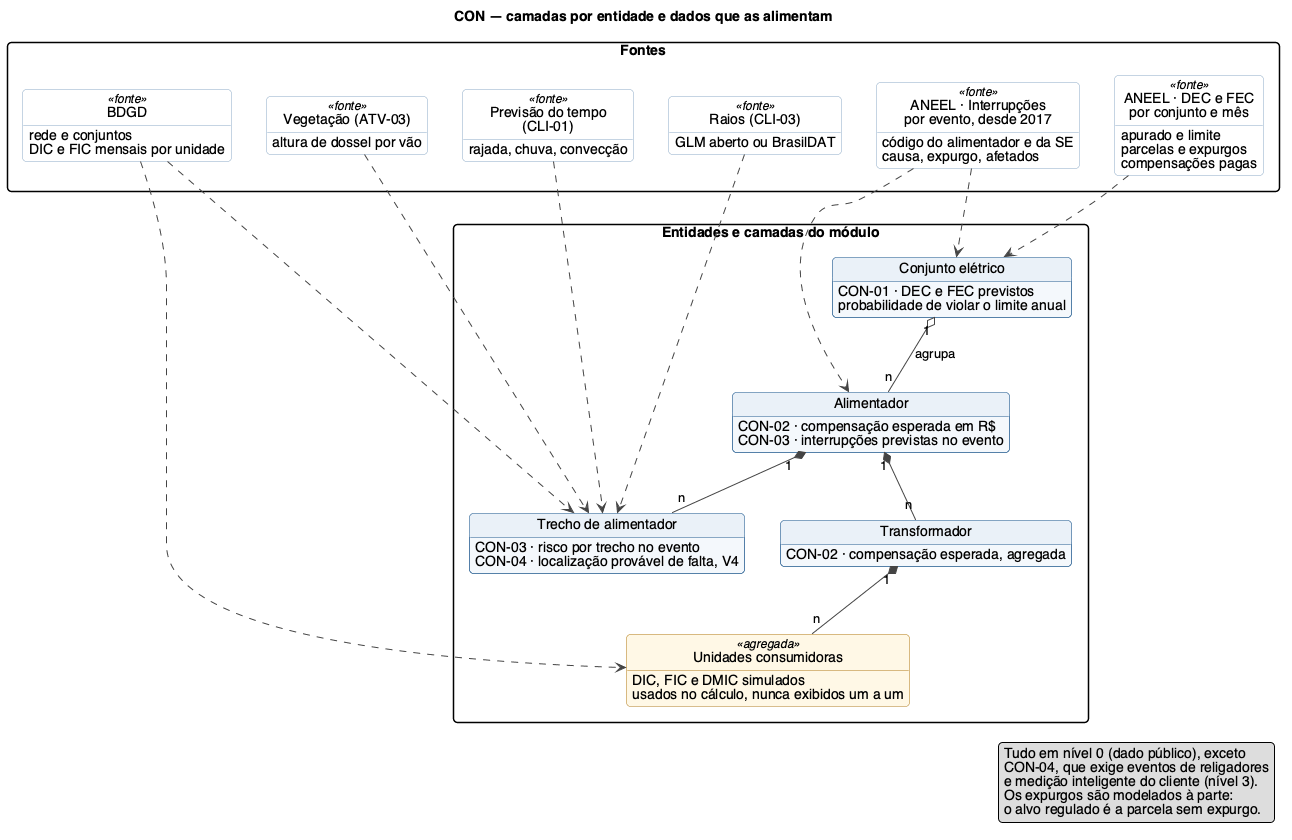
\includegraphics[width=\textwidth]{con-camadas.png}
\caption{CON: camadas por entidade e dados que as alimentam. Nível 0, exceto
CON-04; CON-02 exige nível 1 para o trimestre corrente.}
\end{figure}

\begin{figure}[H]
\centering
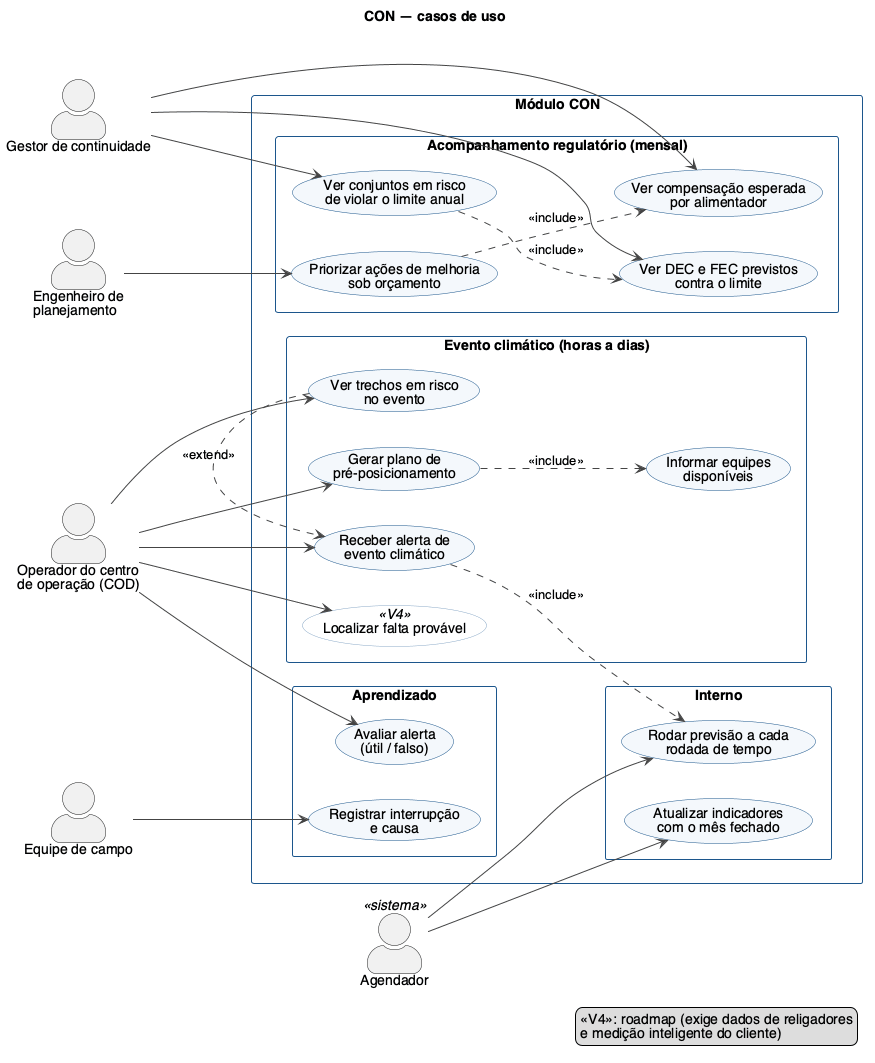
\includegraphics[width=0.78\textwidth]{con-casos-de-uso.png}
\caption{CON: casos de uso, separados pelos dois ritmos do módulo.}
\end{figure}

\begin{figure}[H]
\centering
\begin{minipage}[t]{0.40\textwidth}\centering
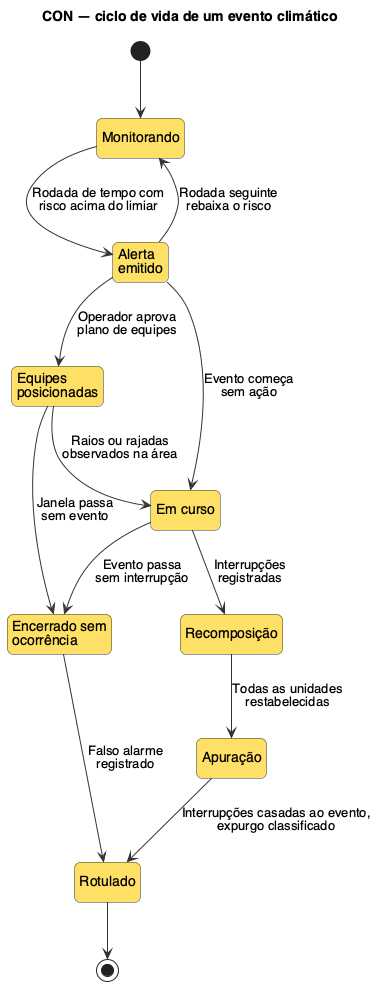
\includegraphics[width=\linewidth]{con-estados-evento.png}
\end{minipage}\hfill
\begin{minipage}[t]{0.56\textwidth}\centering
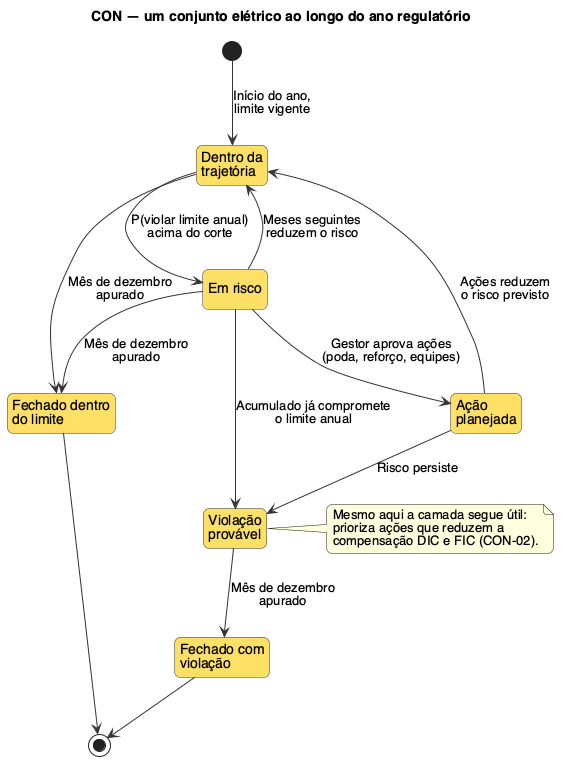
\includegraphics[width=\linewidth]{con-estados-conjunto.png}
\end{minipage}
\caption{CON: máquinas de estados do evento climático (esquerda) e do conjunto
elétrico no ano regulatório (direita). Eventos rotulados, inclusive falsos
alarmes, voltam como rótulos de treino.}
\end{figure}

\begin{figure}[H]
\centering
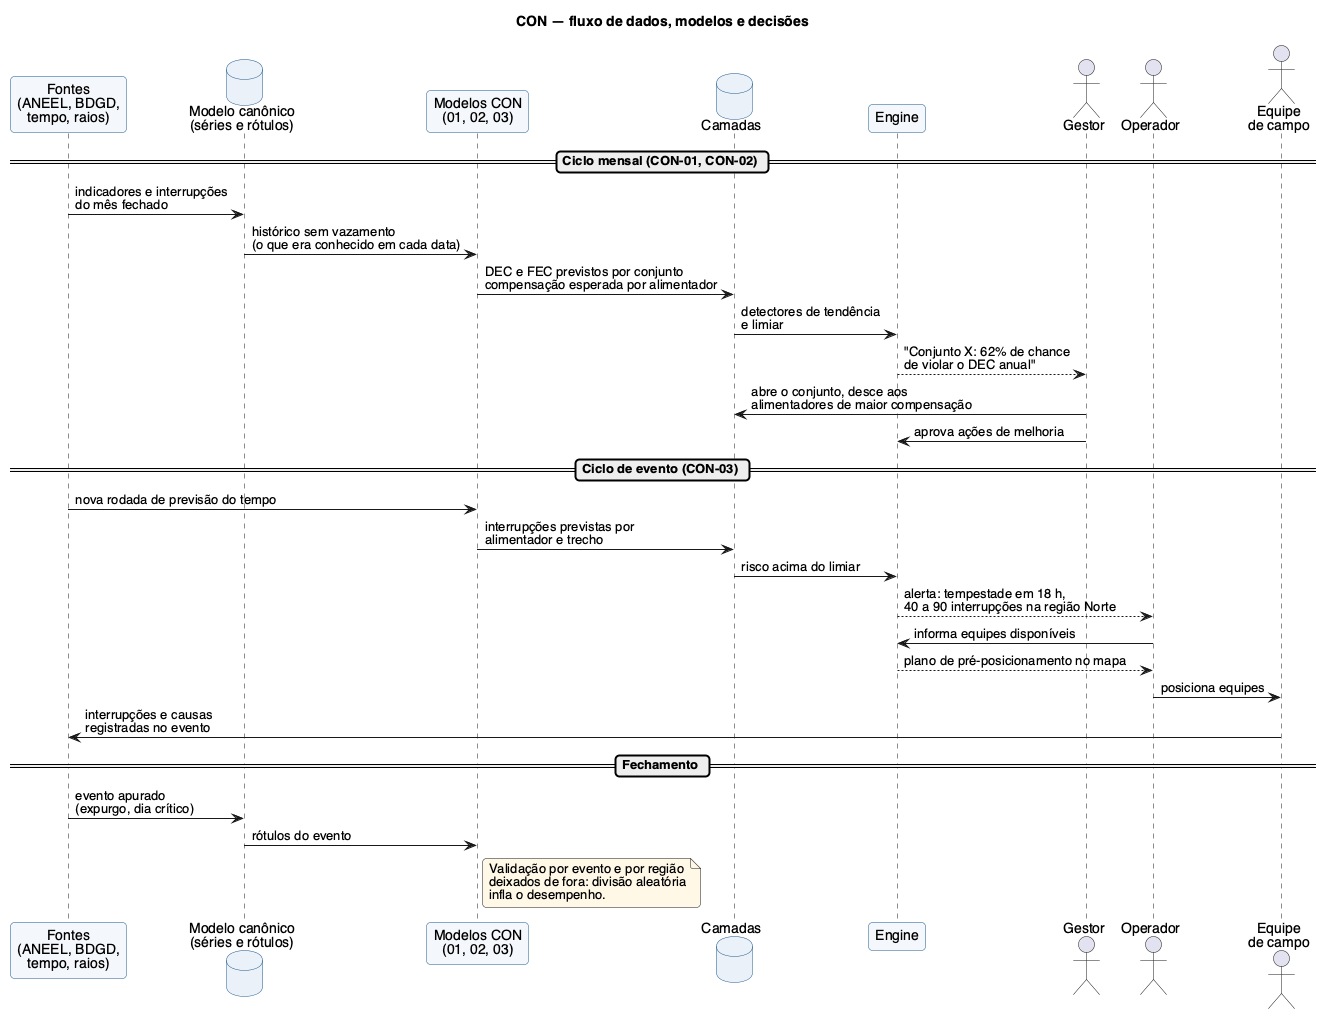
\includegraphics[width=\textwidth]{con-fluxo.png}
\caption{CON: fluxo do ciclo mensal, do ciclo de evento e do fechamento, com a
validação por evento e por região deixados de fora.}
\end{figure}

\subsection*{Referências desta seção}
{\small
\begin{enumerate}[label={[\arabic*]},leftmargin=2.2em,itemsep=1pt]
\item ANEEL, Indicadores Coletivos de Continuidade: \url{https://dadosabertos.aneel.gov.br/dataset/indicadores-coletivos-de-continuidade-dec-e-fec}
\item ANEEL, Interrupções nas Redes de Distribuição: \url{https://dadosabertos.aneel.gov.br/dataset/interrupcoes-de-energia-eletrica-nas-redes-de-distribuicao}
\item ANEEL, Ocorrências Emergenciais: \url{https://dadosabertos.aneel.gov.br/dataset/ocorrencias-emergenciais-nas-redes-de-distribuicao}
\item ANEEL, PRODIST Módulo 8 (REN 956/2021): \url{https://www.gov.br/aneel/pt-br/centrais-de-conteudos/procedimentos-regulatorios/prodist}
\item REN ANEEL 956/2021, PRODIST Módulo 1 (Dia Crítico)
\item ANEEL, BDGD: \url{https://dadosabertos.aneel.gov.br/dataset/base-de-dados-geografica-da-distribuidora-bdgd}
\item Radatz, bdgd2opendss: \url{https://github.com/PauloRadatz/bdgd2opendss}
\item Aderaldo (2023), BDGD-Tools, UFC: \url{https://repositorio.ufc.br/handle/riufc/75567}
\item[] \refstepcounter{enumi}
\item ONS, constrained-off por usina: \url{https://dados.ons.org.br/dataset/restricao_coff_eolica_detail}
\item ONS, RO-AO.BR.13, apuração de constrained-off
\item ONS Dados Abertos, linhas e disponibilidade: \url{https://dados.ons.org.br/dataset/linha-transmissao}
\item EPE, bases de dados de transmissão: \url{https://www.epe.gov.br/pt/leiloes-de-energia/leiloes-de-transmissao/bases-de-dados}
\item ANEEL, REN 729/2016 (Parcela Variável)
\item ANEEL, Plano de Desenvolvimento da Distribuição: \url{https://www.gov.br/aneel/pt-br/assuntos/distribuicao/plano-de-desenvolvimento-da-distribuicao}
\item INPE/ELAT, RINDAT e BrasilDAT: \url{http://www.inpe.br/webelat/rindat/}
\item NASA Earthdata, GLM: \url{https://www.earthdata.nasa.gov/data/instruments/glm}
\item INMET, BDMEP: \url{https://bdmep.inmet.gov.br/}
\item Wanik et al.\ (2015), \emph{Natural Hazards} 79, doi:10.1007/s11069-015-1908-2
\item Cerrai et al.\ (2019), \emph{IEEE Access} 7
\item UConn Outage Prediction Model, AGU (2021)
\item Extratropical storms outages, \emph{NHESS} 21 (2021)
\item Essus, Vatsavai e Rachunok (2026), vazamento em modelos de interrupção: \url{https://arxiv.org/abs/2608.24665}
\item Stanishevska e Guikema (2025): \url{https://arxiv.org/abs/2510.03959}
\item GNN e risco de árvores por LiDAR, \emph{RESS} (2025)
\item Lin et al.\ (2023), PowerFlowNet: \url{https://arxiv.org/abs/2311.03415}
\item Ghamizi et al.\ (2024), PowerFlowMultiNet: \url{https://arxiv.org/abs/2403.00892}
\item Okoyomon, Yaniv e Goebel (2025): \url{https://arxiv.org/abs/2509.25158}
\item PF$\Delta$ (2025): \url{https://arxiv.org/abs/2510.22048}
\item SafePowerGraph (2024): \url{https://arxiv.org/abs/2407.12421}
\item Nakiganda e Chatzivasileiadis, GNN para contingências: \url{https://arxiv.org/abs/2310.04213}
\item N-k com redes input-convex (2024): \url{https://arxiv.org/abs/2410.00796}
\item Baran e Wu (1989), \emph{IEEE Trans.\ Power Delivery} 4(2)
\item Jacob et al.\ (2024), \emph{Nature Communications}
\item PI-GNN para reconfiguração (2023): \url{https://arxiv.org/abs/2310.00728}
\item Karabulut, Manna e Develder (2026): \url{https://arxiv.org/abs/2604.20403}
\item Localização de faltas em BT com gêmeo digital, \emph{Energies} 16 (2023), doi:10.3390/en16237850
\item Alarme de sobrecarga em transformadores de distribuição (2024)
\item Investimento em redes de distribuição com correlação entre projetos, \emph{Frontiers in Energy Research} (2021)
\item Limites de interrupção no Brasil com IA, \emph{Energies} 16 (2023), doi:10.3390/en16197012
\item Predição de indicadores de qualidade com redes neurais, SBSE
\item IEEE C57.91, guia de carregamento
\end{enumerate}}

% Fichas de pesquisa: ATV, GER
% Conferido na web em 23/09/2026. "(a confirmar)" marca o que não foi verificado em fonte.

\section{Ativos e geração renovável}

\subsection*{Bases comuns}
\begin{itemize}
  \item \textbf{ONS Dados Abertos} (CC-BY, também espelhado no AWS) [8]: geração
    por usina em base horária [5], fator de capacidade horário de eólicas e
    solares [6], constrained-off semi-horário por usina desde 2021 [1--4],
    disponibilidade de linhas e transformadores [7]. O ONS avisa que os dados
    são revisados depois de publicados.
  \item \textbf{ANEEL}: SIGA (cadastro de usinas por CEG) [9], SIGEL (usinas e
    linhas em shapefile, aerogeradores no SIGEL-EOL) [10], BDGD [11],
    interrupções nas redes de distribuição [12].
  \item \textbf{Chave de junção}: o constrained-off traz \texttt{ceg} e
    \texttt{id\_ons} [4], o que liga ONS, SIGA e SIGEL pelo CEG; conjuntos de
    usinas aparecem sem CEG e exigem uma tabela de correspondência própria.
\end{itemize}

% ---------------------------------------------------------------------------
\subsection{ATV \textperiodcentered{} Ativos e manutenção}

\begin{ficha}{ATV-01 \textperiodcentered{} Índice de saúde de transformadores de potência}{V3}
\campo{Dados} Do cliente: cromatografia de gases dissolvidos (H$_2$, CH$_4$,
C$_2$H$_6$, C$_2$H$_4$, C$_2$H$_2$, CO, CO$_2$), físico-química do óleo,
furanos, carregamento, idade, histórico de ordens de serviço. Normas: IEC
60599:2022 [28]; IEEE C57.104-2019, que trocou limiares de gás total por
percentis por gás, deltas entre amostras e taxas anuais [27]; triângulos e
pentágonos de Duval [30]; índices de avaliação do CIGRE TB 761 [31]. Dados
públicos de referência: IEC TC10, com 117 amostras rotuladas [29].
\campo{Abordagens} Linha de base: regras normativas combinadas num índice
ponderado no estilo CIGRE. Recomendada: gradient boosting que usa as normas
como variáveis (razões, coordenadas de Duval, deltas, taxas, perda de vida
pelo IEEE C57.91 [33]), tendo como rótulo o evento posterior (falha ou
intervenção) e não a classe de Duval; com calibração e SHAP. Revisão recente:
Zahra et al.\ (2025) [32].
\campo{Métricas} F1 por classe de falha (diagnóstico); AUC-PR para falha ou
intervenção em 12 meses e acerto no topo da lista (prognóstico); concordância
com especialista.
\campo{Armadilhas} Validação só no IEC TC10 (117 amostras) não sustenta
generalização;
taxas exigem três ou mais amostras, raras na prática; troca de laboratório e
tratamento do óleo criam saltos artificiais.
\end{ficha}

\begin{ficha}{ATV-02 \textperiodcentered{} Risco de falha por equipamento}{V3}
\campo{Dados} Públicos: BDGD (segmentos, transformadores, chaves, data de
instalação) [11] e interrupções por evento [12]; ONS para a rede básica [7].
Do cliente: cadastro com trocas, ordens de serviço estruturadas (ATV-05).
\campo{Abordagens} Linha de base: Weibull por classe e Cox. Recomendada:
random survival forest ou boosting com perda de sobrevivência e covariáveis
que mudam no tempo (clima, carregamento), tratando censura e truncamento à
esquerda [34,35]. Literatura recente: DeepSurv e modelos neurais de tempo
discreto [36]. No nível do alimentador: contagem de falhas por km e ano.
\campo{Métricas} C-index (inclusive dependente do tempo), Integrated Brier
Score, calibração em 12 meses, acerto no topo da lista.
\campo{Armadilhas} Truncamento à esquerda (viés de sobrevivente); trocas sem
registro; causas externas misturadas com desgaste (riscos competitivos).
\end{ficha}

\begin{ficha}{ATV-03 \textperiodcentered{} Vegetação próxima à rede}{V3}
\campo{Dados} Geometria da rede (BDGD [11], SIGEL [10]). Altura de dossel
pública: mapa global de 10~m para 2020 (Lang et al.\ 2023) [37] e de 1~m
(Meta e WRI, Tolan et al.\ 2024, imagens de 2017 a 2020) [38]. Sentinel-2
para atualização. LiDAR do cliente quando houver.
\campo{Abordagens} Linha de base: altura de dossel e NDVI cruzados com um
buffer do vão. Recomendada: segmentação de vegetação densa e regressão de
altura com Sentinel-2 e GEDI; caso brasileiro (SENAI e Cemig, 2025/2026) com
RMSE de 7,7~m e MAE de 5~m contra LiDAR [39]. Com LiDAR: distância direta
entre condutor e vegetação. Literatura recente: SAM adaptado para corredores de
transmissão [40].
\campo{Métricas} IoU e F1 da segmentação; erro de altura contra LiDAR; recall
de vãos críticos em campo; correlação com interrupções por vegetação [12].
\campo{Armadilhas} Erro de 5 a 8~m é da ordem da faixa de segurança: serve
para priorizar, não para medir distância. Mapas estáticos envelhecem com
crescimento e poda.
\end{ficha}

\begin{ficha}{ATV-04 \textperiodcentered{} Defeitos em imagens de inspeção}{V4}
\campo{Dados} Imagens de drone do cliente. Públicos: CPLID (defeitos
sintéticos) [21]; InsPLAD, com 10.607 imagens, 17 classes de ativo e 6 tipos
de defeito, mas só 402 amostras de defeito [22]; TTPLA (torres e cabos) [23];
UPID [24].
\campo{Abordagens} Linha de base: YOLO ajustado para componentes [26].
Recomendada: dois estágios, detectar o componente e classificar o defeito ou
detectar anomalia no recorte [22]. Literatura recente: RT-DETR (CVPR 2024) [25];
SAM para pré-anotação com humano no ciclo.
\campo{Métricas} mAP por classe; recall por defeito crítico; precisão por
estrutura (o que vira ordem de serviço).
\campo{Armadilhas} Defeitos raros; modelos treinados em defeitos sintéticos
podem não generalizar; tipos de
isolador brasileiros diferem; cada imagem precisa ser associada à estrutura
da BDGD.
\end{ficha}

\begin{ficha}{ATV-05 \textperiodcentered{} Estruturação de ordens de serviço e causas}{V3}
\campo{Dados} Texto livre das ordens de serviço do cliente; causas do dataset
de interrupções como rótulo fraco [12]. Esquemas: MaintIE (224 entidades, 6
relações) [41] e ISO 14224 para modos de falha [42].
\campo{Abordagens} Na classificação de modo de falha em 22 códigos ISO 14224,
um GPT-3.5 ajustado chegou a F1 0,80, contra 0,60 de um classificador de
texto e 0,46 do modelo sem ajuste [42]. Recomendada: modelo de linguagem com
saída JSON restrita a um esquema (componente, modo de falha, causa, ação),
exemplos do cliente, ajuste leve e revisão humana por amostragem.
\campo{Métricas} F1 por campo; taxa de JSON válido; ganho de C-index em ATV-02
com as variáveis extraídas.
\campo{Armadilhas} Os benchmarks são em inglês e o texto das ordens é curto,
abreviado e regional; cada campo extraído precisa guardar o trecho que o
justifica; LGPD.
\end{ficha}

\begin{ficha}{ATV-06 \textperiodcentered{} Vida útil remanescente e plano de manutenção}{V4}
\campo{Dados} ATV-01 e ATV-02; custos, equipes e orçamento do cliente;
consequência da falha pelos clientes afetados (BDGD, interrupções).
\campo{Abordagens} Linha de base: matriz risco × criticidade. Recomendada:
risco monetizado por ativo e otimização inteira sob equipes e regiões (a
confirmar como padrão). Literatura recente: otimização estocástica sob a
incerteza da curva de sobrevivência.
\campo{Armadilhas} Poucos fins de vida para validar; a otimização amplifica
erros de calibração.
\end{ficha}

% ---------------------------------------------------------------------------
\subsection{GER \textperiodcentered{} Geração renovável}

\begin{ficha}{GER-01 \textperiodcentered{} Geração prevista por parque (P10--P90)}{V2}
\campo{Dados} Localização e ficha: SIGA e SIGEL [9,10]. \textbf{Geração
observada pública}: ONS por usina, horária [5], e geração verificada
semi-horária no constrained-off [4]; cobre usinas Tipo I, II-B e II-C (II-C
agregadas em conjuntos). Previsão do tempo: ECMWF abriu todo o catálogo em
tempo real sob CC-BY em outubro de 2025 [53]. SCADA do cliente em médias de
10 minutos.
\campo{Abordagens} Linha de base: persistência, climatologia, curva de
potência aplicada à previsão. Recomendada: gradient boosting quantílico sobre
variáveis da previsão numérica, o método vencedor do GEFCom2014 [52], com
recalibração conformal. Onboarding sem histórico: foundation models com a
previsão do tempo como covariável futura (Chronos-2 [46], TimesFM 2.5 [47],
Moirai 2.0 [48]); histórias sintéticas geradas por modelo físico reduziram o
erro de 1,7 a 2 vezes em 440 usinas fotovoltaicas [50]. Em [49], nenhuma
abordagem teve o menor erro em todos os casos. No Brasil, ERA5 superou o MERRA-2 para vento [54].
\campo{Métricas} nMAE e nRMSE pela capacidade; pinball e CRPS; cobertura
P10--P90; skill contra persistência; por horizonte e sem curtailment.
\campo{Armadilhas} \textbf{Treinar sobre a geração de referência, não sobre a
entregue}, para não aprender o curtailment [4]; revisões do ONS; vazamento
por tempo observado; UTC contra horário local.
\end{ficha}

\begin{ficha}{GER-02 \textperiodcentered{} Alertas de rampa}{V2}
\campo{Abordagens} Não há definição padrão: rampa é magnitude, duração
(tipicamente 1 a 4~h), instante e direção, com limiar pelo porte [55].
Linha de base: limiar de variação sobre a P50. Recomendada: probabilidade de
rampa calculada sobre \textbf{cenários coerentes no tempo}, não sobre quantis
marginais, que criam rampas espúrias.
\campo{Métricas} POD, FAR e CSI com tolerância de fase de uma hora; Brier;
antecedência; alertas por semana.
\end{ficha}

\begin{ficha}{GER-03 \textperiodcentered{} Nowcasting por satélite (0 a 6 h)}{V3}
\campo{Dados} GOES-19, GOES-East operacional desde 04/04/2025, no AWS sem
conta [13,14]; ABI com visível a 0,5~km e full disk a cada 10 minutos [15];
irradiância na superfície (DSR) a 2~km e 10 minutos no algoritmo Enterprise
[16]; radiação diária do INPE [17].
\campo{Abordagens} Linha de base: persistência do índice de céu claro e
vetores de movimento de nuvem. Recomendada: U-Net sobre sequências de índice
de nuvem, convertida em potência por usina [57,60]; caso brasileiro com
GOES-16 em Petrolina [59]. Literatura recente probabilístico: SHADECast, que
estende o horizonte útil em cerca de 26 minutos [56]. Acima de 2 a 3~h,
combinar com previsão numérica [53].
\campo{Métricas} RMSE de irradiância e potência; skill contra persistência
por antecedência; CRPS.
\campo{Armadilhas} Paralaxe e resolução contra usinas pequenas; latência;
descontinuidade na troca do GOES-16 para o GOES-19.
\end{ficha}

\begin{ficha}{GER-04 \textperiodcentered{} Curtailment detectado e marcado}{V2}
\campo{Dados} Constrained-off do ONS, dicionário v1.5 (09/2026): geração,
geração limitada, disponibilidade, referência, referência final (só para
REL, enviada à CCEE), razão (REL, CNF, ENE, PAR), origem (LOC, SIS), energia
não realizada e minutos por razão [4]. Relatório do GT Curtailment do ONS
[62]. SCADA com setpoints.
\campo{Abordagens} Linha de base: regras sobre a geração limitada e os
minutos de restrição; no SCADA, setpoint abaixo da nominal. Recomendada:
modelo de \textbf{potência disponível} (comportamento normal, GER-05);
curtailment é disponível menos entregue quando há limite, o que detecta
cortes não informados e contesta a referência do ONS; limpeza da curva de
potência por detecção de anomalias [64].
\campo{Armadilhas} Resolução de 30 minutos esconde cortes curtos; regras de
ressarcimento mudam por resolução (a confirmar).
\end{ficha}

\begin{ficha}{GER-05 \textperiodcentered{} Desempenho real × esperado}{V3}
\campo{Dados} SCADA, recurso, curtailment de GER-04. Públicos para
desenvolver: Kelmarsh e Penmanshiel (SCADA de 10 minutos, CC-BY) [18,19];
PVDAQ do NREL [68].
\campo{Abordagens} Linha de base: curva de potência por intervalos e
performance ratio. Recomendada: modelo de comportamento normal (boosting ou
GAM) treinado em período saudável; para fotovoltaica, pvlib ajustado.
Ferramentas: OpenOA (NREL) [65] e RdTools para degradação [71].
\campo{Armadilhas} Treinar o esperado sobre dados que já contêm a perda; a
limpeza pode reter só cerca de 31\% dos dados [64].
\end{ficha}

\begin{ficha}{GER-06 \textperiodcentered{} Saúde de turbinas}{V3}
\campo{Dados} SCADA com temperaturas de rolamentos, gerador e caixa
multiplicadora. Rotulados: CARE to Compare (Fraunhofer, 2024), 95 datasets, 36
turbinas, 44 eventos rotulados, com a métrica CARE (cobertura, acurácia,
confiabilidade, antecedência) [20].
\campo{Abordagens} Revisão: Tautz-Weinert e Watson (2017) [66]. Chesterman et
al.\ (2023), em 5 parques: Elastic Net competitivo com LightGBM e redes;
normalizar pela mediana da frota; excluir 4 meses antes da falha do treino;
nenhuma família domina [67]. Recomendada: comportamento normal com
normalização pela frota e alarme com persistência.
\campo{Métricas} CARE score; dias de antecedência; falsos alarmes por turbina
por ano.
\campo{Armadilhas} Poucas falhas; dados pré-falha contaminam o normal; clima
do Nordeste diferente do dos datasets europeus.
\end{ficha}

\begin{ficha}{GER-07 \textperiodcentered{} Sujidade e programação de limpeza solar}{V4}
\campo{Abordagens} Kimber (acúmulo linear até chuva acima de limiar) e HSU
(por massa de particulado), ambos no pvlib [69,70]; a partir da produção, SRR
(Deceglie et al.\ 2018) no RdTools [71]; relatório IEA PVPS T13-21:2022 [72].
Limiares de chuva que limpa variam de 0,3 a 20~mm/dia [73]. Decisão: limpar
quando a perda esperada até a próxima chuva prevista supera o custo.
\campo{Armadilhas} Confundir sujidade com degradação ou sombreamento;
limpezas não registradas quebram o SRR.
\end{ficha}

\begin{ficha}{GER-08 \textperiodcentered{} Geração agregada prevista por submercado}{cond}
\campo{Abordagens} Soma das previsões por usina com upscaling para as sem
previsão; reconciliação hierárquica (usina, estado, submercado) [74] e versão
orientada a valor [75]. Quantis agregados exigem cenários conjuntos: soma de
quantis não é o quantil da soma.
\campo{Armadilhas} Entrada de novas usinas (atualizar pelo SIGA); dizer se a
previsão é de potência disponível ou entregue; GD invisível.
\end{ficha}

\subsection*{Referências desta seção}
{\small
\begin{enumerate}[label={[\arabic*]},leftmargin=2.2em,itemsep=1pt]
\item ONS, constrained-off de eólicas: \url{https://dados.ons.org.br/dataset/restricao_coff_eolica_usi}
\item ONS, constrained-off de eólicas por usina: \url{https://dados.ons.org.br/dataset/restricao_coff_eolica_detail}
\item ONS, constrained-off de fotovoltaicas: \url{https://dados.ons.org.br/dataset/restricao_coff_fotovoltaica_detail}
\item ONS, dicionário do constrained-off v1.5 (09/2026)
\item ONS, geração por usina horária: \url{https://dados.ons.org.br/dataset/geracao-usina-2}
\item ONS, fator de capacidade: \url{https://dados.ons.org.br/dataset/fator-capacidade-2}
\item ONS, disponibilidade da função transmissão: \url{https://dados.ons.org.br/dataset/ind_disponibilidade_ft_trlt}
\item ONS no AWS: \url{https://registry.opendata.aws/ons-opendata-portal/}
\item ANEEL, SIGA: \url{https://dadosabertos.aneel.gov.br/dataset/siga-sistema-de-informacoes-de-geracao-da-aneel}
\item ANEEL, SIGEL: \url{https://sigel.aneel.gov.br/portal/home/}
\item ANEEL, BDGD: \url{https://dadosabertos.aneel.gov.br/dataset/base-de-dados-geografica-da-distribuidora-bdgd}
\item ANEEL, interrupções: \url{https://dadosabertos.aneel.gov.br/dataset/interrupcoes-de-energia-eletrica-nas-redes-de-distribuicao}
\item NOAA GOES no AWS: \url{https://registry.opendata.aws/noaa-goes/}
\item NOAA, GOES-19 no NODD
\item GOES-R ABI: \url{https://www.goes-r.gov/spacesegment/abi.html}
\item NCEI, ABI L2 DSR
\item INPE, radiação solar média diária (GOES-16)
\item Kelmarsh: \url{https://zenodo.org/records/5841834}
\item Penmanshiel: \url{https://zenodo.org/records/5946808}
\item Gück, Roelofs e Faulstich (2024), CARE to Compare: \url{https://arxiv.org/abs/2404.10320}
\item CPLID: \url{https://github.com/InsulatorData/InsulatorDataSet}
\item Vieira e Silva et al.\ (2023), InsPLAD, \emph{IJRS} 44(23): \url{https://arxiv.org/abs/2311.01619}
\item Abdelfattah et al.\ (2020), TTPLA: \url{https://arxiv.org/abs/2010.10032}
\item UPID: \url{https://github.com/heitorcfelix/public-insulator-datasets}
\item Zhao et al.\ (2024), RT-DETR, CVPR: \url{https://arxiv.org/abs/2304.08069}
\item MAP-YOLOv8, \emph{Scientific Reports} (2025)
\item IEEE C57.104-2019
\item IEC 60599:2022
\item IEC TC10 em \emph{IET GTD} (2021); IEEE DataPort DGA dataset
\item Duval, triângulos e pentágonos
\item CIGRE TB 761 (2019)
\item Zahra et al.\ (2025): \url{https://arxiv.org/abs/2504.15310}
\item IEEE C57.91, guia de carregamento
\item Modelos de sobrevivência em redes de energia, \emph{Sensors} (2026), doi:10.3390/s26061915
\item Ishwaran et al.\ (2008), Random Survival Forests, \emph{Ann.\ Appl.\ Stat.}
\item Katzman et al., DeepSurv: \url{https://arxiv.org/abs/1606.00931}
\item Lang et al.\ (2023), \emph{Nature Ecology \& Evolution} 7:1778--1789
\item Tolan et al.\ (2024), \emph{RSE} 300:113888: \url{https://registry.opendata.aws/dataforgood-fb-forests/}
\item HVAS (SENAI e Cemig), ISPRS Annals X-3-W4-2025
\item SAM para corredores de transmissão: \url{https://arxiv.org/abs/2505.22105}
\item Bikaun et al.\ (2024), MaintIE, LREC-COLING
\item Stewart et al., LLMs para modos de falha: \url{https://arxiv.org/abs/2309.08181}
\item Benchmark de LLMs em logs de turbinas: \url{https://arxiv.org/abs/2509.06813}
\item Extração de KPIs de ordens de serviço: \url{https://arxiv.org/abs/2311.04064}
\item Brundage et al., Technical Language Processing, \emph{Manufacturing Letters} 27
\item Ansari et al., Chronos-2: \url{https://arxiv.org/abs/2510.15821}
\item TimesFM 2.5: \url{https://huggingface.co/google/timesfm-2.5-200m-pytorch}
\item Moirai 2.0: \url{https://arxiv.org/abs/2511.11698}
\item Za'ter e Hodge (2026): \url{https://arxiv.org/abs/2604.22077}
\item Longarini et al.\ (2026), histórias sintéticas: \url{https://arxiv.org/abs/2606.07457}
\item Chronos, TimesFM e Moirai, versões originais
\item Hong et al.\ (2016), GEFCom2014, \emph{IJF}; Landry et al., GBM
\item ECMWF, catálogo em tempo real aberto (2025)
\item Gruber et al., reanálises no Brasil: \url{https://arxiv.org/abs/1904.13083}
\item Gallego-Castillo et al.\ (2015), rampas, \emph{RSER} 52
\item Carpentieri et al., SHADECast: \url{https://arxiv.org/abs/2312.11966}
\item Straub et al.\ (2024), \emph{Solar RRL}
\item SunCast: \url{https://arxiv.org/abs/2201.06173}
\item GHI e DNI com GOES-16 em Petrolina, \emph{Int.\ J.\ Energy Environ.\ Eng.}
\item Nowcasting por satélite com deep learning, \emph{Solar Energy} (2024)
\item Shi et al., ConvLSTM: \url{https://arxiv.org/abs/1506.04214}
\item ONS, RT DGL-ONS 0189-2025, GT Curtailment
\item Canal Solar, cortes em 2026 (fonte secundária)
\item Limpeza de curva de potência em SCADA, \emph{Renewable Energy} (2022)
\item NREL OpenOA: \url{https://github.com/NREL/OpenOA}
\item Tautz-Weinert e Watson (2017), \emph{IET RPG} 11, doi:10.1049/iet-rpg.2016.0248
\item Chesterman et al.\ (2023), \emph{Wind Energy Science} 8:893
\item NREL PVDAQ: \url{https://data.openei.org/submissions/4568}
\item Modelo de sujidade de Kimber no pvlib
\item Modelo de sujidade HSU
\item RdTools SRR; Deceglie et al.\ (2018), \emph{IEEE JPV} 8(2)
\item IEA PVPS T13-21:2022, perdas por sujidade
\item Limpeza por chuva, \emph{Solar RRL} (2024)
\item Hansen et al.\ (2023), reconciliação espacial de previsões eólicas, \emph{Wind Energy}
\item Reconciliação orientada a valor: \url{https://arxiv.org/abs/2501.16086}
\end{enumerate}}

% Fichas de pesquisa: MER, CLI, DRE, ENG
% Conferido na web em 23/09/2026. "(a confirmar)" marca o que não foi verificado em fonte.

\section{Mercado, clima, resposta da demanda e engine}

% ---------------------------------------------------------------------------
\subsection{MER \textperiodcentered{} Mercado e preço}

\begin{nota}
\textbf{Trilha condicional.} As três features deste módulo, com CAR-08 e
GER-08, estão fora do roadmap faseado: entram apenas se a questão de
cliente-alvo for resolvida a favor de gerador e comercializadora. A pesquisa
fica registrada para que a decisão, quando vier, não recomece do zero.
\end{nota}

\begin{nota}
\textbf{Acesso aos dados da CCEE.} O portal Dados Abertos da CCEE tem um bloqueio
de segurança (firewall de aplicação) que barra clientes fora da política de
acesso e orienta a abrir chamado com o código do erro e o IP [1,2]. A
CCEE divulga tutoriais de automação por API, e o download de um endpoint
CKAN (\texttt{/datastore/dump/<id>}) funcionou sem bloqueio em 23/09/2026. A
coleta automatizada foi possível com poucas requisições, user-agent
identificável, cache local e download dos CSVs anuais em vez de raspagem.
\end{nota}

\begin{ficha}{MER-01 \textperiodcentered{} PLD previsto por submercado (quantis)}{cond}
\campo{Dados} \emph{PLD\_HORARIO} da CCEE: um CSV por ano, horário de 2021 a
2026 e semanal de 2001 a 2020, licença CC-BY 4.0, atualização diária [3].
Limites regulatórios de 2026: piso R\$~57,31/MWh, teto estrutural
R\$~785,27/MWh e teto horário R\$~1.611,04/MWh (Despacho ANEEL 3.850/2025)
[5]. Decks NEWAVE/DECOMP/DESSEM no Acervo CCEE, inclusive decks sombra [6];
decks do DESSEM também no ONS [7]. ONS Dados Abertos: carga semi-horária,
geração por usina e CMO semi-horário [8].
\campo{Abordagens} Linha de base: ingênuo sazonal e LEAR (autorregressivo
com LASSO), usado como referência e implementado no \emph{epftoolbox} [10].
Recomendada: gradient boosting com perda quantílica sobre CMO, carga e
renováveis previstas, armazenamento dos reservatórios e deck vigente, com
calibração conformal (a confirmar). Literatura recente: emulação do DESSEM por
modelo substituto e redes que preveem distribuições paramétricas [10].
\campo{Métricas} Pinball e CRPS, cobertura e largura dos intervalos, MAE
relativo ao ingênuo, teste de Diebold--Mariano.
\campo{Armadilhas} Quebra estrutural em 01/01/2021 (PLD passou a horário,
calculado pelo DESSEM) [4]; nova função de custo futuro em 12/10/2025 [6];
distribuição censurada no piso e no teto; séries do ONS revisadas depois de
publicadas, o que exige guardar o que era conhecido em cada data [8]. O
Projeto Meta II propõe preço por oferta e dois PLDs (ex-ante e ex-post), com
implantação prevista para junho de 2028 [9], o que quebrará a série se implantado.
\end{ficha}

\begin{ficha}{MER-02 \textperiodcentered{} Cenários conjuntos de geração, carga e preço}{cond}
\campo{Dados} Saídas probabilísticas de GER-01, CAR-08 e MER-01; histórico
conjunto do ONS e da CCEE [3,8].
\campo{Abordagens} Linha de base: cenários independentes ou bootstrap de
blocos históricos. Recomendada: cópula gaussiana sobre as marginais
preditivas (Pinson et al.\ 2009) [11]; alternativa com a ordem dos membros do
ensemble meteorológico (ECC e dual-ECC) [12]. Literatura recente: cópulas vine e
geradores profundos (a confirmar).
\campo{Métricas} Energy score e variogram score, histogramas de posto
multivariados, CRPS por marginal (biblioteca \emph{scoringrules}) [13].
\campo{Armadilhas} A dependência muda com o regime hidrológico, e uma cópula
estacionária subestima eventos conjuntos extremos (seca com pico de carga).
\end{ficha}

\begin{ficha}{MER-03 \textperiodcentered{} Otimização de oferta e despacho de baterias}{cond}
\campo{Dados} Cenários de MER-02, PLD horário e parâmetros técnicos da
bateria. Contexto: Portaria MME 136/2026 define o primeiro leilão de reserva
de capacidade em baterias (dezembro de 2026, contratos de 15 anos a partir
de agosto de 2028), com receita de disponibilidade e não de arbitragem livre
[14].
\campo{Abordagens} Linha de base: otimização determinística sobre a previsão
pontual. Recomendada: programação estocástica em dois estágios ou CVaR,
em janela móvel. Literatura recente: aprendizado focado na decisão; minimizar o
CRPS não garante a melhor oferta [15].
\campo{Métricas} Receita contra o ótimo com informação perfeita (regret),
CVaR da receita, custo de degradação.
\campo{Armadilhas} Hoje o PLD vem de modelo de custo, não de ofertas; ``oferta''
só faz sentido com o modelo híbrido (2028 em diante) [9]. Degradação
simplificada superestima receita. Baixo encaixe com o mapa.
\end{ficha}

% ---------------------------------------------------------------------------
\subsection{CLI \textperiodcentered{} Contexto climático}

\begin{ficha}{CLI-01 \textperiodcentered{} Tempo previsto}{V2}
\campo{Dados} ECMWF Open Data: IFS e AIFS (determinístico e ensemble), grade
de 0,25°, quatro rodadas por dia, licença CC-BY 4.0 com uso comercial
permitido e atribuição obrigatória; o portal guarda só as rodadas dos
últimos 2 a 3 dias, com espelhos em nuvem [16,17]. NOAA GFS 0,25° no AWS,
aberto, com histórico longo no NCAR [18]. CPTEC/INPE: BAM, WRF, Eta e BRAMS,
com citação exigida [19]. INMET: estações automáticas horárias (portal com
90 dias) e BDMEP para o histórico, com defasagem de 1 a 3 meses [20].
\campo{Abordagens} Linha de base: previsão bruta interpolada para as
entidades. Recomendada: pós-processamento estatístico por entidade (MOS,
EMOS, regressão quantílica) com downscaling. Literatura recente: modelos globais
de ML (AIFS, GraphCast-GFS) [16,18]. Ferramentas: \emph{herbie},
\emph{xarray}/\emph{cfgrib}, \emph{xskillscore} [17].
\campo{Métricas} RMSE e MAE por variável e horizonte, CRPS do ensemble,
diagrama de confiabilidade, skill contra climatologia e persistência.
\campo{Armadilhas} \textbf{Arquivar cada rodada desde o primeiro dia}: sem
isso, não há histórico de previsões para treinar sem vazamento. Mudanças de
versão dos modelos quebram o pós-processamento. A atribuição do ECMWF precisa
aparecer no mapa.
\end{ficha}

\begin{ficha}{CLI-02 \textperiodcentered{} Satélite e radar observados}{V2}
\campo{Dados} GOES-East é o \textbf{GOES-19} desde abril de 2025 (75,2°W),
com ABI e GLM no AWS Open Data em NetCDF4; houve interrupções (ABI restaurado
em julho de 2026) [21]. Radar REDEMET/DECEA por API com chave, mas em imagem
PNG, útil para exibir e não para modelar [22]. CEMADEN: pluviômetros e radares
de dupla polarização, com dados volumétricos sob solicitação (a confirmar)
[23].
\campo{Abordagens} Linha de base: exibir mosaicos. Recomendada: nowcasting de
precipitação de 0 a 6 h com \emph{pysteps} (fluxo óptico e ensembles
estocásticos) [24]. Literatura recente: nowcasting profundo (ConvGRU, difusão).
\campo{Métricas} CSI, POD e FAR por limiar; FSS; CRPS [24].
\campo{Armadilhas} Cobertura de radar desigual no território; lacunas e
latência do GOES.
\end{ficha}

\begin{ficha}{CLI-03 \textperiodcentered{} Raios e eventos severos}{V3}
\campo{Dados} BrasilDAT (ELAT/INPE): detecta descargas nuvem-solo e
intranuvem; acesso por contato com o ELAT, \textbf{não é aberta} [25].
Alternativa aberta: GLM do GOES-19, detecção óptica de raios totais com
eficiência uniforme sobre o Brasil [21,26].
\campo{Abordagens} Densidade de descargas por célula e janela; cruzamento
espaço-temporal de raios com desligamentos de alimentadores (alimenta
CON-03).
\campo{Métricas} POD e FAR dos alertas contra desligamentos; antecedência.
\campo{Armadilhas} O GLM registra flashes ópticos, não pontos de impacto, com
localização da ordem de quilômetros (a confirmar): não serve para associar
descarga a vão de linha.
\end{ficha}

% ---------------------------------------------------------------------------
\subsection{DRE \textperiodcentered{} Resposta da demanda e consumidor}

\begin{ficha}{DRE-01 \textperiodcentered{} Alvos de resposta da demanda por alimentador}{V4}
\campo{Dados} Regulação: REN ANEEL 1.040/2022 (programa estrutural) e sandbox
do ONS para o produto disponibilidade, com primeiro mecanismo competitivo em
outubro de 2024 (até 4 acionamentos mensais de 4 h, entre 18 h e 22 h)
[27,28]. Resultados na CCEE [28]. O programa do ONS mira grandes consumidores
do SIN; resposta da demanda por alimentador é caso da distribuidora e depende
de medição própria (a confirmar).
\campo{Abordagens} Linha de base de medição: regras ``X de Y dias'' (a
confirmar). Recomendada: baseline contrafactual por ML, avaliada como
contrafactual porque define pagamento; literatura recente: controle sintético
generalizado e baselines probabilísticos [29]. Alvos: alimentadores com
carregamento previsto acima do limite (CAR-01, RED-01), ordenados por alívio
esperado por custo.
\campo{Métricas} Viés da baseline em dias sem evento; precisão no topo dos
alimentadores escolhidos; MW reduzidos contra contratados.
\campo{Armadilhas} Baseline enviesada paga indevidamente ou incentiva inflar
a carga antes do evento; efeito rebote; poucos eventos para validar.
\end{ficha}

\begin{ficha}{DRE-02 \textperiodcentered{} Desagregação de consumo (NILM)}{fora}
\campo{Dados} Medição agregada de alta frequência por unidade; bases públicas
REDD e UK-DALE; nenhuma base brasileira encontrada [30].
\campo{Abordagens} FHMM (NILMTK) como linha de base; seq2point (Zhang et
al.\ 2018) como recomendada [30].
\campo{Por que fica fora} Exige dado individual de alta frequência que não
existe em escala, o parque de aparelhos brasileiro (chuveiro elétrico) difere
das bases de treino, e a saída é por unidade consumidora, não espacial.
\end{ficha}

\begin{ficha}{DRE-03 \textperiodcentered{} Recomendação tarifária e de eficiência}{fora}
\campo{Dados} Tarifa Branca desde 2018, adesão de cerca de 69 mil unidades em
75 milhões aptas [31,32]; proposta da área técnica da ANEEL (novembro de 2025)
de Tarifa Branca automática para consumo acima de 1 MWh/mês, levada a consulta
pública, desfecho não verificado [32]. Tarifas homologadas por distribuidora
nos dados abertos da ANEEL [33].
\campo{Por que fica fora} Sem curva horária medida a recomendação é
especulativa, e a decisão é da unidade consumidora, não de uma entidade do
mapa. Se a Tarifa Branca automática for aprovada, a versão agregada (quantas
unidades de um alimentador seriam afetadas) pode voltar como insight.
\end{ficha}

% ---------------------------------------------------------------------------
\subsection{ENG \textperiodcentered{} Engine de análise e modelos}

\begin{ficha}{ENG-01 \textperiodcentered{} Feed de insights consolidado}{MVP}
\campo{Dados} Todas as camadas com a hierarquia, uma matriz de vizinhança
(geográfica ou por topologia elétrica) e o histórico por ciclo.
\campo{Abordagens} \emph{Pontuação}: adotar o esquema de Top-K Insights
(SIGMOD 2017) e QuickInsights (SIGMOD 2019, base do recurso do Power BI):
tipo de insight, subespaço e pontuação por impacto × significância [34].
\emph{Anomalia espacial}: Moran local (LISA) e Getis--Ord $G_i^*$ em
PySAL/\emph{esda}, com pseudo-p por permutação [35], sempre com controle de
FDR para testes múltiplos e dependentes [36]. \emph{Mudança e tendência}:
pontos de mudança offline com \emph{ruptures} e online com BOCPD [37];
excedência de quantil da previsão para limiares. \emph{Consolidação}: o
insight do pai absorve os dos filhos quando explica a maior parte do efeito;
a reconciliação MinT garante números coerentes entre níveis [38].
\campo{Métricas} Precisão no topo do feed (insights marcados úteis ou
acionados), taxa de falsos positivos sob dados embaralhados, insights por
evento real.
\campo{Armadilhas} Explosão de testes (entidades × camadas × detectores);
MAUP (o resultado muda com a escala de agregação); vizinhança geográfica não
é conectividade elétrica; fadiga de alertas.
\end{ficha}

\begin{ficha}{ENG-02 \textperiodcentered{} Explicação por entidade}{MVP}
\campo{Abordagens} TreeSHAP para modelos de árvore [39]; TimeSHAP para
modelos de séries [40]; GeoShapley para modelos espaciais, que trata a
localização como um jogador conjunto [41].
\campo{Métricas} Fidelidade (remoção e inserção), estabilidade entre
execuções, consistência com a física (sinal esperado da temperatura sobre a
carga).
\campo{Armadilhas} Variáveis climáticas correlacionadas dão atribuições
diferentes conforme a variante de SHAP [39]; explicação não é causa e não
deve alimentar a simulação de cenário como se fosse efeito.
\end{ficha}

\begin{ficha}{ENG-03 \textperiodcentered{} Erro dos modelos por entidade}{MVP}
\campo{Dados} Pares previsto × realizado, versionados por data de emissão,
horizonte e versão do modelo; realizados revisados pelo ONS e pela CCEE
exigem guardar a versão conhecida em cada data [8].
\campo{Métricas} nMAE com normalização explícita; CRPS (regra estritamente
própria) [42]; pinball; calibração (PIT, cobertura, confiabilidade) e
nitidez; precisão no topo para rankings. Bibliotecas: \emph{scoringrules}
(ativa, univariada e multivariada) e \emph{xskillscore}; a
\emph{properscoring} está pouco mantida [42].
\campo{Armadilhas} nMAE explode em entidades de carga baixa; métricas
agregadas escondem a cauda; poucas amostras por entidade pedem intervalo por
bootstrap antes de emitir o insight de desempenho.
\end{ficha}

\begin{ficha}{ENG-04 \textperiodcentered{} Deriva de dados por região}{V2}
\campo{Abordagens} Testes univariados (KS, PSI, Wasserstein) como no
\emph{Evidently} [43]; MMD para deriva multivariada; estimativa de desempenho
sem rótulo com NannyML [45]; testes de duas amostras sobre representações
reduzidas funcionam melhor segundo Rabanser et al.\ (2019) [46]. Aplicar o
teste por região e procurar agrupamentos de deriva com LISA (proposta, a
confirmar como prática).
\campo{Armadilhas} \textbf{Licença}: o \emph{alibi-detect} mudou de Apache 2.0
para Business Source License 1.1 em janeiro de 2024, com restrição a uso
comercial em produção [44]. Com amostras grandes, diferenças pequenas ficam estatisticamente
significativas: usar
tamanho de efeito e FDR; comparar com a mesma estação do ano.
\end{ficha}

\begin{ficha}{ENG-05 \textperiodcentered{} Simulação de cenário}{V2}
\campo{Abordagens} Perturbar entradas e reexecutar os modelos, alterando de
forma coerente variáveis correlacionadas e sinalizando extrapolação fora do
domínio de treino. Onde houver cenários conjuntos (MER-02, na trilha
condicional), propagar a incerteza sobre eles; sem eles, perturbar as
marginais e declarar que a dependência não está modelada.
Literatura recente: modelos causais estruturais (a confirmar: DoWhy, EconML).
\campo{Métricas} Backtest em choques históricos conhecidos; cobertura dos
intervalos.
\campo{Armadilhas} Modelos preditivos não são causais; o usuário pode ler o
cenário como previsão.
\end{ficha}

\begin{ficha}{ENG-06 \textperiodcentered{} Pergunta em texto livre}{V2}
\campo{Estado da técnica} Em text-to-SQL sobre bancos reais (BIRD), o melhor
sistema reportado em 2025 chega a cerca de 82\% de acurácia de execução contra 93\% de humanos
[47]. Em tarefas geoespaciais, agentes frequentemente ``alucinam'' relações
espaciais em vez de computá-las [48]. No DataGemma, mesmo com recuperação de
dados, parte relevante das estatísticas citadas saiu errada [49]: o modelo de
linguagem não pode ser fonte de número.
\campo{Arquitetura recomendada} (1) o modelo escolhe ferramentas de uma API
semântica restrita (métricas, entidades, filtros); SQL livre só como recurso
de exceção, em leitura e com limites; (2) a engine executa e devolve números
com identificadores; (3) o texto é redigido com marcadores preenchidos pela
engine; (4) um verificador rejeita a resposta se algum número não vier do
resultado; (5) a resposta cita os insights e consultas e admite ``não sei''.
\campo{Métricas} Acurácia de execução num conjunto próprio de perguntas do
setor; taxa de números sem fonte (meta: zero); taxa de recusa correta.
\campo{Armadilhas} Unidade errada (MW e MWh); nomes de subestação repetidos;
injeção de instruções vinda de texto nos dados; acesso a dados de unidades
consumidoras (controle por papel na camada de ferramentas).
\end{ficha}

\subsection*{Referências desta seção}
{\small
\begin{enumerate}[label={[\arabic*]},leftmargin=2.2em,itemsep=1pt]
\item CCEE Dados Abertos, mensagem de bloqueio: \url{https://dadosabertos.ccee.org.br/}
\item CCEE Dados Abertos, sobre e contatos: \url{https://dadosabertos.ccee.org.br/about}
\item CCEE, PLD\_HORARIO: \url{https://dadosabertos.ccee.org.br/dataset/pld_horario}
\item CCEE, conceitos de preços: \url{https://www.ccee.org.br/precos/conceitos-precos}
\item ANEEL, PLD 2026: \url{https://www.gov.br/aneel/pt-br/assuntos/noticias/2025/aneel-define-tarifas-de-energia-de-otimizacao-de-servicos-ancilares-e-pld-para-2026}
\item CCEE, Acervo e novas funções de custo futuro: \url{https://www.ccee.org.br/acervo-ccee}
\item ONS, decks do DESSEM: \url{https://www.ons.org.br/}
\item ONS Dados Abertos: \url{https://dados.ons.org.br/}
\item CCEE, Projeto Meta II: \url{https://www.ccee.org.br/en/web/guest/-/ccee-apresenta-primeiros-resultados-do-projeto-meta-ii-sobre-formacao-de-preco-no-brasil}
\item Lago et al.\ (2021), \emph{Applied Energy} 293:116983; \url{https://github.com/jeslago/epftoolbox}
\item Pinson et al.\ (2009), \emph{Wind Energy} 12:51--62, doi:10.1002/we.284
\item Ben Bouallègue et al.\ (2016), dual-ECC, \emph{Monthly Weather Review} 144(12)
\item scoringrules: \url{https://scoringrules.readthedocs.io/}
\item MME, diretrizes do leilão de baterias: \url{https://www.gov.br/mme/}
\item Decision-focused predict-then-bid: \url{https://arxiv.org/abs/2505.01551}; CRPS e decisão: \url{https://arxiv.org/abs/2308.15443}
\item ECMWF Open Data: \url{https://www.ecmwf.int/en/forecasts/datasets/open-data}
\item Herbie: \url{https://herbie.readthedocs.io/}
\item GFS no AWS: \url{https://registry.opendata.aws/noaa-gfs-pds/}; NCAR d084001
\item CPTEC/INPE: \url{https://previsaonumerica.cptec.inpe.br/}
\item INMET BDMEP: \url{https://bdmep.inmet.gov.br/}
\item GOES no AWS: \url{https://registry.opendata.aws/noaa-goes/}; NCEI ABI/GLM
\item API REDEMET, radar: \url{https://ajuda.decea.mil.br/base-de-conhecimento/api-redemet-produtos-radar/}
\item CEMADEN, mapa interativo: \url{https://mapainterativo.cemaden.gov.br/}
\item Pulkkinen et al.\ (2019), pysteps, \emph{GMD} 12:4185
\item ELAT/INPE, BrasilDAT: \url{https://www.gov.br/inpe/}
\item GLM, eficiência de detecção: \url{https://ntrs.nasa.gov/citations/20180000609}
\item REN ANEEL 1.040/2022: \url{https://www2.aneel.gov.br/cedoc/ren20221040.html}
\item CCEE e ONS, sandbox de resposta da demanda: \url{https://www.ccee.org.br/resposta-demanda}
\item Controle sintético para baseline de RD: \url{https://arxiv.org/abs/2604.18469}
\item Zhang et al.\ (2018), seq2point, AAAI-18; \url{https://github.com/nilmtk/nilmtk-contrib}
\item ANEEL, Tarifa Branca: \url{https://www.gov.br/aneel/pt-br/assuntos/tarifas/tarifa-branca}
\item Agência iNFRA, Tarifa Branca automática (2025)
\item ANEEL, tarifas homologadas: \url{https://dadosabertos.aneel.gov.br/dataset/tarifas-distribuidoras-energia-eletrica}
\item Tang et al.\ (2017), Top-K Insights, SIGMOD; Ding et al.\ (2019), QuickInsights, SIGMOD, doi:10.1145/3299869.3314037
\item PySAL esda: \url{https://pysal.org/esda/}
\item Caldas de Castro e Singer (2006), FDR em LISA, \emph{Geographical Analysis}
\item Truong et al.\ (2020), ruptures, \emph{Signal Processing}; Adams e MacKay (2007), BOCPD
\item Wickramasuriya, Athanasopoulos e Hyndman (2019), MinT, \emph{JASA} 114(526)
\item Lundberg et al.\ (2020), TreeSHAP, \emph{Nature Machine Intelligence} 2:56--67
\item Bento et al.\ (2021), TimeSHAP, KDD
\item Li (2024), GeoShapley, \emph{Annals of the AAG} 114(7)
\item Gneiting e Raftery (2007), \emph{JASA}; properscoring; xskillscore
\item Evidently: \url{https://github.com/evidentlyai/evidently}
\item alibi-detect, licença: \url{https://github.com/SeldonIO/alibi-detect/blob/master/LICENSE}
\item NannyML: \url{https://nannyml.readthedocs.io/}
\item Rabanser, Günnemann e Lipton (2019), Failing Loudly, NeurIPS
\item BIRD e Agentar-Scale-SQL: \url{https://arxiv.org/abs/2509.24403}
\item GeoBenchX: \url{https://arxiv.org/abs/2503.18129}
\item DataGemma: \url{https://arxiv.org/abs/2409.13741}
\end{enumerate}}


\end{document}
